\documentclass[12pt]{extarticle} % Utilizza il pacchetto extsizes per impostare la dimensione del font a 14pt
\usepackage{graphicx} % Required for inserting images
\usepackage[utf8]{inputenc}
\usepackage{amsmath}
\usepackage{titlesec}
\usepackage{titling}
\usepackage{xcolor}
\usepackage{txfonts}
\usepackage{amsfonts}
\usepackage[shortlabels]{enumitem}
\usepackage{latexsym}
\usepackage{fixmath}
\usepackage{hyperref}
\usepackage{amssymb}
\usepackage[italian]{babel}
\usepackage{gensymb}
\usepackage{centernot}
\usepackage{tikz}
\usetikzlibrary{automata, positioning, arrows.meta}
\usepackage{mdframed}
\usepackage{listings}
\usepackage[T1]{fontenc}
\usepackage[most]{tcolorbox}
\usepackage{lipsum}
\usepackage[top=2cm, bottom=2cm, left=2cm, right=2cm]{geometry}
\renewcommand{\iint}{\DOTSI\MultiIntegral{2}} % Redefine \iint to avoid conflict
\newcommand\independent{\protect\mathpalette{\protect\independenT}{\perp}}
\def\independenT#1#2{\mathrel{\rlap{$#1#2$}\mkern2mu{#1#2}}}

% Definizione del box azzurro per Esercizi ed Esempi
\newtcolorbox{eserciziobox}[1]{
    colback=blue!5!white,    % Sfondo azzurro molto chiaro
    colframe=blue!40!black,  % Bordo blu scuro
    fonttitle=\bfseries,
    title=#1,
    arc=2mm,                 % Angoli arrotondati
    boxrule=0.5mm,
    left=10pt,
    right=10pt,
    top=10pt,
    bottom=10pt,
    before skip=15pt,
    after skip=15pt,
    breakable                % Permette di spezzare il box su più pagine
}

\title{Calcolo delle Probabilità e Statistica}
\author{Matilde e Mattia\\CdL in Informatica}
\date{}

\definecolor{codegreen}{rgb}{0,0.5,0}

\begin{document}

% Define custom colors
\definecolor{codegreen}{rgb}{0,0.5,0}
\definecolor{codegray}{rgb}{0.5,0.5,0.5}   
\definecolor{codepurple}{rgb}{0.58,0,0.82}   
\definecolor{bluegreen}{rgb}{0,0.6,0.6}      
\definecolor{darkorange}{rgb}{1.0, 0.55, 0.0}
\definecolor{lightgray}{rgb}{0.83, 0.83, 0.83}
\definecolor{seashell}{rgb}{1.0, 0.96, 0.93}
\definecolor{lightyellow}{rgb}{1.0, 1.0, 1.0}
\definecolor{ghostwhite}{rgb}{0.97, 0.97, 1.0}
\definecolor{deepcarrotorange}{rgb}{0.91, 0.41, 0.17}
\definecolor{aqua}{rgb}{0.0, 1.0, 1.0}
\definecolor{aquamarine}{rgb}{0.5, 1.0, 0.83}
\definecolor{blue-violet}{rgb}{0.54, 0.17, 0.89}
\definecolor{beaver}{rgb}{0.62, 0.51, 0.44}

\lstdefinestyle{mystyle}{
    backgroundcolor=\color{ghostwhite},   
    identifierstyle=\color{black},
    commentstyle=\color{codegreen},
    keywordstyle=\color{blue-violet}\bfseries,
    numberstyle=\tiny\color{bluegreen},     
    stringstyle=\color{blue},    
    basicstyle=\ttfamily\small, % Keep code black but monospaced
    breakatwhitespace=false,   
    breaklines=true,              
    captionpos=b,              
    keepspaces=true,             
    numbers=left,               
    numbersep=5pt,              
    showspaces=false,           
    showstringspaces=false,      
    showtabs=false,             
    tabsize=2,
    morekeywords={exp, logspace, print, Exception, try, catch, from, import, while, True, False, },
    emphstyle=\color{blue}\bfseries, % Types in blue
    emph={[2]null}, % Highlight "null"
    emphstyle={[2]\color{deepcarrotorange}\bfseries}, % Apply deepcarrotorange
    emph={[3]size, length},
    emphstyle={[3]\color{deepcarrotorange}\bfseries},
    morestring=[b]", % Strings in blue
    morestring=[b]', % Single-character strings in blue
}



\lstset{style=mystyle}

\maketitle

\newpage

\tableofcontents
\newpage

\section{Spazi di probabilità}
\begin{itemize}
    \item $ \mathbb{P}(A) \approx \frac{\text{n. di volte che si verifica } A \text{ nel campione}}{n} $
    
    \item \textbf{Operazioni insiemistiche}:
        \begin{itemize}
            \item $A \cup B = \{\omega \in \Omega : \omega \text{ appartiene ad almeno uno tra } A \text{ e } B\}$
            \item $A_1 \cup A_2 \cup \dots \cup A_n = \{\omega \in \Omega : \omega \text{ appartiene ad almeno un insieme tra } A_1, A_2, \dots, A_n\}$
            \item $A \cap B = \{\omega \in \Omega : \omega \text{ appartiene sia ad } A \text{ che a } B\}$
            \item $A_1 \cap A_2 \cap \dots \cap A_n = \{\omega \in \Omega : \omega \text{ appartiene a tutti gli insiemi } A_1, A_2, \dots, A_n\}$
            \item $A^c = \{\omega \in \Omega : \omega \text{ non appartiene ad } A\}$
            \item $ B \setminus A = \{\omega \in B : \omega \text{ non appartiene ad } A\}. $
        \end{itemize}

    \vspace{0.3cm}
    
    \item $ (A \cup B)^c = A^c \cap B^c $
    \item $ (A \cap B)^c = A^c \cup B^c $

    \item $ A \cup (B \cap C) = (A \cup B) \cap (A \cup C) $
    \item $ A \cap (B \cup C) = (A \cap B) \cup (A \cap C) $

    \item $ \bigcup_{n=1}^{\infty} A_n = \{\omega \in \Omega : \omega \in A_n \text{ per almeno un } n\} $
    \item $ \bigcap_{n=1}^{\infty} A_n = \{\omega \in \Omega : \omega \in A_n \text{ per ogni } n\} $

    \item \textbf{De Morgan generalizzate} (valgono anche per famiglie infinite):
    $$ \Big(\bigcup_{n} A_n\Big)^c = \bigcap_n A_n^c, \qquad \Big(\bigcap_n A_n\Big)^c = \bigcup_n A_n^c $$

    \item \textbf{Distributive generalizzate}:
    $ A \cup \big(\bigcap_{i=1}^n B_i\big) = \bigcap_{i=1}^n (A \cup B_i), \quad A \cap \big(\bigcup_{i=1}^n B_i\big) = \bigcup_{i=1}^n (A \cap B_i) $

    \item \textbf{Insieme delle parti}: $\mathcal{P}(\Omega)$ = insieme di tutti i sottoinsiemi di $\Omega$ ($\emptyset$ e $\Omega$ compresi). Se $|\Omega| = n$ allora $ |\mathcal{P}(\Omega)| = 2^n $.
\end{itemize}

\paragraph{Traduzioni ricorrenti} (con $A, B, C$ eventi):
\begin{itemize}
    \item \textbf{almeno un evento si verifica}: $A \cup B \cup C$
    \item \textbf{nessun evento si verifica}: $A^c \cap B^c \cap C^c$
    \item \textbf{tutti gli eventi si verificano}: $A \cap B \cap C$
    \item \textbf{esattamente un evento si verifica}: $(A \cap B^c \cap C^c) \cup (A^c \cap B \cap C^c) \cup (A^c \cap B^c \cap C)$
    \item \textbf{al più un evento si verifica}: i tre precedenti $\cup \, (A^c \cap B^c \cap C^c)$
    \item \textbf{esattamente due su tre}: $(A^c \cap B \cap C) \cup (A \cap B^c \cap C) \cup (A \cap B \cap C^c)$
    \item \textbf{$A$ e $C$ si escludono a vicenda}: $A \cap C = \emptyset$ \quad {\footnotesize (``quasi certamente'' $\to \mathbb{P}(A \cap C) = 0$)}
    \item \textbf{almeno uno fra $B$ e $C$ si verifica certamente}: $B \cup C = \Omega$ \quad {\footnotesize (``quasi certamente'' $\to \mathbb{P}(B \cup C) = 1$)}
    \item \textbf{si verifica solo uno dei due}: $(A \cap B^c) \cup (A^c \cap B) = (A \cup B) \setminus (A \cap B)$
\end{itemize}

\vspace{0.7cm}
\subsubsection{Assiomi della probabilità}
\begin{itemize}

    \item \textbf{Additività finita}: se $A$ e $B$ sono \textbf{disgiunti} allora
    $ \mathbb{P}(A \cup B) = \mathbb{P}(A) + \mathbb{P}(B). $

    \item \textbf{Differenza}: $\mathbb{P}(B \setminus A) = \mathbb{P}(B) - \mathbb{P}(A \cap B)$. In particolare se $A \subset B$: $\mathbb{P}(B \setminus A) = \mathbb{P}(B) - \mathbb{P}(A)$.

    \item \textbf{Subadditività}: $\mathbb{P}(A \cup B) \le \mathbb{P}(A) + \mathbb{P}(B)$, e più in generale $\mathbb{P}\big(\bigcup_n A_n\big) \le \sum_n \mathbb{P}(A_n)$.

    \item \textbf{Limitazioni utili} (tipiche negli esercizi vero/falso): \\
    $\max\{\mathbb{P}(A),\mathbb{P}(B)\} \le \mathbb{P}(A \cup B) \le \min\{1,\ \mathbb{P}(A)+\mathbb{P}(B)\}$ \\
    $\max\{0,\ \mathbb{P}(A)+\mathbb{P}(B)-1\} \le \mathbb{P}(A \cap B) \le \min\{\mathbb{P}(A),\mathbb{P}(B)\}$

    \vspace{0.5cm}

    \item \textbf{Formula dell'unione di due eventi} $\to$ Siano $A$ e $B$ due eventi qualunque (non necessariamente disgiunti), allora: \vspace{0.3cm}$ \mathbb{P}(A \cup B) = \mathbb{P}(A) + \mathbb{P}(B) - \mathbb{P}(A \cap B). $ \\ Nel caso di 3 eventi: $ \mathbb{P}(A \cup B \cup C) = \mathbb{P}(A) + \mathbb{P}(B) + \mathbb{P}(C) - \mathbb{P}(A \cap B) - \mathbb{P}(A \cap C) - \mathbb{P}(B \cap C) + \mathbb{P}(A \cap B \cap C). $

    \item \textbf{Formula utile per l'intersezione} $\to$ per esempio per trovare $\mathbb{P}(A \cap B)$ puoi invertire questa formula: $\mathbb{P}(B) = \mathbb{P}(A \cap B) + \mathbb{P}(A^C \cap B) \quad \to \quad  \mathbb{P}(A \cap B) = \mathbb{P}(B) - \mathbb{P}(A^C \cap B) $
\end{itemize}

\paragraph{Quando serve l'inclusione--esclusione: le richieste "almeno un\dots".} Il segnale è un evento del tipo \textbf{"almeno una scatola resta vuota"}, \textbf{"almeno un tipo non esce"}: sono \textbf{unioni di eventi non disgiunti}, quindi \emph{non} si sommano e basta. Schema:
\begin{enumerate}
    \item scrivi l'evento come unione: "almeno un'urna vuota" $= E_A \cup E_B \cup E_C$, dove $E_A =$ "l'urna $A$ è vuota";
    \item calcola i singoli $\mathbb{P}(E_A)$, poi le intersezioni a due, poi quella a tre;
    \item applica la formula a 3 eventi qui sopra.
\end{enumerate}
{\footnotesize \textbf{Perché le intersezioni sono facili}: "$A$ vuota" significa che \textbf{ogni} pallina è finita in una delle altre urne. Con $n$ palline e $k$ urne equiprobabili: $\mathbb{P}(E_A) = \left(\frac{k-1}{k}\right)^n$, \; $\mathbb{P}(E_A \cap E_B) = \left(\frac{k-2}{k}\right)^n$, e così via.}

\begin{eserciziobox}{{Esempio: "qual è la probabilità che almeno un'urna resti vuota?"}}
\textbf{Testo:} $5$ palline vengono inserite una alla volta in una fra $3$ urne $A,B,C$, scelta a caso ogni volta.
\par\textbf{Soluzione:} $\Omega = \{A,B,C\}^5$, $|\Omega| = 3^5 = 243$, esiti equiprobabili.
\begin{itemize}[-]
    \item \textbf{Una sola urna vuota}: se $A$ è vuota, ogni pallina va in $B$ o $C$: $\mathbb{P}(E_A) = \frac{2^5}{3^5} = \frac{32}{243}$. Uguale per $E_B$ ed $E_C$.
    \item \textbf{Due urne vuote}: se $A$ e $B$ sono vuote, tutte e $5$ le palline sono in $C$: $\mathbb{P}(E_A \cap E_B) = \frac{1^5}{3^5} = \frac{1}{243}$. Ci sono $3$ coppie.
    \item \textbf{Tre urne vuote}: impossibile (le palline devono pur stare da qualche parte), $\mathbb{P}(E_A \cap E_B \cap E_C) = 0$.
\end{itemize}
$$ \mathbb{P}(E_A \cup E_B \cup E_C) = 3\cdot\frac{32}{243} - 3\cdot\frac{1}{243} + 0 = \frac{96-3}{243} = \frac{93}{243} = \mathbf{\frac{31}{81}} \approx 0.383 $$
{\footnotesize \textbf{Errore classico}: rispondere $3 \cdot \frac{32}{243} = \frac{96}{243}$ dimenticando di sottrarre. Gli eventi $E_A, E_B, E_C$ \textbf{non} sono disgiunti: la configurazione "tutte e 5 in $C$" appartiene sia a $E_A$ sia a $E_B$, e verrebbe contata due volte.}
\end{eserciziobox}





\newpage

\section{Probabilità condizionata e indipendenza}
$\mathbb{P}(A|B)$ = \textbf{probabilità condizionata} (o condizionale) di $A$ dato $B$.

$$ \boxed{\mathbb{P}(A|B) = \frac{\mathbb{P}(A \cap B)}{\mathbb{P}(B)}} $$

\noindent Spesso per trovare $\mathbb{P}(A\cap B) = \mathbb{P}(B\cap A)$ si passa per la \textbf{formula delle probabilità totali}, dove $(C_i)$ dev'essere una \textbf{partizione di $\Omega$} (eventi a due a due disgiunti la cui unione è $\Omega$: vedi §Formula delle probabilità totali):
\[
\mathbb{P}(A\cap B) = \sum_i \mathbb{P}(C_i \cap A \cap B)
\]

\begin{itemize}
    \item Dalla formula data sopra, valgono le seguenti proprietà:
    \begin{itemize}
        \item $\mathbb{P}(A|\Omega) = \frac{\mathbb{P}(A \cap \Omega)}{\mathbb{P}(\Omega)} = \mathbb{P}(A)$ 
        \item $\mathbb{P}(\Omega|B) = \frac{\mathbb{P}(\Omega \cap B)}{\mathbb{P}(B)} = \frac{\mathbb{P}(B)}{\mathbb{P}(B)} = 1$
        \item $0 \le \mathbb{P}(A|B) \le 1$
        \item Vale la proprietà di additività numerabile (o $\sigma$-additività): sia $A_1, A_2, \dots$ una successione di sottoinsiemi di $\Omega$ tra loro disgiunti e sia $A = \bigcup_{n=1}^{\infty} A_n$. Allora $\mathbb{P}(A|B) = \sum_{n=1}^{\infty} \mathbb{P}(A_n|B)$.
        \item $\mathbb{P}(\emptyset|B) = 0$.
        \item Additività finita: se $A_1$ e $A_2$ sono disgiunti allora $\mathbb{P}(A_1 \cup A_2 | B) = \mathbb{P}(A_1|B) + \mathbb{P}(A_2|B)$. Più in generale, se $A_1, \dots, A_n$ sono tra loro disgiunti allora $\mathbb{P}(A_1 \cup \dots \cup A_n | B) = \sum_{i=1}^{n} \mathbb{P}(A_i|B)$.
        \item $\mathbb{P}(A^c|B) = 1 - \mathbb{P}(A|B)$.
        \item Monotonia: se $A_1 \subset A_2$, allora $\mathbb{P}(A_1|B) \le \mathbb{P}(A_2|B)$.
    \end{itemize}

    \vspace{0.3cm}
    \item \textbf{regola della catena}: $ \mathbb{P}(A \cap B) = \mathbb{P}(A|B)\mathbb{P}(B) $ \\ Più in generale: $ \mathbb{P}(A_1 \cap A_2 \cap \dots \cap A_n) = \mathbb{P}(A_n|A_1 \cap A_2 \cap \dots \cap A_{n-1}) \cdots \mathbb{P}(A_2|A_1)\mathbb{P}(A_1).$

    \item \textbf{Nota}: in generale $\mathbb{P}(A|B) \ne \mathbb{P}(B|A)$. Inoltre se $B \subset A$ allora $\mathbb{P}(A|B) = 1$.
\end{itemize}

\vspace{0.4cm}
\subsection{Eventi indipendenti}
\begin{itemize}
    \item Due eventi $A$ e $B$ si dicono \textbf{indipendenti} se $ \mathbb{P}(A \cap B) = \mathbb{P}(A)\mathbb{P}(B) $ . \\ {\footnotesize Nota: Se $A$ e $B$ sono eventi indipendenti scriviamo $A \mathrel{\independent} B$}

    \item Se $\mathbb{P}(B) > 0$: \quad $A \mathrel{\independent} B \iff \mathbb{P}(A|B) = \mathbb{P}(A)$. \\ Se $\mathbb{P}(A) > 0$: \quad $A \mathrel{\independent} B \iff \mathbb{P}(B|A) = \mathbb{P}(B)$.

    \item Se $A \mathrel{\independent} B$, allora anche $A^c \mathrel{\independent} B$, \; $A \mathrel{\independent} B^c$, \; $A^c \mathrel{\independent} B^c$.

    \item \textbf{Indipendenti $\ne$ disgiunti!} Due eventi sono contemporaneamente disgiunti e indipendenti solo se $\mathbb{P}(A) = 0$ oppure $\mathbb{P}(B) = 0$. {\footnotesize (se sono disgiunti e con probabilità positiva, sapere che si è verificato $B$ dice che $A$ NON si è verificato: massima dipendenza)}

    \item \textbf{Tre eventi $A,B,C$ indipendenti} $\iff$ valgono \textbf{tutte e quattro} le uguaglianze:
    $$ \mathbb{P}(A \cap B) = \mathbb{P}(A)\mathbb{P}(B), \quad \mathbb{P}(A \cap C) = \mathbb{P}(A)\mathbb{P}(C), \quad \mathbb{P}(B \cap C) = \mathbb{P}(B)\mathbb{P}(C), $$
    $$ \mathbb{P}(A \cap B \cap C) = \mathbb{P}(A)\mathbb{P}(B)\mathbb{P}(C) $$
    {\footnotesize L'indipendenza \textbf{a due a due} NON basta: serve anche l'ultima. In generale $n$ eventi sono indipendenti se la probabilità dell'intersezione di \textbf{ogni} sottofamiglia è il prodotto delle probabilità.}

    \item \textbf{Trucco negli esercizi}: se $C \subset E$ (con $0<\mathbb{P}(C)$, $\mathbb{P}(E)<1$) allora $C$ ed $E$ non sono indipendenti; se $A \cap B = \emptyset$ con probabilità positive, non sono indipendenti.
\end{itemize}

\vspace{0.5cm}

\subsection{Formula delle probabilità totali}
\textbf{Partizione} (o schema di alternative): $B_1,\dots,B_n$ sono una partizione di $\Omega$ se sono \textbf{a due a due disgiunti} e la loro \textbf{unione è $\Omega$}. {\footnotesize Caso più semplice: $\{B, B^c\}$.}\\

\noindent Formula delle probabilità totali:
\[
\boxed{\mathbb{P}(A) = \sum_{i=1}^n \mathbb{P}(A \cap B_i)} \hspace{3em} \boxed{\mathbb{P}(A) = \sum_{i,j=1}^n \mathbb{P}(A \cap B_i \cap C_j) \xrightarrow{\textbf{regola della catena}} \sum_{i,j=1}^n \mathbb{P}(A) \mathbb{P}(B_i|A) \mathbb{P}(C_j|A \cap B_i)}
\]
Se vale che $\mathbb{P}(B_i) > 0 \hspace{1em}\forall i$ allora vale che $\mathbb{P}(A) = \sum_{i=1}^n \mathbb{P}(A|B_i)\mathbb{P}(B_i)$.\\

\noindent Ad esempio, se il problema ci richiede di trovare $\mathbb{P}(R_2)$ (con $R_2$ evento che descrive la seconda estrazione di una pallina rossa da un'urna), devo fare:
\[
\mathbb{P}(U_i \cap R_1 \cap R_2) + \mathbb{P}(U_i \cap B_1 \cap R_2) = \sum_{i=1}^n \mathbb{P}(U_i)\mathbb{P}(R_1|U_i)\mathbb{P}(R_2|U_i \cap R_1) + \sum_{i=1}^{n} \mathbb{P}(U_i)\mathbb{P}(B_1|U_i)\mathbb{P}(R_2|U_i \cap B_1)
\]
dove $n$ in questo caso è il numero delle urne e $U_i$ rappresenta l'i-esima urna.

\begin{itemize}
    \item {Caso a due: $\mathbb{P}(A) = \mathbb{P}(A|B)\mathbb{P}(B) + \mathbb{P}(A|B^c)\mathbb{P}(B^c)$.}

    \item \textbf{Formula di Bayes}: $ \mathbb{P}(B|A) = \frac{\mathbb{P}(A|B)\mathbb{P}(B)}{\mathbb{P}(A)} $ con $\mathbb{P}(A)>0$ ; $\mathbb{P}(B)>0$

    \item \textbf{Bayes in forma estesa} (il denominatore si calcola quasi sempre con le probabilità totali):
    $$ \mathbb{P}(B_k|A) = \frac{\mathbb{P}(A|B_k)\mathbb{P}(B_k)}{\sum_{i=1}^n \mathbb{P}(A|B_i)\mathbb{P}(B_i)} $$
    {\footnotesize Quando serve: $\mathbb{P}(A|B)$ è nota perché $B$ precede $A$ nel tempo; Bayes serve a "invertire il tempo" e ricavare $\mathbb{P}(B|A)$.}
\end{itemize}

\vspace{0.3cm}
\paragraph{Schema tipico: test diagnostico.} $M$ = malato, $S = M^c$ = sano, $+$ = test positivo, $-$ = test negativo.
\begin{itemize}
    \item \textbf{Sensibilità} $= \mathbb{P}(+|M) = 1 - \mathbb{P}(-|M)$ \quad ($\mathbb{P}(-|M)$ = falsi negativi)
    \item \textbf{Specificità} $= \mathbb{P}(-|S) = 1 - \mathbb{P}(+|S)$ \quad ($\mathbb{P}(+|S)$ = falsi positivi)
    \item $\mathbb{P}(+) = \mathbb{P}(+|M)\mathbb{P}(M) + \mathbb{P}(+|S)\mathbb{P}(S)$
    \item $\mathbb{P}(M|+) = \dfrac{\mathbb{P}(+|M)\mathbb{P}(M)}{\mathbb{P}(+)}$ \quad {\footnotesize (se la malattia è rara, questo valore è sorprendentemente basso anche con test molto affidabili)}
\end{itemize}

\vspace{0.3cm}
\paragraph{Schema tipico: urna di Polya (estrazioni che si "rinforzano").} L'urna contiene $r$ palline rosse e $b$ nere. Si estrae una pallina, la si \textbf{reimbussola insieme a $c$ nuove palline dello stesso colore} (con $c = 1$ nel caso più comune). Detto $R_n$ = "la $n$-esima estratta è rossa":
\begin{itemize}
    \item \textbf{Le estrazioni NON sono indipendenti}: ogni estrazione rende più probabile il colore appena uscito.
    $$ \mathbb{P}(R_2 \mid R_1) = \frac{r+c}{r+b+c} \; > \; \frac{r}{r+b} = \mathbb{P}(R_1) $$
    \item \textbf{Scambiabilità (la scorciatoia che salva l'esercizio)}: nonostante ciò, la probabilità \textbf{marginale} non cambia mai con il tempo:
    $$ \boxed{\;\mathbb{P}(R_n) = \mathbb{P}(R_1) = \frac{r}{r+b} \quad \text{per ogni } n\;} $$
    {\footnotesize Quindi alla domanda "probabilità che la \emph{terza} estratta sia rossa" si risponde \textbf{senza fare l'albero}. Lo stesso vale nelle estrazioni \emph{senza} reimmissione (dove $c$ è negativo, in un certo senso): anche lì $\mathbb{P}(R_n) = \mathbb{P}(R_1)$.}
    \item Più in generale sono scambiabili anche le \textbf{coppie}: $\mathbb{P}(R_1 \cap N_3) = \mathbb{P}(R_1 \cap N_2)$, cioè conta \emph{quanti} rossi e neri, non \emph{in che ordine} escono. È quello che serve per invertire il tempo con Bayes.
\end{itemize}
{\footnotesize \textbf{Es. (tipico d'esame)}: urna con $4$ rosse e $2$ nere, $c=1$, tre estrazioni. \\
$\bullet$ $\mathbb{P}(R_3) = \mathbb{P}(R_1) = \frac{4}{6} = \frac23$ (scambiabilità, zero conti). \\
$\bullet$ $\mathbb{P}(R_1 \mid N_3)$: per scambiabilità $\mathbb{P}(R_1 \cap N_3) = \mathbb{P}(R_1 \cap N_2) = \frac46 \cdot \frac27 = \frac{4}{21}$, e $\mathbb{P}(N_3) = \mathbb{P}(N_1) = \frac13 = \frac{7}{21}$. Quindi $\mathbb{P}(R_1|N_3) = \frac{4/21}{7/21} = \frac47 \approx 0.571$. \\
Ha senso: $\frac47 < \frac23$, cioè sapere che la terza è \emph{nera} rende meno credibile che la prima fosse rossa (le estrazioni si rinforzano a vicenda).}


\newpage
\paragraph{In riferimento alla probabilità condizionata:}
Nello studio di un esperimento aleatorio costituito da più sotto-esperimenti aleatori è utile servirsi del diagramma ad albero.
Le caratteristiche di un diagramma ad albero sono le seguenti:
\begin{itemize}
    \item ogni nodo corrisponde ad un evento (il primo nodo, la radice, corrisponde sempre all'evento certo $\Omega$);
    \item ogni ramo corrisponde ad una probabilità: nella prima ramificazione ci sono probabilità non condizionate; dalla seconda ramificazione in poi ci sono probabilità condizionate;
    \item i rami che escono da un medesimo nodo conducono ad eventi tra loro disgiunti la cui unione è $\Omega$; per tale ragione, le probabilità dei rami che escono da un medesimo nodo sommano a uno;
    \item scelto un cammino che collega la radice ad un evento, moltiplicando le probabilità lungo i rami del cammino sappiamo dalla regola della catena che si ottiene la probabilità dell'intersezione degli eventi.
\end{itemize}

\begin{figure}[h!]
    \centering
    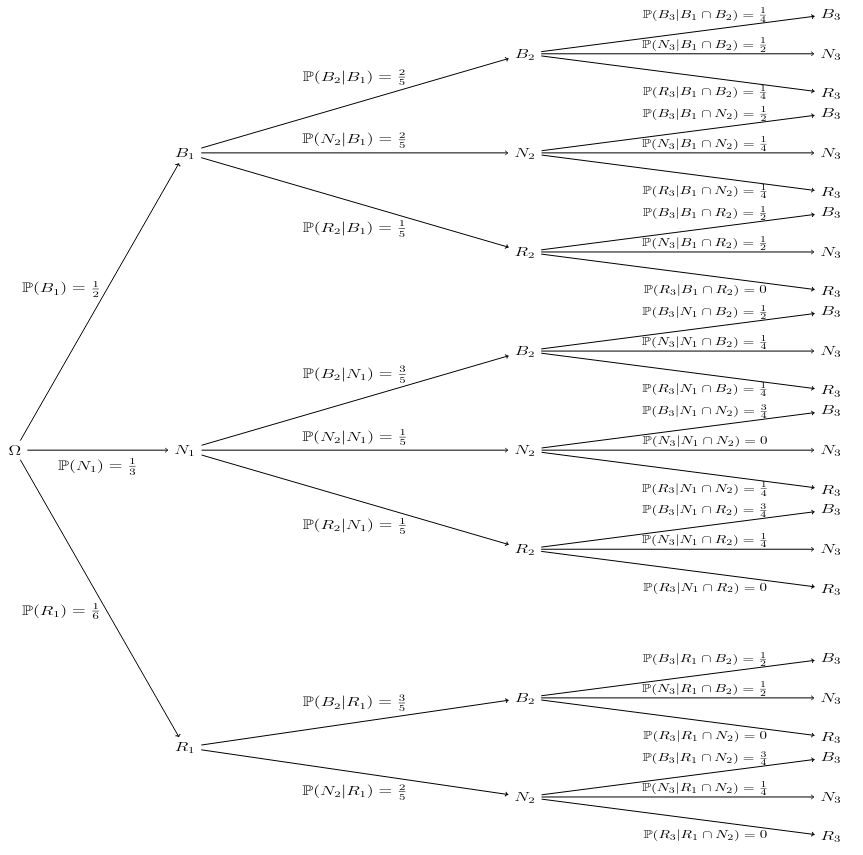
\includegraphics[width=0.75\linewidth]{tree.png}
\end{figure}


\newpage

\section{Calcolo combinatorio e spazi di probabilità finiti e uniformi}
\begin{itemize}
    \item $|A| = |B|$ se e solo se $A$ e $B$ sono in corrispondenza biunivoca.
    \item \textbf{fattoriale}: $ n! = n(n-1)\cdots 1, \quad \forall n=1,2,\dots; \quad ricorda:  0! = 1 $
    
    \item \textbf{coefficiente binomiale}:
    $$ \binom{n}{k} = \frac{n!}{k!(n-k)!}, \quad \forall n,k = 0,1,2,\dots \text{ con } k \le n. $$
    $$ \binom{n}{k} = \binom{n}{n-k} \quad \to \quad \binom{n}{0} = \binom{n}{n} = 1, \quad \binom{n}{1} = n. $$
    
    \item \textbf{formula di Stifel}:
    $$ \binom{n}{k} = \binom{n-1}{k-1} + \binom{n-1}{k} $$

    \item \textbf{formula del binomio di Newton}:
    $$ (a+b)^n = \sum_{k=0}^{n} \binom{n}{k} a^k b^{n-k}, \quad a,b \in \mathbb{R} $$

    \vspace{0.3cm}

    \item \textbf{metodo delle scelte successive}: Se devo scegliere tra x cose, successivamente tra x-1 cose, poi da x-2 cose... etc, per determinare la cardinalità farò: $|A| = x \cdot (x-1)  \cdot (x-2) \cdot \dots \cdot (1)$   \footnote{vedi esercizio 1.2 di questo capitolo. In questo esercizio nota una cosa importante: intanto nel primo punto hai 4 possibilità perché $\binom{4}{3}$ e hai 6 possibilità perché $\binom{4}{2}.$\\ Nel secondo punto non puoi usare la stessa strategia del primo in quanto essendo due coppie (quindi =) sono interscambiabili. Mentre una coppia e un tris (quindi diversi) non sono interscambiabili.}

    \vspace{0.3cm}
\end{itemize}

\subsection{Disposizioni e combinazioni  {\footnotesize di n elementi in k posti}}
Nota per non confondersi: $n$ è l'insieme delle opzioni tra cui si può scegliere. $k$ è il numero di decisioni che vengono prese.
\begin{itemize}
    \item \textbf{Disposizioni semplici} \footnote{esempio: 3 (k) estrazioni da una box di 5 (n) elementi. Le possibilità sono 5 (prima estr) $\cdot$ 4 (seconda estr) $\cdot$ 3 (terza estr)} :  $D_{n,k} = \underbrace{n \cdot (n-1) \cdot (n-2) \dots (n-k+1)}_{k \text{ volte}} =$ {\large $\frac{n!}{(n-k)!} \quad$} {\footnotesize (l'ordine conta)}

    \item \textbf{Disposizioni con ripetizioni} \footnote{esempio: devi riempire una password di 4 (k) caratteri con le 26 (n) lettere dell'alfabeto. Avrai dunque 26 combinazioni ciascun carattere, quindi 26 $\cdot$ 26 $\cdot$ 26 $\cdot$ 26 = $26^4$ combinazioni.}: $DR_{n,k} = n^{k}$ 

    \item \textbf{Permutazioni}: $P_n = n! = n \cdot (n-1) \cdot (n-2) \cdot \dots \cdot 1 = D_{n,n} \quad$ {\footnotesize (sostanzialmente è il fattoriale)}

    \item \textbf{Combinazioni semplici} \footnote{esempio: ho 3 (n) lettere che voglio mettere in una determinata combinazione (per esempio in ordine alfabetico). Questa combinazione contiene 3 (k) lettere. Ho quindi 6 disposizioni possibili: ABC, ACB, BCA, BAC, CAB, CBA. ma una sola combinazione corretta: ABC}: {\large $C_{n,k} =  \frac{n!}{(n-k)! \cdot k!} = \binom{n}{k} \quad$ } {\footnotesize (l'ordine NON conta)}

    \item \textbf{Combinazioni con ripetizioni} \footnote{ 5 palline rosse indistinguibili e 3 cassetti. In quanti modi posso combinare le palline nei 3 cassetti?}: {\large $C_{n,k} =  \frac{(n+k-1)!}{(n-1)! \cdot k!} = \binom{n+k-1}{k}$ } \\ {\footnotesize \textbf{Attenzione}: su questo spazio la probabilità \textbf{non} è uniforme, quindi non ci si può applicare Laplace. Con le ripetizioni conviene sempre usare $\Omega = DR_{n,k}$.}

    \item \textbf{Permutazioni con ripetizione} (anagrammi): se $n$ oggetti sono di $r$ tipi con molteplicità $n_1,\dots,n_r$ ($\sum n_i = n$), i modi distinti di ordinarli sono
    $$ \frac{n!}{n_1! \, n_2! \cdots n_r!} \quad \text{(coefficiente multinomiale)} $$
\end{itemize}

\vspace{0.4cm}
\subsection{Tabella riassuntiva: quale $\Omega$ scegliere}
Urna con $n$ palline, se ne estraggono $k$. \textbf{Prima cosa da chiedersi in ogni esercizio}: conta l'ordine? ci sono ripetizioni?
\begin{center}
\renewcommand{\arraystretch}{1.6}
\begin{tabular}{|l|c|c|}
\hline
\textbf{ORDINE / RIPETIZIONE} & \textbf{Senza ripetizione} & \textbf{Con ripetizione} \\ \hline
\textbf{Si tiene conto dell'ordine} & \begin{tabular}{@{}c@{}} Estrazione \textbf{senza reimmissione} \\ $\Omega = D_{n,k}$, \; $|\Omega| = \frac{n!}{(n-k)!}$ \end{tabular} & \begin{tabular}{@{}c@{}} Estrazione \textbf{con reimmissione} \\ $\Omega = DR_{n,k}$, \; $|\Omega| = n^k$ \end{tabular} \\ \hline
\textbf{Non si tiene conto dell'ordine} & \begin{tabular}{@{}c@{}} Estrazione \textbf{simultanea} \\ $\Omega = C_{n,k}$, \; $|\Omega| = \binom{n}{k}$ \end{tabular} & \begin{tabular}{@{}c@{}} \textit{(comb. con ripetizione:} \\ \textit{$\mathbb{P}$ non uniforme, evitare)} \end{tabular} \\ \hline
\end{tabular}
\end{center}
\begin{itemize}
    \item L'\textbf{estrazione simultanea} è un'estrazione senza reimmissione in cui l'ordine non conta: si può usare indifferentemente $\Omega = C_{n,k}$ oppure $\Omega = D_{n,k}$ (ad ogni combinazione corrispondono $k!$ disposizioni). \\ {\footnotesize Perciò \textbf{"senza reimmissione" e "simultanea" danno sempre lo stesso risultato}: basta essere coerenti (se conto l'ordine sopra, lo conto anche sotto).}
    \item $|C_{n,k}| \cdot |P_k| = |D_{n,k}|$ (dove $P_k = k!$ è il numero di permutazioni di $k$ elementi), cioè $\binom{n}{k} \cdot k! = \frac{n!}{(n-k)!}$.
\end{itemize}

\paragraph{Oggetti distinguibili o indistinguibili: cosa cambia davvero.}
Due oggetti sono \textbf{distinguibili} se scambiandoli di posto ottengo un esito \emph{diverso} (hanno un'identità: sono numerati, colorati diversamente, hanno un nome). Sono \textbf{indistinguibili} se scambiandoli ottengo lo \emph{stesso} esito (contano solo \emph{quanti} ce ne sono, non \emph{quali}).
\begin{itemize}
    \item \textbf{Test operativo}: prendo due oggetti e li scambio. Se l'esito cambia $\to$ distinguibili $\to$ conto le \textbf{sequenze} ($D$, $DR$). Se l'esito non cambia $\to$ indistinguibili $\to$ conto gli \textbf{insiemi}/le quantità ($C$, $CR$).
    \item {\footnotesize \textit{Es. 7 palle \textbf{numerate} in 3 scatole}: "palla 1 in scatola A, palla 2 in B" $\ne$ "palla 1 in B, palla 2 in A" $\to$ distinguibili $\to \Omega = DR_{3,7}$. Se invece le 7 palle fossero identiche, i due esiti sarebbero lo stesso $\to CR_{3,7}$.}
    \item {\footnotesize \textit{Es. estrazione di 5 carte}: le carte sono sempre distinguibili tra loro; è l'\textbf{ordine di estrazione} che posso scegliere di ignorare ($C_{40,5}$) o no ($D_{40,5}$).}
\end{itemize}
\textbf{Attenzione, i due concetti si confondono facilmente}: "distinguibili" riguarda gli \textbf{oggetti}, "conta l'ordine" riguarda le \textbf{posizioni}. Nella pratica vanno insieme: oggetti distinguibili $\to$ righe della tabella con l'ordine; oggetti indistinguibili $\to$ righe senza ordine.
\begin{itemize}
    \item \textbf{Regola d'oro per gli esercizi}: se il testo dice \emph{"a caso"}, \emph{"in modo casuale"}, \emph{"equiprobabile"}, allora \textbf{devi} rendere gli oggetti distinguibili (numerarli mentalmente) e usare $D$/$DR$/$C$. \\ {\footnotesize Motivo: le configurazioni di oggetti \emph{indistinguibili} ($CR_{n,k}$) \textbf{non} sono equiprobabili — "2 palline nella scatola 1" si realizza in molti più modi di "tutte e 5 nella scatola 1" — quindi su quello spazio Laplace ($\frac{|A|}{|\Omega|}$) darebbe risultati sbagliati.}
    \item \textbf{Le palline indistinguibili possono comunque comparire}: quando è l'\emph{evento} (non lo spazio) a ignorare l'identità. {\footnotesize Es.: $\Omega = DR_{3,7}$ (distinguibili), ma l'evento "2 palle nella scatola 1 e 3 nella scatola 2" si conta con $\binom{7}{2}\binom{5}{3}$, cioè scegliendo \emph{quali} palle senza ordinarle.}
\end{itemize}

\begin{table}[htbp]
\centering
{\footnotesize \textbf{Chi è $n$ e chi è $k$?} $\;n=$ \textbf{quante alternative} ho ad ogni scelta (l'insieme da cui pesco: facce, numeri, carte, \emph{scatole}); $k=$ \textbf{quante scelte} faccio (estrazioni, lanci, \emph{palline} da collocare, posizioni da riempire). In $n^k$: la \textbf{base} sono le alternative, l'\textbf{esponente} le prove. Nei problemi urne/scatole è il punto in cui si sbaglia: $n=$ scatole, $k=$ palline, mai il contrario.}
\vspace{0.15cm}
\renewcommand{\arraystretch}{1.5}
\begin{tabular}{|p{2.2cm}|p{6.4cm}|p{6.4cm}|}
\hline
\textbf{ORDINE / RIPETIZIONE} & \textbf{Senza ripetizione} & \textbf{Con ripetizione} \\
\hline
\textbf{Si tiene conto dell'ordine} &
\textbf{Estrazione senza reimmissione}\newline
$\Omega = D_{n,k}, \quad |\Omega| = \frac{n!}{(n-k)!}$\newline
{\footnotesize
- Podio ordinato di 3 persone su 10: $n=10$ persone, $k=3$ posti.\newline
- 5 estrazioni senza reimmissione da un mazzo di 40 \emph{in cui conta l'ordine}: $\Omega=D_{40,5}$ ($n=40$ carte, $k=5$ estrazioni).\newline
- Caso $k=n$ (si estrae \emph{tutto}): $\Omega=$ permutazioni, $|\Omega|=n!$ (es. $n$ palline numerate estratte tutte senza reimmissione; 52 carte mescolate $\to 52!$).\newline
\textit{Urne/scatole}: 3 palline \textbf{distinguibili} in 10 scatole con \textbf{max 1 pallina per scatola} ($n=10$ scatole, $k=3$ palline).} &
\textbf{Estrazione con reimmissione}\newline
$\Omega = DR_{n,k}, \quad |\Omega| = n^k$\newline
{\footnotesize
- 4 lanci di un dado a 6 facce: $n=6$ facce, $k=4$ lanci.\newline
- Schedina totocalcio: $n=3$ esiti, $k=13$ partite.\newline
- 5 estrazioni \emph{con} reimmissione da un mazzo di 40: $\Omega=DR_{40,5}$.\newline
\textit{Urne/scatole} (caso più frequente): 7 palle \textbf{numerate} ripartite a caso in 3 scatole $\to \Omega=DR_{3,7}=3^7$ ($n=3$ scatole, $k=7$ palle); 5 palline in 3 urne $\to 3^5$. \textbf{Non} $7^3$: ogni pallina è una scelta con 3 alternative.} \\
\hline
\textbf{Non si tiene conto dell'ordine} &
\textbf{Estrazione simultanea}\newline
$\Omega = C_{n,k}, \quad |\Omega| = \binom{n}{k}$\newline
{\footnotesize
- Superenalotto, 6 numeri distinti da 1 a 90: $\Omega=C_{90,6}$ ($n=90$ numeri, $k=6$ estratti).\newline
- 2 lupi assegnati a caso tra 10 giocatori: $\Omega=C_{10,2}$ ($n=10$ giocatori, $k=2$ ruoli uguali).\newline
- 5 carte senza reimmissione da un mazzo di 40, l'ordine \emph{non} conta: $\Omega=C_{40,5}$.\newline
\textit{Urne/scatole}: scegliere 3 scatole (su 10) in cui piazzare 1 pallina indistinguibile.} &
\textit{(Comb. con ripetizione: $\mathbb{P}$ non uniforme, evitare)}\newline
$\Omega = CR_{n,k}, \quad |\Omega| = \binom{n+k-1}{k}$\newline
{\footnotesize
- Distribuire $k$ palline \textbf{indistinguibili} in $n$ urne ($n=$ urne, $k=$ palline).\newline
\textit{Attenzione}: gli esiti \textbf{non} sono equiprobabili, non si può usare Laplace. Se il testo dice \emph{"a caso"}, rendi le palline distinguibili e usa $DR_{n,k}$.} \\
\hline
\end{tabular}
\end{table}


\vspace{0.4cm}
\subsubsection{Metodo delle scelte successive: enunciato e trappole}
Se ogni elemento di $A$ si determina tramite \textbf{una e una sola} sequenza di $k$ scelte successive, con $n_1, n_2, \dots, n_k$ possibilità (ogni $n_i$ fissato, non dipendente dalle scelte precedenti), allora
$$ |A| = n_1 \cdot n_2 \cdots n_k $$
\textbf{I due errori tipici:}
\begin{itemize}
    \item \textbf{non contare tutti} gli elementi di $A$ (da qui "ciascun");
    \item \textbf{contare più volte} lo stesso elemento (da qui "una e una sola") $\to$ \textbf{sovra-conteggio}.
\end{itemize}
\textbf{Regola anti-sovra-conteggio}: se scelgo in sequenza $m$ gruppi \textbf{dello stesso tipo} (quindi interscambiabili), sto contando ogni configurazione $m!$ volte $\to$ devo dividere per $m!$, oppure (meglio) scegliere i loro tipi \textbf{insieme} con una combinazione.
\begin{eserciziobox}{{Full vs Doppia coppia (mazzo da poker da 52 carte)}}
\textbf{Full} (un tris + una coppia, di tipi diversi): tris e coppia sono \textbf{ruoli diversi}, quindi NON interscambiabili $\to$ scelte successive dirette:
$$ |A| = \underbrace{13}_{\text{tipo tris}} \cdot \underbrace{12}_{\text{tipo coppia}} \cdot \underbrace{\binom{4}{3}}_{\text{semi tris}} \cdot \underbrace{\binom{4}{2}}_{\text{semi coppia}} = 13 \cdot 12 \cdot 4 \cdot 6 = 3744 $$

\textbf{Doppia coppia} (due coppie + una quinta carta): le due coppie sono \textbf{lo stesso ruolo} $\to$ interscambiabili!
$$ 13 \cdot 12 \cdot 11 \cdot 6 \cdot 6 \cdot 4 = 247104 \quad \text{\textbf{SBAGLIATO}: ogni mano contata } 2! = 2 \text{ volte} $$
$$ |B| = \frac{247104}{2} = 123552 \qquad \text{oppure, direttamente: } \underbrace{\binom{13}{2}}_{78} \cdot \underbrace{11}_{\text{5\textsuperscript{a} carta}} \cdot 6 \cdot 6 \cdot \underbrace{4}_{\text{suo seme}} = 123552 $$
\textit{Morale}: se i gruppi scelti sono \textbf{uguali tra loro} (2 coppie, 2 mazzi da 20, ecc.) $\to$ combinazione o divisione per il fattoriale. Se sono \textbf{diversi} (un tris e una coppia) $\to$ scelte successive normali.
\end{eserciziobox}

\subsubsection{Distribuzione binomiale}
Si usa dove si effettuano $n$ estrazioni \textbf{con reimmissione} (prove \textbf{indipendenti}: per questo le probabilità delle varie estrazioni si possono moltiplicare). Per esempio: \textit{si calcoli la probabilità di ottenere 2 palline rosse estraendone (con reimmissione) 4 da un’urna che contiene 3 palline rosse e 7 bianche}.\\ Devo calcolare $A_k =$ "si estraggono $k$=2 palline rosse ed $n-k=4-2$ palline bianche" (con $0 \le k \le n$).
$$\Omega = DR_{b+r,n} \quad \quad \mathbb{P}(A_k) = {\binom{n}{k} \cdot p^k \cdot(1-p)^{n-k}}$$
Dove:
\begin{itemize}
    \item $n$: numero totale di prove/estrazioni. {\footnotesize =4}
    \item $k$: numero di successi desiderati. {\footnotesize ( =2, ovvero quante palline rosse vogliamo estrarre)}
    \item $p$: probabilità di successo in una singola prova. {\footnotesize (in questo caso: $p = \frac{r}{b+r}$ = probabilità di estrarre una pallina rossa in una singola estrazione)}
    \item $(1 - p)$: probabilità di insuccesso
    \item $\binom{n}{k}$: coefficiente binomiale, calcolato come $\frac{n!}{k!(n-k)!}$.
\end{itemize}


\subsubsection{Distribuzione Ipergeometrica}
Questa si utilizza invece con estrazioni \textbf{senza reimmissione \footnote{formula più semplice (con la notazione qui sotto): $\frac{\binom{n}{k} \cdot [K(K-1)\cdots(K-k+1)] \cdot [(N-K)(N-K-1)\cdots(N-K-(n-k)+1)]}{N(N-1)(N-2)\cdots(N-n+1)}$; es.: $\frac{\binom{4}{2} \cdot 3 \cdot 2 \cdot 7 \cdot 6}{10 \cdot 9 \cdot 8 \cdot 7}$}} o \textbf{simultanee}. Con l'esempio precedente:
$$\mathbb{P}(A_k) = \frac{\binom{K}{k} \cdot \binom{N - K}{n - k}}{\binom{N}{n}}$$
Dove: 
\begin{itemize}
    \item $N$: numero totale di elementi nella popolazione {\footnotesize (= 10 = totale palline nell'urna)}
    \item $K$: numero totale di elementi "successo" disponibili nella popolazione {\footnotesize (= 3 = numero di palline disponibili del colore rosso)}
    \item $n$: numero di elementi estratti. {\footnotesize (= n precedente)}
    \item $k$: numero di successi desiderati. {\footnotesize (= k precedente)}
    \item $N - K$: numero di elementi "insuccesso" nella popolazione {\footnotesize (= 7 = numero di palline di altro colore (bianco))}
    \item $n - k$: numero di insuccessi nel campione {\footnotesize (= 2 = numero delle palline bianche da estrarre)}
\end{itemize}
Nell'esempio sopra hai che:
\begin{itemize}[-]
    \item $\binom{K}{k}$ = in quanti modi posso scegliere 2 rosse dalle 3 disponibili = $\binom{3}{2} = 3$ = (modi di scegliere le rosse). 
    \item $\binom{N-K}{n-k}$ = in quanti modi posso scegliere 2 bianche dalle 7 disponibili = $\binom{7}{2} = 21$ (modi di scegliere le bianche)
    \item $\binom{N}{n}$ = tutti i modi possibili di scegliere 4 palline da 10 = $\binom{10}{4} = 210$ (casi totali)
\end{itemize}

\vspace{0.3cm}
\textbf{Equivalenza binomiale/ipergeometrica nei tre schemi} (urna con $b$ bianche, $r$ rosse, $N = b+r$; $k$ estrazioni, $l$ successi):
\begin{itemize}[-]
    \item \textbf{con reimmissione}: $\displaystyle \frac{\binom{k}{l} \cdot b^l \cdot r^{k-l}}{N^k} = \binom{k}{l} p^l (1-p)^{k-l}$ \quad con $p = \frac{b}{N}$
    \item \textbf{senza reimmissione}: $\displaystyle \frac{\binom{k}{l} \cdot [b(b-1)\cdots] \cdot [r(r-1)\cdots]}{N(N-1)\cdots(N-k+1)}$ \quad {\footnotesize (al numeratore $l$ fattori decrescenti da $b$ e $k-l$ da $r$)}
    \item \textbf{simultanea}: $\displaystyle \frac{\binom{b}{l}\binom{r}{k-l}}{\binom{N}{k}}$
\end{itemize}
{\footnotesize \textbf{Senza reimmissione e simultanea danno sempre lo stesso numero}; solo la reimmissione cambia il risultato.}

\vspace{0.5cm}
\subsection{Schemi ricorrenti negli esercizi}
\begin{itemize}
    \item \textbf{Indovinare al primo tentativo} una sequenza di $k$ simboli scelti fra $n$: $\mathbb{P} = \frac{1}{n^k}$. \\ {\footnotesize Es. combinazione di 6 cifre: $10^{-6}$; di 6 lettere fra X,Y,Z,W: $4^{-6}$.}

    \item \textbf{Indovinare i primi $k$ classificati} su $n$ concorrenti: \\
    con l'ordine (podio ordinato): $\mathbb{P} = \frac{1}{D_{n,k}} = \frac{(n-k)!}{n!}$ \\
    senza l'ordine (solo i nomi): $\mathbb{P} = \frac{1}{C_{n,k}} = \frac{1}{\binom{n}{k}} = \frac{k!}{D_{n,k}}$

    \item \textbf{$m$ persone scelgono fra $n$ opzioni} (indipendentemente): $|\Omega| = n^m$. \\
    \emph{tutte la stessa opzione}: $\frac{n}{n^m}$; \quad \emph{tutte opzioni diverse}: $\frac{D_{n,m}}{n^m} = \frac{n(n-1)\cdots(n-m+1)}{n^m}$.

    \item \textbf{Una carta specifica è nella mano}: pescando $n$ carte da un mazzo di $N$,
    $$ \mathbb{P}(\text{quella carta c'è}) = \frac{\binom{N-1}{n-1}}{\binom{N}{n}} = \frac{n}{N} $$
    Più in generale, $j$ carte fissate sono \textbf{tutte} nella mano:
    $$ \mathbb{P} = \frac{\binom{N-j}{n-j}}{\binom{N}{n}} = \frac{n(n-1)\cdots(n-j+1)}{N(N-1)\cdots(N-j+1)} $$
    {\footnotesize Es. 10 carte su 40: l'asso di bastoni c'è con prob. $10/40 = 25\%$; asso di spade \emph{e} asso di coppe con prob. $\frac{10 \cdot 9}{40 \cdot 39} = \frac{3}{52} \approx 5.77\%$.}

    \item \textbf{Divisione in due mazzi/gruppi}: dividere $N$ carte in due mazzi da $N/2$ $\to$ $\Omega = C_{N,N/2}$ (basta descrivere il primo mazzo, il secondo è determinato). \\ {\footnotesize Es. "il primo mazzo da 20 (su 40) contiene esattamente un 7": scelgo quale dei 4 sette ($4$ modi) e le altre 19 carte fra le 36 non-sette: $\mathbb{P} = \frac{4\binom{36}{19}}{\binom{40}{20}} = \frac{120}{481} \approx 25\%$.}

    \item \textbf{Almeno una coincidenza} (paradosso dei compleanni): $n$ persone, $N = 365$ giorni. Si passa al complementare "tutti diversi":
    $$ p_n = 1 - \frac{D_{365,n}}{365^n} = 1 - \frac{\prod_{i=0}^{n-1}(365-i)}{365^n} $$
    {\footnotesize $p_n > \frac{1}{2} \iff n \ge 23$. Schema generale: "almeno due uguali" $= 1 - \frac{D_{N,n}}{N^n}$.}

    \item \textbf{Schedina / griglia con doppie} (Totocalcio): $13$ partite, $3$ esiti $\to |\Omega| = 3^{13}$. Giocando una doppia per partita si coprono $2^{13}$ colonne.
    $$ \mathbb{P}(13) = \frac{2^{13}}{3^{13}}, \qquad \mathbb{P}(12) = \frac{2^{12} \cdot 13}{3^{13}} $$
    {\footnotesize ($12$: sbaglio esattamente una partita, $13$ scelte su quale, e su quella l'esito giusto è l'unico non coperto dalla doppia $\to$ $1$ modo; sulle altre 12 partite $2$ scelte ciascuna.)}

    \item \textbf{Estrazione con numero jolly} (Superenalotto, "5+1"): estratti $6$ numeri su $90$ + un $7^\circ$ jolly diverso dai precedenti. Si conta su $\Omega = D_{90,7}$: scelgo quale dei $6$ numeri giocati manca ($6$ modi), i restanti $5$ vanno nei $6$ posti in $6!/1!$ ordinamenti e il jolly è il numero mancante.

    \item \textbf{Mani di poker} (5 carte su 52, $|\Omega| = \binom{52}{5} = 2\,598\,960$): \\
    \begin{tabular}{@{}ll@{}}
    scala reale massima & $4$ \\
    scala reale (qualsiasi, stesso seme) & $4 \cdot 10 = 40$ \\
    scala (semi qualsiasi) & $10 \cdot 4^5 - 40 = 10\,200$ \; {\footnotesize (senza togliere le scale reali: $10\,240$)} \\
    colore (5 dello stesso seme) & $4\binom{13}{5} = 5\,148$ \\
    poker (4 dello stesso tipo) & $13 \cdot 48 = 624$ \\
    full (tris + coppia) & $13 \cdot 12 \cdot 4 \cdot 6 = 3\,744$ \\
    tris (esattamente) & $13\binom{4}{3}\binom{12}{2}4^2 = 54\,912$ \\
    doppia coppia & $\binom{13}{2}\binom{4}{2}^2 \cdot 11 \cdot 4 = 123\,552$ \\
    coppia (esattamente) & $13\binom{4}{2}\binom{12}{3}4^3 = 1\,098\,240$ \\
    \end{tabular} \\
    {\footnotesize Schema: \textbf{prima i tipi} (con $\binom{13}{\cdot}$ o prodotti se i ruoli sono diversi), \textbf{poi i semi} dentro ogni tipo. La parola \textbf{"esattamente"} obbliga a scegliere i tipi restanti \textbf{distinti} tra loro (con $\binom{12}{2}$, $\binom{12}{3}$) e non con semplici prodotti.}
\end{itemize}





























\section{Variabili Aleatorie}

\subsection{Concetti Fondamentali}
\begin{itemize}
    \item \textbf{Variabile Aleatoria (v.a.):} Una funzione $X: \Omega \to \mathbb{R}$ che associa un numero reale a ogni esito dell'esperimento.
    \item \textbf{Evento generato da $X$:} $\{X \in B\} = \{\omega \in \Omega : X(\omega) \in B\}$. Rappresenta la condizione "il valore di $X$ appartiene all'insieme $B$".
    \item \textbf{Distribuzione (o Legge) $\mathbb{P}_X$:} Funzione che assegna probabilità ai sottoinsiemi di $\mathbb{R}$:
    \begin{equation*}
        \mathbb{P}_X(B) = \mathbb{P}(X \in B)
    \end{equation*}
\end{itemize}

\subsection{Notazione degli eventi generati}
Tutti gli eventi si riscrivono nella forma $\{X \in B\}$ con $B \subset \mathbb{R}$:
\begin{center}
\begin{tabular}{|l|l||l|l|}
\hline
$\{X \in \{x\}\}$ & $\{X = x\}$ & $\{X \in (x,y)\}$ & $\{x < X < y\}$ \\ \hline
$\{X \in (-\infty, x)\}$ & $\{X < x\}$ & $\{X \in [x,y)\}$ & $\{x \le X < y\}$ \\ \hline
$\{X \in (-\infty, x]\}$ & $\{X \le x\}$ & $\{X \in (x,y]\}$ & $\{x < X \le y\}$ \\ \hline
$\{X \in (x,+\infty)\}$ & $\{X > x\}$ & $\{X \in [x,y]\}$ & $\{x \le X \le y\}$ \\ \hline
$\{X \in [x,+\infty)\}$ & $\{X \ge x\}$ & $\{X \in \emptyset\} = \emptyset$ & $\{X \in \mathbb{R}\} = \Omega$ \\ \hline
\end{tabular}
\end{center}
\begin{itemize}
    \item \textbf{Eventi generati da una costante} $X = a$: solo $\Omega$ (se $a \in B$) oppure $\emptyset$ (se $a \notin B$).
    \item \textbf{Eventi generati da un'indicatrice} $X = 1_A$: solo $A$, $A^c$, $\Omega$, $\emptyset$.
    \\ {\footnotesize $\{X \in B\} = A$ se $1 \in B, 0 \notin B$; $= A^c$ se $0 \in B, 1 \notin B$; $= \Omega$ se entrambi in $B$; $= \emptyset$ se nessuno.}
    \item Un'indicatrice contiene tutta l'informazione dell'evento: la v.a. \textbf{generalizza} la nozione di evento.
\end{itemize}

\subsection{Casi Particolari Notevoli}
\begin{itemize}
    \item \textbf{v.a. Costante ($X = a$):} Assume sempre il valore $a$, $\implies$ $X(w)=a \hspace{1em}\forall w\in \Omega$
    \begin{itemize}
        \item \textit{Distribuzione:} $\mathbb{P}_X = \delta_a$ (Delta di Dirac in $a$).
        $$
        \mathbb{P}_X(B) = \mathbb{P}(X \in B) = \begin{cases}
            1 & a\in B \\
            0 & a \notin B
        \end{cases}
        $$
        
        \item \textit{CDF:} $F_X(x) = 1$ se $x \ge a$, altrimenti $0$.
    \end{itemize}
    \item \textbf{v.a. Indicatrice ($1_A$):} Vale $1$ se si verifica l'evento $A$, $0$ altrimenti $\implies$ $X(w) = \begin{cases}
        1 & w\in A \\ 0 & w\notin A
    \end{cases}$
    \begin{itemize}
        \item \textit{Distribuzione:} Bernoulli di parametro $p = \mathbb{P}(A) \implies (1-p)\delta_0 + p\delta_1$.
        $$
        \mathbb{P}_X(B) = \begin{cases}
            \mathbb{P}(A) & 1\in B \land 0\notin B \\
            \mathbb{P}(A^C) & 1\notin B \land 0\in B \\
            \mathbb{P}(\Omega) & 1\in B \land 0 \in B \\
            0 & 1\notin B  \land 0 \notin B
        \end{cases}
        =
        \begin{cases}
            \mathbb{P}(A) & 1\in B \land 0\notin B \\
            1-\mathbb{P}(A) & 1\notin B \land 0\in B \\
            1 & 1\in B \land 0 \in B \\
            0 & 1\notin B  \land 0 \notin B
        \end{cases}
        $$
        
        \item \textit{CDF:} 
        $F_X(x) = \begin{cases} 0 & x < 0 \\ 1-p & 0 \le x < 1 \\ 1 & x \ge 1 \end{cases}$
    \end{itemize}
\end{itemize}

\subsection{Funzione di Ripartizione (CDF)}
Definita come $F_X(x) = \mathbb{P}(X \le x)$. 
\paragraph{Proprietà Fondamentali:}
\begin{enumerate}
    \item \textbf{Monotonia:} $x \le y \implies F_X(x) \le F_X(y)$ (è non decrescente).
    \item \textbf{Limiti agli estremi:} $\lim_{x \to -\infty} F_X(x) = 0$ e $\lim_{x \to +\infty} F_X(x) = 1$.
    \item \textbf{Continuità a destra:} $\lim_{y \to x^+} F_X(y) = F_X(x)$.
    \item \textbf{Salto (Limite a sinistra):} $F_X(x^-) = \lim_{y \to x^-} F_X(y) = \mathbb{P}(X < x)$.
\end{enumerate}

\paragraph{Nota operativa:} $F_X$ è continua in $x \iff \mathbb{P}(X=x) = 0$. Se c'è un "salto", la v.a. ha una massa di probabilità in quel punto.

\paragraph{Teorema di caratterizzazione (vale anche il viceversa!):} se una funzione $G : \mathbb{R} \to [0,1]$ è \textbf{non decrescente}, \textbf{continua a destra}, con $\lim_{x\to-\infty} G = 0$ e $\lim_{x\to+\infty} G = 1$, allora esiste una v.a. $X$ tale che $G = F_X$. \\ {\footnotesize Serve negli esercizi del tipo "stabilire se la funzione data può essere una funzione di ripartizione": basta verificare le 4 proprietà. Conoscere $F_X$ equivale a conoscere tutta la legge $\mathbb{P}_X$.}

\newpage
\subsection{Calcolo delle Probabilità su Intervalli}
Utilizzare le seguenti formule per risolvere gli esercizi basati sulla CDF ($F_X$):

\begin{center}
\renewcommand{\arraystretch}{1.5}
\begin{tabular}{|l|l|l|}
\hline
\textbf{Evento} & \textbf{Formula con CDF} & \textbf{Spiegazione intuitiva} \\ \hline
$\mathbb{P}(X = x)$ & $F_X(x) - F_X(x^-)$ & Valore del "salto" in $x$ \\ \hline
$\mathbb{P}(X > x)$ & $1 - F_X(x)$ & Complementare di $\{X \le x\}$ \\ \hline
$\mathbb{P}(X < x)$ & $F_X(x^-)$ & Limite da sinistra in $x$ \\ \hline
$\mathbb{P}(a < X \le b)$ & $F_X(b) - F_X(a)$ & Probabilità standard tra due punti \\ \hline
$\mathbb{P}(a \le X \le b)$ & $F_X(b) - F_X(a^-)$ & Include il punto $a$ (usa il limite sx) \\ \hline
$\mathbb{P}(a \le X < b)$ & $F_X(b^-) - F_X(a^-)$ & Esclude $b$, include $a$ \\ \hline
$\mathbb{P}(a < X < b)$ & $F_X(b^-) - F_X(a)$ & Esclude entrambi gli estremi \\ \hline
\end{tabular}
\end{center}

\subsection{Relazioni Utili}
\begin{itemize}
    \item \textbf{Additività:} $\mathbb{P}(X \le x) = \mathbb{P}(X < x) + \mathbb{P}(X = x)$.
    \item \textbf{Stabilità per limiti:} Se $A_n \uparrow A$, allora $\mathbb{P}(A_n) \to \mathbb{P}(A)$. Utile per dimostrare i limiti della CDF.
\end{itemize}

\newpage
\subsection{Le tre "specie" di variabili aleatorie: discreta, continua, MISTA}
Non tutte le v.a.\ sono o discrete o continue: esiste il caso \textbf{misto}, e all'esame viene chiesto spesso (\emph{"si mostri che $X$ non è assolutamente continua"}, \emph{"si verifichi che la legge di $Z$ non è né continua né discreta"}). La distinzione si legge \textbf{tutta} sulla forma di $F_X$:

\begin{center}
\renewcommand{\arraystretch}{1.7}
\small
\begin{tabular}{|l|l|l|}
\hline
\textbf{Tipo} & \textbf{Com'è fatta $F_X$} & \textbf{Come si descrive la legge} \\ \hline
\textbf{Discreta} & \emph{a gradini}: costante a tratti, sale solo con salti & densità discreta $p_X(x_i) = \mathbb{P}(X = x_i)$ \\ \hline
\textbf{Assol. continua} & \emph{continua ovunque}, nessun salto & densità $f_X = F_X'$, e $\mathbb{P}(X = x) = 0\;\forall x$ \\ \hline
\textbf{Mista} & continua a tratti, \textbf{ma con almeno un salto} & atomi $+$ densità (vedi sotto) \\ \hline
\end{tabular}
\end{center}

\paragraph{Il criterio operativo (l'unica cosa da guardare).} Il salto di $F_X$ nel punto $x_0$ \textbf{è} la massa concentrata lì:
$$ \boxed{\;\mathbb{P}(X = x_0) = F_X(x_0) - F_X(x_0^-)\;} $$
\begin{itemize}
    \item Se \textbf{esiste un salto} $\Rightarrow$ $X$ \textbf{non è assolutamente continua} (c'è un punto con probabilità positiva, mentre una v.a.c.\ ha $\mathbb{P}(X=x)=0$ per ogni $x$). \\ {\footnotesize Questo è \emph{tutto} quello che serve scrivere quando l'esercizio chiede "si mostri che $X$ non è assolutamente continua per alcun valore del parametro": si esibisce il salto e si osserva che è $>0$.}
    \item Se \textbf{oltre al salto} $F_X$ cresce anche con continuità su qualche intervallo $\Rightarrow$ $X$ \textbf{non è nemmeno discreta} (una discreta è \emph{costante} fra un salto e l'altro), quindi è \textbf{mista}.
\end{itemize}

\paragraph{Come si scrive (e si usa) una legge mista.} Si spezza in due pezzi, uno per gli atomi e uno per la parte con densità:
$$ \mathbb{P}_X = \underbrace{\sum_i p_i\, \delta_{x_i}}_{\text{parte discreta (i salti)}} \; + \; \underbrace{f_X \,dx}_{\text{parte continua}}, \qquad \text{con} \quad \sum_i p_i \;+\; \int_{-\infty}^{+\infty} f_X(x)\,dx = 1 $$
dove $f_X$ è la derivata di $F_X$ \textbf{là dove $F_X$ è derivabile}. Tutti i conti si fanno sommando i due contributi:
$$ \mathbb{E}[X] = \sum_i x_i\, p_i \; + \; \int x\, f_X(x)\,dx, \qquad \mathbb{E}[h(X)] = \sum_i h(x_i)\, p_i \; + \; \int h(x)\, f_X(x)\,dx $$
{\footnotesize \textbf{Attenzione ai simboli di disuguaglianza}: con una legge mista $\mathbb{P}(X < x_0) \ne \mathbb{P}(X \le x_0)$ nei punti-atomo. Usa la tabella "Calcolo delle Probabilità su Intervalli" qui sopra, che è scritta apposta con $F_X(x^-)$.}

\begin{eserciziobox}{{Esempio: riconoscere una legge mista da $F_X$}}
\textbf{Testo:} $F_X(x) = 0$ per $x<0$, \; $F_X(x) = \lambda x$ per $0 \le x < 1$, \; $F_X(x) = 1$ per $x \ge 1$, con $\lambda \in (0,1)$ fissato. Mostrare che $X$ non è assolutamente continua e calcolarne media.
\par\textbf{Soluzione:}
\begin{enumerate}
    \item \textbf{Il salto}: $F_X(1) = 1$ mentre $F_X(1^-) = \lambda$, quindi
    $$ \mathbb{P}(X = 1) = 1 - \lambda > 0 \qquad (\text{perché } \lambda < 1) $$
    Una v.a.\ assolutamente continua ha $\mathbb{P}(X = x) = 0$ per ogni $x$: quindi $X$ \textbf{non} lo è, per nessun $\lambda \in (0,1)$.
    \item \textbf{Non è nemmeno discreta}: su $[0,1)$ la $F_X$ cresce con continuità (pendenza $\lambda$), non a gradini. Quindi $X$ è \textbf{mista}.
    \item \textbf{Le due parti}: un atomo in $1$ di massa $1-\lambda$, e densità $f_X(x) = F_X'(x) = \lambda$ su $(0,1)$. \\ Verifica: $(1-\lambda) + \int_0^1 \lambda\,dx = (1-\lambda) + \lambda = 1$ \checkmark
    \item \textbf{Media}: $\;\mathbb{E}[X] = \underbrace{1 \cdot (1-\lambda)}_{\text{atomo}} + \underbrace{\int_0^1 x\,\lambda\,dx}_{\text{parte continua}} = 1 - \lambda + \frac{\lambda}{2} = \mathbf{1 - \frac{\lambda}{2}}$
\end{enumerate}
\end{eserciziobox}

\paragraph{La fabbrica principale di leggi miste: il TRONCAMENTO $Y = \min(X, c)$.} Compare ogni volta che il testo dice \emph{"lo strumento va fuori scala oltre $c$"}, \emph{"il rimborso è al massimo $c$"}, \emph{"si smette di aspettare dopo $c$ minuti"}. Con $X$ \textbf{continua}:
\begin{itemize}
    \item \textbf{Supporto}: $Y$ non può superare $c$, quindi $\mathcal{S}_Y \subseteq (-\infty, c]$.
    \item \textbf{CDF}: \; $F_Y(y) = F_X(y)$ per $y < c$, \; e $F_Y(y) = 1$ per $y \ge c$. {\footnotesize (Sotto la soglia $Y$ coincide con $X$; sopra, è già tutto accumulato.)}
    \item \textbf{L'atomo} si forma \textbf{nella soglia}, e vale tutta la coda schiacciata:
    $$ \boxed{\;\mathbb{P}(Y = c) = \mathbb{P}(X \ge c) = 1 - F_X(c)\;} $$
    \item \textbf{Media} (con la legge dello statistico inconscio, senza ricavare la legge di $Y$):
    $$ \mathbb{E}[Y] = \mathbb{E}[\min(X,c)] = \int_{-\infty}^{c} x\, f_X(x)\,dx \;+\; c \cdot \mathbb{P}(X \ge c) $$
    \item \textbf{Analogo} $Y = \max(X, c)$: l'atomo si forma sempre in $c$ ma raccoglie la coda \emph{sinistra}, $\mathbb{P}(Y = c) = \mathbb{P}(X \le c) = F_X(c)$, e la densità sopravvive su $(c, +\infty)$.
\end{itemize}
{\footnotesize \textbf{Confronto con il caso discreto} (v.\ §Trasformazioni di Variabili discrete): il meccanismo è identico, "la coda si accumula nell'ultimo punto". La differenza è che se $X$ è discreta anche $Y$ resta discreta, mentre se $X$ è continua $Y$ diventa \textbf{mista}: densità sotto la soglia $+$ un atomo esattamente sulla soglia. \\
\textbf{Caso limite da non farsi sfuggire}: se la soglia $c$ sta \textbf{sotto} tutto il supporto di $X$, allora $\min(X,c) = c$ sempre: $Y$ è \textbf{costante} (v.a.\ degenere, $\mathbb{P}(Y=c)=1$), non c'è più nessuna parte continua.}

\begin{eserciziobox}{{Esempio: strumento che va fuori scala (troncamento)}}
\textbf{Testo:} il tempo $T$ ha densità $f_T(t) = \frac32 t^2$ su $[0,1)$, $\;f_T(t) = a e^{-3(t-1)}$ per $t \ge 1$, $\;0$ altrimenti. Lo strumento misura esattamente $T$ solo se $T \le 1$; oltre va fuori scala e mostra sempre il valore $1$. Calcolare il valore atteso della misurazione.
\par\textbf{Soluzione:}
\begin{enumerate}
    \item \textbf{Costante $a$} (normalizzazione): $\int_0^1 \frac32 t^2 dt + \int_1^{+\infty} a e^{-3(t-1)} dt = \frac12 + \frac{a}{3} = 1 \implies \mathbf{a = \frac32}$.
    \item \textbf{La misurazione è} $M = \min(T, 1)$: legge mista, con atomo in $1$ di massa
    $$ \mathbb{P}(M = 1) = \mathbb{P}(T \ge 1) = \int_1^{+\infty} \tfrac32 e^{-3(t-1)}dt = \tfrac12 $$
    \item \textbf{Valore atteso} (parte continua $+$ atomo):
    $$ \mathbb{E}[M] = \int_0^1 t \cdot \tfrac32 t^2\,dt + 1\cdot\tfrac12 = \tfrac32 \cdot \tfrac14 + \tfrac12 = \tfrac38 + \tfrac12 = \mathbf{\tfrac78} $$
\end{enumerate}
{\footnotesize Confronta con $\mathbb{E}[T] = \int_0^1 \frac32 t^3 dt + \int_1^{+\infty} t\,\frac32 e^{-3(t-1)}dt = \frac38 + \frac12\big(1 + \frac13\big) = \frac38 + \frac23 = \frac{25}{24} > \frac78$: lo strumento \textbf{sottostima}, come è ovvio visto che taglia le code lunghe.}
\end{eserciziobox}

\begin{eserciziobox}{{Esempio: due troncamenti, uno "vero" e uno degenere}}
\textbf{Testo:} $X \sim Unif(a,b)$ con $\mathbb{E}[X] = 20$ e $\mathrm{Var}(X) = 12$. Trovare le leggi di $Y = \min(X, 20)$ e $Z = \min(X, 10)$.
\par\textbf{Soluzione:}
\begin{enumerate}
    \item \textbf{Ricavare $a$ e $b$}: $\frac{a+b}{2} = 20$ e $\frac{(b-a)^2}{12} = 12 \implies b-a = 12$. Quindi $\mathbf{a = 14},\ \mathbf{b = 26}$, con $f_X = \frac{1}{12}$ su $(14,26)$.
    \item \textbf{$Y = \min(X,20)$}: la soglia \textbf{cade dentro} il supporto $\Rightarrow$ legge \textbf{mista}. \\
    Atomo: $\mathbb{P}(Y = 20) = \mathbb{P}(X \ge 20) = \frac{26-20}{12} = \frac12$; \; densità $\frac{1}{12}$ su $(14,20)$ (che pesa l'altro $\frac12$).
    \item \textbf{$Z = \min(X,10)$}: la soglia sta \textbf{sotto} tutto il supporto ($X > 14 > 10$ sempre) $\Rightarrow$ $Z = 10$ con probabilità $1$: v.a.\ \textbf{degenere}, non mista. \\ {\footnotesize Prima di lanciarsi nei conti, guarda sempre \textbf{dove cade la soglia rispetto al supporto}: sopra, dentro, o sotto.}
\end{enumerate}
\end{eserciziobox}




\newpage
\section{Variabili Aleatorie Discrete (v.a.d.)}

\subsection{Definizioni di Base e Densità}
\begin{itemize}
    \item \textbf{v.a. discreta:} Una variabile che può assumere solo valori isolati (finiti o numerabili), come i risultati di un conteggio\footnote{Esempio: il numero di teste in 10 lanci di una moneta è una v.a. discreta ($S_X = \{0, 1, \dots, 10\}$), mentre l'altezza di una persona è continua.}.
    \item \textbf{Densità discreta (PMF):} $p_X(x) = \mathbb{P}(X = x)$. Indica la probabilità "puntuale" di ogni valore.
    \begin{itemize}
        \item \textit{Vincolo fondamentale:} $\sum_{i} p_X(x_i) = 1$. Se la somma non fa 1, non è una distribuzione valida\footnote{In un esercizio tipico: "Trova $k$ affinché $p_X(x) = k \cdot x$ sia una densità". Devi imporre $\sum k x_i = 1$ e risolvere per $k$.}.
        \item \textit{Vincolo fondamentale:} ogni densità discreta dev'essere compresa tra 0 e 1 (è una probabilità).
    \end{itemize}
    \item \textbf{Supporto $\mathcal{S}_X$:} L'elenco dei valori $x$ che hanno probabilità maggiore di zero.
\end{itemize}

\subsection{Calcolo delle Probabilità e CDF}
\begin{itemize}
    \item \textbf{Probabilità di un intervallo:} Per calcolare $\mathbb{P}(X \in B)$, somma semplicemente le probabilità dei valori del supporto che cadono dentro $B$\footnote{Esempio: Se $S_X = \{1, 2, 3, 4\}$ con probabilità uniformi, $\mathbb{P}(1.5 < X \le 3) = p_X(2) + p_X(3) = 1/4 + 1/4 = 1/2$.}.
    \item \textbf{Funzione di Ripartizione ($F_X$):} È una funzione "a gradini".
    \begin{itemize}
        \item Il valore di $F_X(x)$ "salta" verso l'alto ogni volta che $x$ tocca un valore del supporto.
        \item L'altezza del salto nel punto $x_i$ è esattamente $p_X(x_i)$\footnote{Se vedi un grafico della CDF che passa da 0.4 a 0.7 nel punto $x=2$, allora sai immediatamente che $\mathbb{P}(X=2) = 0.3$.}.
    \end{itemize}
\end{itemize}

\subsection{Indici di Sintesi: Media e Varianza}
\begin{itemize}
    \item \textbf{Media (Valore Atteso) $\mathbb{E}[X]$:} La media pesata dei valori.
    \begin{equation*}
        \mathbb{E}[X] = \sum x_i p_X(x_i)
    \end{equation*}
    \item \textbf{Linearità (Fondamentale per gli esercizi):} $\mathbb{E}[aX + b] = a\mathbb{E}[X] + b$\footnote{Esempio: Se sai che la media dei voti è 24 e il prof aggiunge 2 punti a tutti, la nuova media è $24+2=26$. Se raddoppia i voti, la media diventa 48.}.
    \item \textbf{Varianza $\mathrm{Var}(X)$:} Indica quanto i dati sono "sparpagliati" attorno alla media.
    \begin{itemize}
        \item \textit{Formula rapida:} $\mathrm{Var}(X) = \mathbb{E}[X^2] - (\mathbb{E}[X])^2$.
        \item \textit{Se indipendenti:} $\mathrm{Var}(X + Y) = \mathrm{Var}(X) + \mathrm{Var}(Y)$. {\footnotesize Se NON sono indipendenti serve il termine extra $+2\,\mathrm{Cov}(X,Y)$ (v. cap. Vettori Aleatori Discreti).}
        \item \textit{Proprietà:} $\mathrm{Var}(aX + b) = a^2 \mathrm{Var}(X)$\footnote{Nota bene: la costante $b$ sparisce perché traslare tutti i dati non cambia quanto sono distanti tra loro. Il coefficiente $a$ viene elevato al quadrato perché la varianza è una misura quadratica.}.
    \end{itemize}
\end{itemize}

\subsection{Distribuzioni Notevoli (Prontuario)}
\begin{center}
\renewcommand{\arraystretch}{1.6}
\begin{tabular}{|l|c|c|c|c|}
\hline
\textbf{Nome} & \textbf{Supporto} & \textbf{Densità $p_X(k)$} & $\mathbb{E}[X]$ & $\mathrm{Var}(X)$ \\ \hline
\textbf{Bernoulli} $Be(p)$ & $\{0, 1\}$ & $p^k(1-p)^{1-k}$ & $p$ & $p(1-p)$ \\ \hline
\textbf{Binomiale} $B(n,p)$ & $\{0, \dots, n\}$ & $\binom{n}{k} p^k (1-p)^{n-k}$ & $np$ & $np(1-p)$ \\ \hline
\textbf{Poisson} $\mathcal{P}(\lambda)$ & $\{0, 1, \dots\}$ & $e^{-\lambda} \frac{\lambda^k}{k!}$ & $\lambda$ & $\lambda$ \\ \hline
\textbf{Geometrica} $Geom(p)$ & $\{1, 2, \dots\}$ & $p(1-p)^{k-1}$ & $\frac{1}{p}$ & $\frac{1-p}{p^2}$ \\ \hline
\textbf{Unif. discreta} $U(\{1..n\})$ & $\{1,\dots,n\}$ & $\frac{1}{n}$ & $\frac{n+1}{2}$ & $\frac{n^2-1}{12}$ \\ \hline
\end{tabular}
\end{center}
\textbf{Quando usarle:}
\begin{itemize}[-]
    \item \textbf{Bernoulli}: singola prova con due esiti; ogni indicatrice $1_A$ è $Be(\mathbb{P}(A))$.
    \item \textbf{Binomiale}: numero di successi su $n$ prove indipendenti a $p$ costante ($n$ \textbf{fissato}). {\footnotesize Es. pezzi difettosi in un lotto di 50; quante volte esce il 67 in 50 estrazioni del lotto.}
    \item \textbf{Poisson}: conteggi in un intervallo di tempo/spazio fissato, eventi rari. {\footnotesize Es. chiamate all'ora, frane al mese, errori di battitura per pagina.}
    \item \textbf{Geometrica}: numero di prove \textbf{fino al primo successo}, con prove indipendenti (cioè \textbf{con} reinserimento). Supporto \textbf{infinito}.
    \item \textbf{Uniforme discreta}: tutti i valori equiprobabili. {\footnotesize Attenzione: il problema delle chiavi \textbf{senza} reinserimento è uniforme, NON geometrico (vedi box più avanti).}
\end{itemize}

\paragraph{Come scegliere la distribuzione (schema decisionale):}
\begin{center}
\begin{tabular}{|l|l|}
\hline
\textbf{Il testo dice\dots} & \textbf{Legge} \\ \hline
"su $n$ prove, quanti successi" & Binomiale $B(n,p)$ \\ \hline
"fino al primo successo", con reinserimento & Geometrica $Geom(p)$ \\ \hline
"fino al primo successo", senza reinserimento & Uniforme discreta \\ \hline
"in media $\lambda$ eventi per unità di tempo" & Poisson $\mathcal{P}(\lambda)$ \\ \hline
"$n$ grande, $p$ piccolo" & Binomiale $\approx$ Poisson con $\lambda = np$ \\ \hline
una sola prova / v.a. indicatrice & Bernoulli $Be(p)$ \\ \hline
\end{tabular}
\end{center}

\subsection{Trasformazioni di Variabili ($Y = h(X)$)}
Negli esercizi capita spesso di dover studiare $Y = X^2$ o $Y = (X-k)^2$:
\begin{enumerate}
    \item \textbf{Nuovo Supporto:} Applica la funzione $h$ a ogni valore di $S_X$.
    \item \textbf{Nuove Probabilità:} Se più valori di $X$ finiscono nello stesso valore di $Y$, somma le loro probabilità\footnote{Esempio: Se $S_X = \{-1, 0, 1\}$ con probabilità $\{0.2, 0.5, 0.3\}$ e $Y = X^2$, allora $S_Y = \{0, 1\}$. La probabilità $p_Y(1) = p_X(-1) + p_X(1) = 0.2 + 0.3 = 0.5$.}.
\end{enumerate}
\textbf{Casi ricorrenti:}
\begin{itemize}
    \item \textbf{$h$ iniettiva} (es. $\sqrt{\cdot}$, $e^{x/3}$, $ax+b$): le probabilità \textbf{si trasportano invariate}, $p_Y(h(x)) = p_X(x)$; cambia solo l'etichetta dei valori. \\ {\footnotesize Es. $X \sim \mathcal{P}(3)$, $W = e^{X/3}$: $\mathcal{S}_W = \{1, e^{1/3}, e^{2/3}, e, \dots\}$ e $p_W(e^{k/3}) = e^{-3}\frac{3^k}{k!}$. \\ Es. $X \sim Geom(p)$, $W = e^{X/3}$: $\mathcal{S}_W = \{e^{1/3}, e^{2/3}, \dots\}$ e $p_W(e^{k/3}) = p(1-p)^{k-1}$. \\ $W$ resta \textbf{discreta} perché il supporto resta numerabile: è questo l'argomento da scrivere quando l'esercizio chiede "si mostri che $W$ è una v.a.d.".}
    \item \textbf{Troncamento} $Y = \min(m, X)$: il supporto diventa \textbf{finito} e tutta la coda si \textbf{accumula} nell'ultimo punto:
    $$ p_Y(k) = p_X(k) \;\; \text{per } k < m, \qquad p_Y(m) = \mathbb{P}(X \ge m) = 1 - \sum_{k<m} p_X(k) $$
    {\footnotesize Es. $X \sim \mathcal{P}(3)$, $Y = \min(3,X)$: $\mathcal{S}_Y = \{0,1,2,3\}$ con $e^{-3},\; 3e^{-3},\; \frac92 e^{-3},\; 1 - e^{-3} - 3e^{-3} - \frac92 e^{-3}$. \\ Es. $X \sim Geom(1/3)$, $Y = \min(3,X)$: $\mathcal{S}_Y = \{1,2,3\}$ con $\frac13,\; \frac29,\; \frac49$ (l'ultimo è $\mathbb{P}(X \ge 3) = (1-p)^2$).}
    \item \textbf{Analogo} $Y = \max(m,X)$: si accumula in $m$ la coda \emph{sinistra}.
\end{itemize}

\paragraph{Valore atteso di una trasformazione (legge dello statistico inconscio):}
$$ \mathbb{E}[h(X)] = \sum_i h(x_i) \, p_X(x_i) $$
\textbf{Non serve} ricavare prima la densità di $Y$: si somma direttamente. \\
{\footnotesize \textbf{Attenzione}: in generale $\mathbb{E}[h(X)] \ne h(\mathbb{E}[X])$. Es. con $\mathcal{S}_X = \{0,1,3\}$ e $p_X = \frac13,\frac12,\frac16$: $\mathbb{E}[X] = 1$ ma $\mathbb{E}[\sqrt{X}] = \frac12 + \frac{\sqrt3}{6} \approx 0.7887 \ne \sqrt{1}$. L'unica eccezione è $h$ \textbf{affine}: $\mathbb{E}[aX+b] = a\mathbb{E}[X]+b$.}

\subsection{Trucchi Operativi}
\begin{itemize}
    \item \textbf{Calcolo di $\mathbb{E}[X^2]$:} Non confonderlo con $(\mathbb{E}[X])^2$. Per calcolarlo usa $\sum x_i^2 p_X(x_i)$.
    \item \textbf{Uso di Poisson:} Se un problema parla di "media di eventi per intervallo" (es. 3 clienti ogni 10 minuti), usa $\lambda = 3$ e la distribuzione di Poisson.
    \item \textbf{Probabilità complementare:} In una Binomiale, se ti chiedono $\mathbb{P}(X \ge 1)$, è molto più veloce fare $1 - \mathbb{P}(X = 0)$\footnote{Calcolare $\mathbb{P}(X=0)$ è facilissimo: è $(1-p)^n$.}.
\end{itemize}

\subsection{Problema inverso: ricostruire la v.a.\ dai suoi indici}
Esercizio ricorrente al contrario: il testo \textbf{non} dà la densità, ma dà il \textbf{supporto} e alcuni \textbf{indici} ($\mathbb{E}[X]$, $\mathrm{Var}(X)$), e chiede di ricavare $p_X$ (o $F_X$). Si imposta un \textbf{sistema lineare} nelle incognite $p_i = p_X(x_i)$.

\paragraph{Le tre equazioni (sempre le stesse).} Con supporto noto $\mathcal{S}_X = \{x_1, \dots, x_n\}$:
$$ \begin{cases} \sum_i p_i = 1 & \text{(normalizzazione: c'è \textbf{sempre}, non dimenticarla)} \\[3pt] \sum_i x_i\, p_i = \mathbb{E}[X] & \text{(dal valore atteso dato)} \\[3pt] \sum_i x_i^2\, p_i = \mathbb{E}[X^2] = \mathrm{Var}(X) + (\mathbb{E}[X])^2 & \text{(dalla varianza data)} \end{cases} $$
\begin{itemize}
    \item \textbf{Conta le incognite}: con $|\mathcal{S}_X| = 3$ le tre equazioni bastano e la soluzione è unica. Con supporto più grande servono altri vincoli dal testo (una simmetria, un valore già noto, un'indipendenza).
    \item \textbf{Verifica finale obbligatoria}: ogni $p_i$ trovato deve stare in $[0,1]$. Se viene negativo, i dati sono incompatibili (o hai sbagliato i conti).
    \item \textbf{Scorciatoie che riducono i conti}:
    \begin{itemize}[-]
        \item supporto \textbf{simmetrico} rispetto a $0$ (es.\ $\{-1,0,1\}$) con $\mathbb{E}[X] = 0$: spesso conviene porre $p(-1) = p(1)$ e ricavare tutto da $\mathbb{E}[X^2]$;
        \item su $\{-1,0,1\}$ vale $x_i^2 = 1$ per $x_i \ne 0$, quindi $\;\mathbb{E}[X^2] = p(-1) + p(1) = 1 - p(0)$: la varianza dà \textbf{direttamente} $p(0)$.
    \end{itemize}
    \item \textbf{Se il parametro incognito sta nella densità} (es.\ $p_X(0) = \frac2\lambda$, $p_X(\lambda^2) = 1 - \frac2\lambda$) non serve nessun sistema: i valori ammissibili si ottengono imponendo $0 \le p_i \le 1$ per \emph{ogni} $i$ (la somma fa già $1$ da sola). {\footnotesize Es.\ $0 \le \frac2\lambda \le 1 \iff \lambda \ge 2$.}
\end{itemize}

\begin{eserciziobox}{{Esempio: supporto, media e varianza $\to$ trovare la legge}}
\textbf{Testo:} $\mathcal{S}_X = \{0, 2, 5\}$, $\;\mathbb{E}[X] = 2$, $\;\mathrm{Var}(X) = 2$. Determinare $F_X$.
\par\textbf{Soluzione:} incognite $p_0, p_2, p_5$. Serve prima il momento secondo: $\mathbb{E}[X^2] = \mathrm{Var} + (\mathbb{E}[X])^2 = 2 + 4 = 6$.
$$ \begin{cases} p_0 + p_2 + p_5 = 1 \\ 0\cdot p_0 + 2 p_2 + 5 p_5 = 2 \\ 0 \cdot p_0 + 4 p_2 + 25 p_5 = 6 \end{cases} $$
Dalla seconda, moltiplicata per $2$: $4p_2 + 10 p_5 = 4$. Sottraendola dalla terza: $15 p_5 = 2 \implies p_5 = \frac{2}{15}$. \\
Allora $2p_2 = 2 - 5\cdot\frac{2}{15} = \frac43 \implies p_2 = \frac23$, e infine $p_0 = 1 - \frac23 - \frac{2}{15} = \frac{15 - 10 - 2}{15} = \frac{3}{15} = \frac15$.
$$ p_X(0) = \tfrac15, \qquad p_X(2) = \tfrac23, \qquad p_X(5) = \tfrac{2}{15} \qquad (\text{tutti in } [0,1] \text{ \checkmark}) $$
\textbf{Ripartizione} (si accumula da sinistra):
$$ F_X(x) = \begin{cases} 0 & x < 0 \\ \frac15 & 0 \le x < 2 \\ \frac15 + \frac23 = \frac{13}{15} & 2 \le x < 5 \\ 1 & x \ge 5 \end{cases} $$
{\footnotesize \textbf{Controllo}: $\mathbb{E}[X] = 2\cdot\frac23 + 5\cdot\frac{2}{15} = \frac43+\frac23 = 2$ \checkmark \; e \; $\mathbb{E}[X^2] = 4\cdot\frac23 + 25\cdot\frac{2}{15} = \frac83+\frac{10}{3} = 6$ \checkmark}
\end{eserciziobox}

{\footnotesize \textbf{Variante con la scorciatoia della simmetria.} $\mathcal{S} = \{-1,0,1\}$, $\mathbb{E}[X] = 0$, $\mathrm{Var}(X) = 1$: da $\mathbb{E}[X^2] = 1 = 1 - p(0)$ segue $p(0) = 0$, e la simmetria dà $p(-1) = p(1) = \frac12$. \\
Stesso supporto ma $\mathrm{Var}(Y) = \frac12$: allora $p(0) = 1 - \frac12 = \frac12$ e $p(-1) = p(1) = \frac14$. \\
Se poi il testo dice che $X$ e $Y$ sono \textbf{indipendenti}, la congiunta è il prodotto delle marginali, cella per cella: $p_{(X,Y)}(x,y) = p_X(x)\,p_Y(y)$.}

\newpage



\subsection{Per gli esercizi}
Prima di applicare modelli specifici, è fondamentale saper gestire le proprietà generali delle variabili aleatorie discrete:

\begin{itemize}
    \item \textbf{Supporto ($\mathcal{S}_X$):} L'insieme dei valori che la variabile può assumere con probabilità maggiore di zero. {\footnotesize sostanzialmente sono gli intervalli della x}
    \item \textbf{Densità Discreta ($p_X$):} La somma di tutte le probabilità associate ai valori del supporto deve essere sempre uguale a 1 ($\sum p_X \cdot(x_i) = 1$). {\footnotesize  Indica la probabilità "secca" che la variabile valga esattamente $x$ ($\mathbb{P}(X = x)$). A livello "pratico" devi creare la tabellina vedendo il "salto" rispetto al punto precedente.}
    \item \textbf{Funzione di Ripartizione ($F_X(x)$):} Indica la probabilità cumulata $\mathbb{P}(X \le x)$. Se è una funzione costante a tratti, la variabile è discreta. {\footnotesize $F_X(x)$ (Funzione di ripartizione): Indica la probabilità che la variabile $X$ assuma un valore minore o uguale a $x$ ($\mathbb{P}(X \le x)$). È una somma che "cresce" man mano che incontriamo nuovi valori del supporto.}
    \item \textbf{Valore Atteso ($E[X]$):} La media pesata dei valori del supporto: $E[X] = \sum x_i \cdot p_X(x_i)$.
    \item \textbf{Varianza ($Var(X)$):} Misura la dispersione: $Var(X) = E[X^2] - (E[X])^2$. \\  $\sigma_X = \sqrt{\mathrm{Var}(X)}$, è detta \textbf{deviazione standard}
\end{itemize}


\subsubsection{Distribuzione di Poisson ($X \sim \text{Poisson}(\lambda)$)}
Utilizzata per modellare il numero di eventi in un intervallo di tempo o spazio (es. chiamate orarie, errori per pagina).
\begin{itemize}
    \item \textbf{Parametro $\lambda$:} Rappresenta sia la media che la varianza ($E[X] = Var(X) = \lambda$).
    \item \textbf{Formula:} $\mathbb{P}(X=k) = \frac{e^{-\lambda} \lambda^k}{k!}$.
    \item \textbf{Somma di Poisson:} Se $X$ e $Y$ sono indipendenti, $X+Y$ segue una Poisson con parametro $\lambda_{tot} = \lambda_X + \lambda_Y$.
    \item \textbf{Approssimazione di Poisson:} $\lambda = n \cdot p$ (con $n$ grande e $p$ piccolo)
    \item \textbf{Riscalamento del tempo/spazio:} se il tasso è $\lambda$ per unità, su $t$ unità si usa $\lambda_t = \lambda \cdot t$. \\ {\footnotesize Es. 1.2 errori a pagina $\to$ su 2 pagine $\lambda = 2.4$; 15 chiamate all'ora $\to$ in mezz'ora $\lambda = 7.5$. \\ È lo stesso meccanismo della somma di Poisson indipendenti.}
    \item \textbf{Code (da memorizzare):} $\mathbb{P}(X = 0) = e^{-\lambda}$, \; $\mathbb{P}(X \ge 1) = 1 - e^{-\lambda}$, \; $\mathbb{P}(X \ge 2) = 1 - e^{-\lambda}(1+\lambda)$, \\ $\mathbb{P}(X \ge 3) = 1 - e^{-\lambda}\big(1 + \lambda + \frac{\lambda^2}{2}\big)$.
    \item \textbf{Soglia su $\lambda$:} $\mathbb{P}(X=0) > \frac12 \iff e^{-\lambda} > \frac12 \iff \lambda < \log 2 \approx 0.6931$.
    \item \textbf{Condizionamento tipico:} \; $\mathbb{P}(X = k \mid X \ge 1) = \dfrac{p_X(k)}{1 - p_X(0)} = \dfrac{p_X(k)}{1 - e^{-\lambda}}$ \; (per $k \ge 1$). \\ {\footnotesize Vale perché $\{X=k\} \subset \{X \ge 1\}$, quindi l'intersezione è $\{X=k\}$ stesso. Stessa logica per ogni condizionamento su una coda che contiene l'evento.}
\end{itemize}

\paragraph{Poisson "filtrata" (\emph{thinning}): $N$ casuale, poi ognuno passa con probabilità $p$.} Schema ricorrente: il \textbf{numero} di prove non è fissato ma è a sua volta aleatorio. \\
\emph{"$N$ studenti si iscrivono, $N \sim \mathcal{P}(\lambda)$; ciascuno supera l'esame con probabilità $p$, indipendentemente dagli altri e da $N$. Sia $X$ il numero di promossi."}
\begin{itemize}
    \item \textbf{Legge condizionata}: sapendo $N = n$, restano $n$ prove indipendenti con probabilità $p$, cioè $\;X \mid \{N = n\} \sim B(n, p)$.
    \item \textbf{Congiunta} (regola della catena: $\mathbb{P}(N=n, X=k) = \mathbb{P}(N=n)\,\mathbb{P}(X=k \mid N=n)$), definita solo per $\mathbf{k \le n}$:
    $$ \mathbb{P}(N = n,\, X = k) = \underbrace{e^{-\lambda}\frac{\lambda^n}{n!}}_{\text{legge di } N} \cdot \underbrace{\binom{n}{k} p^k (1-p)^{n-k}}_{\text{binomiale dentro}} $$
    \item \textbf{Marginale di $X$ (il risultato da ricordare)}: $\;\boxed{X \sim \mathcal{P}(\lambda p)}$, \; quindi $\mathbb{E}[X] = \lambda p$ e $\mathrm{Var}(X) = \lambda p$. \\ {\footnotesize "Filtrare una Poisson dà ancora una Poisson, con il tasso ridotto della frazione che sopravvive". Es. $\lambda = 10$ iscritti, $p = 0.8$: i promossi sono $\mathcal{P}(8)$ e $\mathbb{E}[X] = 8$.}
    \item \textbf{$N$ e $X$ NON sono indipendenti}, e la giustificazione da scrivere è immediata: vale sempre $X \le N$, quindi ad esempio
    $$ \mathbb{P}(N = 0,\, X = 1) = 0 \quad\text{mentre}\quad \mathbb{P}(N=0) > 0 \;\text{e}\; \mathbb{P}(X=1) > 0 $$
    cioè una cella nulla con marginali positive: basta questo a negare l'indipendenza. {\footnotesize (Intuitivamente: sapere che si sono iscritti in tanti rende più probabile che i promossi siano tanti.)}
    \item \textbf{Attenzione}: il "numero medio di promossi" $\lambda p$ \textbf{non} si ottiene mai da $\mathbb{E}[X] = \mathbb{E}[N]\cdot p$ per caso: è la formula generale $\mathbb{E}[X] = \sum_n \mathbb{E}[X \mid N=n]\,\mathbb{P}(N=n) = \sum_n np\,\mathbb{P}(N=n) = p\,\mathbb{E}[N]$, che vale per \emph{qualunque} legge di $N$ (non solo Poisson). È solo la \emph{famiglia} Poisson a conservarsi.
\end{itemize}

\subsubsection{Distribuzione Geometrica ($X \sim \text{Geom}(p)$)}
Modella il numero di tentativi (\textbf{indipendenti}) fino al primo successo: le probabilità dei tentativi si moltiplicano proprio perché le prove sono indipendenti.
\begin{itemize}
    \item \textbf{Formula:} $\mathbb{P}(X=k) = (1-p)^{k-1}p$ per $k=1, 2, \dots$.
    \item \textbf{Media:} $E[X] = \frac{1}{p}$.
    \item \textbf{Assenza di Memoria:} $\mathbb{P}(X = m+k \mid X > m) = \mathbb{P}(X = k)$. \footnote{Esempio: Un investitore decide ogni giorno se vendere un'azione con probabilità $1/2$, indipendentemente dai giorni precedenti. Il numero di giorni di possesso dell'azione segue una distribuzione geometrica. Sapendo che non ha venduto nei primi 10 giorni, calcolare la probabilità di vendere al quindicesimo giorno. \textbf{Soluzione:} Per la proprietà di \textbf{assenza di memoria} della distribuzione geometrica, la probabilità condizionata è uguale alla probabilità di vendere esattamente al quinto giorno dall'inizio del conteggio: $P(X = 10+5 \mid X > 10) = P(X = 5)$.}
    \item \textbf{Varianza:} $\text{Var}(X) = \frac{1-p}{p^2}$
    \item \textbf{Code e CDF} (le formule più usate negli esercizi):
    $$ \mathbb{P}(X > k) = (1-p)^k, \qquad \mathbb{P}(X \le k) = F_X(k) = 1 - (1-p)^k, \qquad \mathbb{P}(X \ge k) = (1-p)^{k-1} $$
    {\footnotesize Interpretazione: $\mathbb{P}(X > k) = (1-p)^k$ = "i primi $k$ tentativi falliscono tutti". \\ Es. $p = 1/18$: $\mathbb{P}(\text{il 67 non esce nelle prime 2 estrazioni}) = (17/18)^2 \approx 0.8920$.}
    \item \textbf{Assenza di memoria (forma con le code, la più comoda):}
    $$ \mathbb{P}(X > m+k \mid X > m) = \mathbb{P}(X > k), \qquad \mathbb{P}(X = m+k \mid X > m) = \mathbb{P}(X = k) $$
    {\footnotesize Es. "nei primi 4 tentativi nessuna risposta positiva; probabilità che la prima arrivi al sesto": $\mathbb{P}(X=6 \mid X>4) = \mathbb{P}(X=2) = p(1-p)$.}
    \item \textbf{Soglia "quanti tentativi servono"}: il minimo $n$ con $\mathbb{P}(X \le n) > \alpha$ si trova da
    $$ 1-(1-p)^n > \alpha \quad \Longrightarrow \quad n > \frac{\log(1-\alpha)}{\log(1-p)} $$
    {\footnotesize (il verso cambia perché $\log(1-p) < 0$). Es. $p=0.3$, $\alpha = 0.9$: $n > \frac{\log 0.1}{\log 0.7} \approx 6.46 \to n = 7$.}
\end{itemize}

\vspace{0.3cm}
\paragraph{Serie geometrica (serve per sommare le code):}
$$ \sum_{k=0}^{\infty} q^k = \frac{1}{1-q}, \qquad \sum_{k=m}^{\infty} q^k = \frac{q^m}{1-q}, \qquad \sum_{k=1}^{\infty} k\,q^{k-1} = \frac{1}{(1-q)^2} \qquad (|q|<1) $$
{\footnotesize L'ultima è quella da cui si ricava $\mathbb{E}[X] = \sum_k k\,p(1-p)^{k-1} = \frac{p}{p^2} = \frac1p$.}

\begin{eserciziobox}{{Duello: due giocatori alternati, vince chi fa 6 per primo}}
Due giocatori lanciano a turno un dado; vince chi ottiene per primo il 6; inizia il primo. Sia $p = 1/6$.
\begin{itemize}
    \item \textbf{Vince il primo giocatore}: vince ai lanci $1, 3, 5, \dots$, cioè servono $2j$ fallimenti seguiti da un successo:
    $$ \mathbb{P}(\text{vince il 1°}) = \sum_{j=0}^{\infty} (1-p)^{2j} p = \frac{p}{1-(1-p)^2} = \frac{1/6}{1-(5/6)^2} = \frac{6}{11} $$
    \item \textbf{Vince esattamente al suo $j$-esimo turno}: il suo $j$-esimo turno è il lancio numero $2j-1$, quindi $\mathbb{P} = (1-p)^{2j-2}\,p$. {\footnotesize Es. terzo turno del primo giocatore = quinto lancio: $(5/6)^4 \cdot \frac16$.}
    \item \textbf{Numero atteso totale di lanci}: il totale dei lanci è $Geom(p)$, quindi $\mathbb{E}[X] = \frac1p = 6$.
    \item \textbf{Sapendo che il primo ha sbagliato il primo lancio}: per assenza di memoria la partita "riparte" con il secondo giocatore nel ruolo di chi inizia, quindi $\mathbb{P}(\text{vince il 2°} \mid \text{1° ha sbagliato}) = \frac{6}{11}$.
\end{itemize}
\end{eserciziobox}

\vspace{0.3cm}
\paragraph{Il paradosso dell'attesa (autobus).} Passeggeri che arrivano secondo Poisson di tasso $\mu$ al minuto; autobus ogni $T$ minuti.
\begin{itemize}
    \item \textbf{Autobus regolari ogni $T$ minuti}: arrivando a caso, l'attesa è \textbf{uniforme su $[0,T]$} $\to \mathbb{E}[\text{attesa}] = \frac{T}{2}$. {\footnotesize $T=5 \to 2.5$ min.}
    \item \textbf{Autobus con tempi esponenziali di media $T$}: per assenza di memoria l'attesa è ancora $Exp(1/T)$ $\to \mathbb{E}[\text{attesa}] = T$. {\footnotesize $T=5 \to 5$ min, cioè il \textbf{doppio}!}
    \item \textbf{Passeggeri a bordo}: in entrambi i casi $\mathbb{E}[\#] = \mu \cdot T$ {\footnotesize ($5 \cdot 5 = 25$)}; nel caso regolare $\#\sim \mathcal{P}(\mu T)$ e $\mathrm{Var} = \mu T = 25$, nel caso esponenziale la media coincide ma la \textbf{variabilità è maggiore}.
\end{itemize}

\subsubsection{Distribuzione Binomiale ($X \sim B(n, p)$)}
Modella il numero di successi in $n$ prove indipendenti.
\begin{itemize}
    \item \textbf{Formula:} $\mathbb{P}(X=k) = \binom{n}{k} p^k (1-p)^{n-k}$.
\end{itemize}

\subsubsection{Strategie Risolutive Ricorrenti}
\begin{table}[h]
\centering
\begin{tabular}{|l|l|}
\hline
\textbf{Se il problema chiede...} & \textbf{Formula da usare} \\ \hline
Probabilità di "almeno uno" & $1 - \mathbb{P}(X=0)$ \\ \hline
Probabilità di "più di $n$" & $1 - \sum_{k=0}^{n} \mathbb{P}(X=k)$ \\ \hline
Probabilità condizionata & $\mathbb{P}(A \mid B) = \frac{\mathbb{P}(A \cap B)}{\mathbb{P}(B)}$ \\ \hline
Approssimazione di Poisson & $\lambda = n \cdot p$ (con $n$ grande e $p$ piccolo) \\ \hline
"trova $\alpha$/$k$ affinché sia una densità" & imporre $\sum_i p_X(x_i) = 1$ e $0 \le p_X(x_i) \le 1$ \\ \hline
"quanti tentativi servono perché\dots" & $n > \frac{\log(1-\alpha)}{\log(1-p)}$ \\ \hline
$\mathbb{P}(X = k \mid X \ge 1)$ & $\frac{p_X(k)}{1-p_X(0)}$ \quad {\footnotesize (l'evento è dentro la coda)} \\ \hline
Deviazione standard & $\sigma_X = \sqrt{\mathbb{E}[X^2] - (\mathbb{E}[X])^2}$ \\ \hline
\end{tabular}
\end{table}

\paragraph{Processi che si arrestano (supporto finito con coda accumulata).} Quando l'esperimento si ferma \textbf{al primo successo oppure dopo $m$ prove} (quale dei due arriva prima), il supporto è $\{1, \dots, m\}$ e:
$$ p_X(k) = \mathbb{P}(\text{primi } k-1 \text{ falliscono}) \cdot \mathbb{P}(k\text{-esimo riesce}) \;\; (k<m), \qquad p_X(m) = \mathbb{P}(\text{primi } m-1 \text{ falliscono}) $$
{\footnotesize L'ultimo valore \textbf{non} ha il fattore del successo: è tutta la coda residua. Verifica sempre che $\sum p_X = 1$. \\ Es. urna con 1 magenta e 1 carminio; se esce magenta la si rimette con un'altra magenta, si finisce al primo carminio o dopo 4 estrazioni. Con l'albero: $p_X(1) = \frac12$, $p_X(2) = \frac12 \cdot \frac13 = \frac16$, $p_X(3) = \frac12 \cdot \frac23 \cdot \frac14 = \frac1{12}$, $p_X(4) = \frac12 \cdot \frac23 \cdot \frac34 = \frac14$; \; $\mathbb{E}[X] = \frac{25}{12} \approx 2.083$.}


\newpage

\section{Vettori Aleatori Discreti}

\subsection{Definizioni e Proprietà}
Un \textbf{vettore aleatorio} $(X, Y)$ raccoglie due variabili misurate nello stesso esperimento. Nel caso discreto, tutto ruota attorno alla \textbf{densità congiunta} $p_{(X,Y)}(x,y) = \mathbb{P}(X=x, Y=y)$.

\begin{itemize}
    \item \textbf{Supporto del Vettore:} L'insieme delle coppie $(x,y)$ con probabilità positiva. È sempre un sottoinsieme del prodotto dei supporti individuali $\mathcal{S}_X \times \mathcal{S}_Y$.
    \item \textbf{Normalizzazione:} La somma di tutte le celle della tabella congiunta deve fare 1: $\sum_{i,j} p_{(X,Y)}(x_i, y_j) = 1$.
    \item \textbf{Marginali dalla Congiunta:} Per trovare la "legge" di una singola variabile, si "somma via" l'altra:
    \begin{itemize}
        \item $p_X(x_i) = \sum_{j} p_{(X,Y)}(x_i, y_j)$ \textit{(Somma della riga)}
        \item $p_Y(y_j) = \sum_{i} p_{(X,Y)}(x_i, y_j)$ \textit{(Somma della colonna)}
    \end{itemize}
    \item \textbf{Indipendenza:} $X$ e $Y$ sono indipendenti ($X \perp Y$) se e solo se \textbf{ogni} cella è il prodotto delle sue marginali: $p_{(X,Y)}(x,y) = p_X(x) \cdot p_Y(y)$.
\end{itemize}

\subsection{Indici di Sintesi e Covarianza}
\begin{itemize}
    \item \textbf{Valore Atteso di Funzioni:} $\mathbb{E}[h(X,Y)] = \sum_{i,j} h(x_i, y_j) \cdot p_{(X,Y)}(x_i, y_j)$.
    \begin{itemize}
        \item $\mathbb{E}[X] = \sum_i x_i \cdot p_X(x_i)$
        \item $\mathbb{E}[XY] = \sum XY \cdot p_{(X,Y)}(x_i,y_j)$
        \item $\text{Var}[h] = \mathbb{E}[h^2] - (\mathbb{E}[h])^2$
    \end{itemize}
    \item \textbf{Covarianza:} Misura la dipendenza lineare. 
    \[ \mathrm{Cov}(X,Y) = \mathbb{E}[XY] - \mathbb{E}[X]\mathbb{E}[Y] \]
    \item \textbf{Correlazione ($\rho$):} $\rho_{X,Y} = \frac{\mathrm{Cov}(X,Y)}{\sigma_X \sigma_Y}$. Vale $-1 \le \rho \le 1$.
    \begin{itemize}
        \item Se $\rho = \pm 1$, esiste una relazione lineare perfetta $Y = aX + b$.
        \item Se $X, Y$ sono indipendenti $\implies \mathrm{Cov}(X,Y) = 0$ (scorrelate). \textbf{Il viceversa non è sempre vero!}
    \end{itemize}
    \item \textbf{Varianza della Somma:} $\mathrm{Var}(X+Y) = \mathrm{Var}(X) + \mathrm{Var}(Y) + 2\mathrm{Cov}(X,Y)$.
\end{itemize}

\paragraph{Bilinearità della covarianza (serve praticamente ogni anno).} Quando l'esercizio chiede $\mathrm{Cov}$ di due \textbf{combinazioni lineari}, non si ricalcola nulla: si "distribuisce" la covarianza come un prodotto, e le costanti escono fuori.
\begin{itemize}
    \item \textbf{Proprietà di base:}
    $$ \mathrm{Cov}(X,X) = \mathrm{Var}(X), \qquad \mathrm{Cov}(X,Y) = \mathrm{Cov}(Y,X), \qquad \mathrm{Cov}(X, c) = 0 $$
    {\footnotesize L'ultima dice che \textbf{le costanti additive non contano}: una costante non varia, quindi non può co-variare con niente.}
    \item \textbf{Le costanti moltiplicative escono, quelle additive spariscono:}
    $$ \boxed{\;\mathrm{Cov}(aX + b,\; cY + d) = ac\,\mathrm{Cov}(X,Y)\;} $$
    \item \textbf{Forma generale (si sviluppa come $(aX+bY)(cW+dZ)$):}
    $$ \mathrm{Cov}(aX + bY,\; cW + dZ) = ac\,\mathrm{Cov}(X,W) + ad\,\mathrm{Cov}(X,Z) + bc\,\mathrm{Cov}(Y,W) + bd\,\mathrm{Cov}(Y,Z) $$
    \item \textbf{Varianza di una combinazione} (caso particolare, con $\mathrm{Cov}(X,X)=\mathrm{Var}(X)$):
    $$ \mathrm{Var}(aX + bY) = a^2\mathrm{Var}(X) + b^2\mathrm{Var}(Y) + 2ab\,\mathrm{Cov}(X,Y) $$
    {\footnotesize \textbf{Errore classico}: scrivere $a\,\mathrm{Var}(X)$ invece di $a^2\mathrm{Var}(X)$. E attenzione: $\mathrm{Var}(X - Y) = \mathrm{Var}(X)+\mathrm{Var}(Y) - 2\mathrm{Cov}(X,Y)$, le varianze si \textbf{sommano} anche nella differenza.}
    \item \textbf{Se le variabili sono indipendenti} tutte le covarianze incrociate si annullano e resta solo la parte "diagonale". \\ {\footnotesize Vale anche per funzioni: se $X \independent Y$ allora $X^2 \independent Y$, quindi $\mathrm{Cov}(X^2, Y) = 0$ e $\mathrm{Var}(X^2 + 3Y) = \mathrm{Var}(X^2) + 9\,\mathrm{Var}(Y)$, dove $\mathrm{Var}(X^2) = \mathbb{E}[X^4] - (\mathbb{E}[X^2])^2$.}
\end{itemize}
{\footnotesize \textbf{Es. 1}: $\;\mathrm{Cov}(X,\, X+1) = \mathrm{Cov}(X,X) + \mathrm{Cov}(X,1) = \mathrm{Var}(X) + 0 = \mathbf{\mathrm{Var}(X)}$. \\
\textbf{Es. 2}: $X$ e $Z$ \textbf{indipendenti} (quindi $\mathrm{Cov}(X,Z)=0$), con $\mathrm{Var}(X) = 2$ e $Z \sim \mathcal{P}(1)$ (quindi $\mathrm{Var}(Z) = 1$):
$$ \mathrm{Cov}(2X + Z,\; -X + 3Z) = -2\,\mathrm{Var}(X) + 6\,\mathrm{Cov}(X,Z) - \mathrm{Cov}(Z,X) + 3\,\mathrm{Var}(Z) = -2(2) + 3(1) = \mathbf{-1} $$
Il segno negativo ha senso: le due combinazioni "tirano" in direzioni opposte su $X$, che è la componente più variabile.}

\paragraph{Costruire una $Y$ con correlazione assegnata ($\rho = \pm 1$).} Domanda tipica: \emph{"trovare una funzione $f$ tale che $Y = f(X)$ abbia $\rho_{X,Y} = 1$ e certi indici"}. Poiché $\rho = \pm1$ \textbf{se e solo se} $Y$ è una funzione \textbf{affine} di $X$, la $f$ da cercare è per forza $f(x) = ax+b$:
$$ \rho_{X,Y} = +1 \iff Y = aX + b \text{ con } a > 0, \qquad \rho_{X,Y} = -1 \iff a < 0 $$
Poi si impongono gli indici richiesti usando $\;\mathbb{E}[Y] = a\,\mathbb{E}[X] + b\;$ e $\;\mathrm{Var}(Y) = a^2\,\mathrm{Var}(X)$. \\
{\footnotesize \textbf{Es.} $X$ con $\mathbb{E}[X] = 2$ e $\mathrm{Var}(X) = 2$; si vuole $Y = f(X)$ con $\rho_{X,Y} = 1$, $\mathrm{Var}(Y) = \mathbb{E}[Y] = 2$. \\
Da $\mathrm{Var}(Y) = 2a^2 = 2$ e $a>0$ segue $a = 1$; da $\mathbb{E}[Y] = 2 + b = 2$ segue $b = 0$. Quindi $f(x) = x$, cioè $\mathbf{Y = X}$ (che infatti ha $\rho_{X,X} = \frac{\mathrm{Var}(X)}{\sigma_X \sigma_X} = 1$).}

\newpage

\subsubsection{Strategie Risolutive Ricorrenti}
\begin{table}[h]
\centering
\begin{tabular}{|l|l|}
\hline
\textbf{Se il problema chiede...} & \textbf{Cosa fare} \\ \hline
$\mathbb{P}(XY \le k)$ o $\mathbb{P}(X < Y)$ & Individua le celle che rispettano la condizione e sommale. \\ \hline
Marginale di $X$ & Somma i valori della riga corrispondente a $x$. \\ \hline
Verificare Indipendenza & Controlla se $p(x,y) = p_X(x)p_Y(y)$ per \textbf{tutte} le celle. \\ \hline
$\mathbb{E}[X+Y]$ o $\mathbb{E}[X-Y]$ & Usa la linearità: $\mathbb{E}[X] \pm \mathbb{E}[Y]$. Sempre valida. \\ \hline
$\mathrm{Var}(X+Y)$ & Attenzione! Serve la $\mathrm{Cov}(X,Y)$ se non sono indipendenti. \\ \hline
Densità di $Z = X+Y$ (o $XY$) & Raggruppa le celle con la stessa somma (o prodotto) e sommale. \\ \hline
Parametro incognito nella tabella & Imponi ogni cella in $[0,1]$; la somma fa già 1 da sola. \\ \hline
$\mathbb{E}[XY]$ & $\sum_{i,j} x_i y_j \, p(x_i,y_j)$ \; (non è $\mathbb{E}[X]\mathbb{E}[Y]$ in generale!) \\ \hline
\end{tabular}
\end{table}

\subsection{Le 4 cose da ricordare a memoria}
\begin{enumerate}
    \item \textbf{Il supporto congiunto NON è tutto il rettangolo.} Molte celle valgono $0$ anche se le marginali sono positive. \\ {\footnotesize Es. $X$ = prodotto e $Y$ = massimo di due lanci di un dado a 4 facce: la cella $(X{=}1, Y{=}4)$ è impossibile, quindi $0$.}
    \item \textbf{Indipendenza: basta UNA cella sbagliata per dire di no}, ma servono TUTTE giuste per dire di sì. \\ {\footnotesize Nel dubbio cerca una cella nulla: se $p(x,y)=0$ ma $p_X(x)>0$ e $p_Y(y)>0$, hai già dimostrato la dipendenza.}
    \item \textbf{Covarianza nulla $\ne$ indipendenza.} L'implicazione vale solo in un verso: indipendenti $\Rightarrow$ $\mathrm{Cov}=0$.
    \item \textbf{$\mathbb{E}[X+Y] = \mathbb{E}[X]+\mathbb{E}[Y]$ sempre}, anche se sono dipendenti. Per la varianza invece serve la covarianza.
\end{enumerate}

\begin{eserciziobox}{{Caso controintuitivo: X e Z=XY possono essere indipendenti}}
$X, Y \sim Unif(\{-1,1\})$ indipendenti, $Z = XY$. Costruendo la tabella di $(X,Z)$:
\begin{center}
\begin{tabular}{|c|c|c|c|}
\hline $X \setminus Z$ & $-1$ & $1$ & $p_X$ \\ \hline
$-1$ & 1/4 & 1/4 & 1/2 \\ \hline
$1$ & 1/4 & 1/4 & 1/2 \\ \hline
$p_Z$ & 1/2 & 1/2 & 1 \\ \hline
\end{tabular}
\end{center}
Ci si chiede "Quante combinazioni di $X=1$ danno $Z=-1$? E poi quante combinazioni di $X=1$ danno $Z=1$?\\
Ogni cella è $\frac12 \cdot \frac12 = \frac14$: \textbf{$X$ e $Z$ sono indipendenti}, pur essendo $Z$ costruita a partire da $X$! \\
{\footnotesize Morale: "$Z$ dipende da $X$ nella formula" non significa "dipendenti in senso probabilistico". Bisogna sempre fare la tabella e verificare.}
\end{eserciziobox}

\paragraph{Segno della covarianza: come prevederlo.} Nelle \textbf{estrazioni senza reimmissione} le variabili "quanti di tipo A" e "quanti di tipo B" hanno sempre $\mathrm{Cov} < 0$: se peschi più pezzi nuovi, per forza ne peschi meno usati. \\
{\footnotesize Es. 7 componenti (3 nuovi, 2 usati, 2 difettosi), se ne pescano 3: $\mathrm{Cov}(X,Y) = -\frac{12}{49} < 0$, come previsto.}

\paragraph{Somma di due variabili dipendenti (schema completo).} Con $Z = X+Y$:
$$ p_Z(z) = \sum_{x+y = z} p_{(X,Y)}(x,y), \qquad \mathbb{E}[Z] = \mathbb{E}[X]+\mathbb{E}[Y], \qquad \mathrm{Var}(Z) = \mathrm{Var}(X)+\mathrm{Var}(Y)+2\,\mathrm{Cov}(X,Y) $$
{\footnotesize Es. componenti "funzionanti" $Z = X+Y$ (nuovi + usati): $\mathcal{S}_Z = \{1,2,3\}$ con $p_Z = \frac17, \frac47, \frac27$; $\mathbb{E}[Z] = \frac{75}{35}$ e $\mathrm{Var}(Z) = \frac{24}{49}+\frac{20}{49}-2\cdot\frac{12}{49} = \frac{20}{49}$. \\ "L'apparecchio (in serie) funziona" $= \{Z = 3\}$, cioè tutti e tre i pezzi funzionanti.}

\paragraph{Schema "a cascata" (la seconda variabile dipende dalla prima).} È il caso più frequente: prima si estrae $X$, poi si fa qualcosa che dipende dal valore uscito.
$$ p_{(X,Y)}(x,y) = \mathbb{P}(Y = y \mid X = x) \cdot p_X(x) $$
\begin{itemize}[-]
    \item \textbf{Lancio $D$ (dado), poi $D$ monete e conto le teste $T$}: $\;\mathbb{P}(T=k \mid D=n) = \binom{n}{k}\frac{1}{2^n}$.
    \item \textbf{Lancio $X$ (dado a 4 facce), poi estraggo da un'urna con $X$ palline}: $\;\mathbb{P}(Y=y \mid X=x) = \frac1x$ per $y \le x$, $0$ altrimenti. {\footnotesize Da qui la tabella triangolare: la cella $(x,y)$ vale $\frac14 \cdot \frac1x$ se $y \le x$.}
    \item \textbf{Valore atteso totale}: $\;\mathbb{E}[Y] = \sum_x \mathbb{E}[Y \mid X=x]\, p_X(x)$, senza costruire la tabella. {\footnotesize Vale perché una volta fissato $x$, $\mathbb{E}[Y|X=x]$ è un numero; lo si moltiplica per la probabilità che $X$ valga proprio $x$ e si somma su tutti gli $x$.} {\footnotesize Es. teste: $\mathbb{E}[T] = \sum_{n=1}^{3} \frac{n}{2}\cdot\frac13 = \frac12 \cdot \frac{1+2+3}{3} = 1$.}
\end{itemize}

\paragraph{Costruire la tabella di $(U,V)$ con $U = h_1(X,Y)$ e $V = h_2(X,Y)$.} È la richiesta più frequente: il testo dà $(X,Y)$ (indipendenti o con una tabella congiunta) e chiede la congiunta di due funzioni, tipicamente $U=\min$ e $V=\max$, oppure $U=X+Y$ e $V=XY$, oppure $U=XY$ e $V=|X-Y|$. \textbf{Il metodo è sempre lo stesso}, si chiama "mappa e trasferisci" e \emph{non} richiede idee nuove per ogni coppia di funzioni.

\textbf{Procedura (4 passi).}
\begin{enumerate}
    \item \textbf{Elenca tutte le coppie $(x,y)$ del supporto di $(X,Y)$, con la loro probabilità.} \\ {\footnotesize Se $X \independent Y$: $p(x,y) = p_X(x)p_Y(y)$. Se il testo dà già la tabella congiunta: usa quelle celle così come sono. \textbf{Non saltare le coppie con probabilità $0$}: servono per capire quali celle $(u,v)$ restano vuote.}
    \item \textbf{Per ogni coppia calcola $(u,v) = (h_1(x,y),\, h_2(x,y))$.} Conviene una colonna di lavoro:
    \begin{center}\footnotesize
    \renewcommand{\arraystretch}{1.1}
    \begin{tabular}{|c|c|c|c|}
    \hline $(x,y)$ & $p(x,y)$ & $u = h_1$ & $v = h_2$ \\ \hline
    \multicolumn{4}{|c|}{\textit{una riga per ogni coppia del supporto}} \\ \hline
    \end{tabular}
    \end{center}
    \item \textbf{Costruisci la griglia $U \setminus V$}: le righe sono i valori \emph{distinti} di $u$ ottenuti (in ordine crescente), le colonne i valori distinti di $v$.
    \item \textbf{Trasferisci sommando}: la cella $(u,v)$ vale la \textbf{somma} delle $p(x,y)$ di \emph{tutte} le coppie che sono finite lì. Le celle a cui non arriva nessuna coppia valgono $0$.
\end{enumerate}

\textbf{I tre punti in cui si sbaglia.}
\begin{itemize}
    \item \textbf{Più coppie $\to$ una sola cella} (la mappa non è iniettiva): bisogna \textbf{sommare}, non sovrascrivere. \\ {\footnotesize È l'origine del \emph{fattore 2} nel caso min/max: $(x,y)$ e $(y,x)$ con $x \ne y$ danno lo stesso $(u,v)$. Vale ogni volta che $h_1$ e $h_2$ sono entrambe \textbf{simmetriche} (min, max, somma, prodotto, $|X-Y|$): allora \emph{ogni} cella fuori dalla diagonale raccoglie almeno due coppie.}
    \item \textbf{La griglia non è tutta piena}: il supporto di $(U,V)$ è quasi sempre un sottoinsieme "storto" del rettangolo, perché le due funzioni sono \textbf{legate tra loro}. \\ {\footnotesize $\min \le \max$ $\to$ supporto triangolare ($u > v$ impossibile). Con $U=X+Y$, $V=XY$: fissato $u$, i valori di $v$ ammissibili sono solo quelli con $v \le u^2/4$ (media $\ge$ media geometrica) e per cui $t^2 - ut + v$ ha radici nel supporto. \textbf{Non serve saperle a memoria}: le celle vuote escono da sole dalla tabella di lavoro.}
    \item \textbf{"Sono indipendenti?" $\to$ quasi sempre NO}, e la prova più veloce è una \textbf{cella nulla con marginali positive}: se esiste $(u,v)$ con $p_{U,V}(u,v)=0$ ma $p_U(u)>0$ e $p_V(v)>0$, hai già concluso. {\footnotesize Un supporto non rettangolare garantisce l'esistenza di una cella così.}
\end{itemize}

\textbf{Due scorciatoie che valgono sempre} (perché $(U,V)$ è solo un \emph{riordino/ricombinazione} degli stessi dati):
\begin{itemize}
    \item Se $\{U,V\} = \{X,Y\}$ come insieme (caso min/max): $\;U+V = X+Y$ e $UV = XY$, quindi $\mathbb{E}[U]+\mathbb{E}[V] = \mathbb{E}[X]+\mathbb{E}[Y]$ e $\mathbb{E}[UV] = \mathbb{E}[XY]$: ne calcoli \emph{una} e ricavi l'altra.
    \item Le marginali di $U$ e $V$ si possono ottenere \textbf{senza} la tabella congiunta, direttamente dagli eventi: $p_U(u) = \mathbb{P}(h_1(X,Y) = u)$. {\footnotesize Utile quando il testo chiede solo $\mathbb{E}[U]$ o $\mathbb{P}(U \le c)$.}
    \item Una volta ottenuta la tabella, ogni domanda successiva ($\mathbb{P}(U=V)$, $\mathbb{P}(|U-V|\le 1)$, $\mathbb{E}[UV]$, $\mathrm{Cov}(U,V)$) si risponde \textbf{sommando le celle} che soddisfano la condizione: non si torna mai a $(X,Y)$.
\end{itemize}
{\footnotesize \textbf{Es. rapido} (dado a 3 facce lanciato due volte, $U = XY$, $V = |X-Y|$): le 9 coppie valgono $\frac19$ ciascuna; $(1,2)$ e $(2,1)$ danno entrambe $(U,V)=(2,1)$, quindi $p_{U,V}(2,1) = \frac29$; la cella $(U{=}1,V{=}1)$ è vuota (prodotto 1 obbliga $X=Y=1$, cioè $V=0$) $\to$ non indipendenti.}

\begin{eserciziobox}{{Esempio numerico}}
$X,Y$ i.i.d.\ uniformi su $\{1,2,3\}$, $p(x,y)=\frac19$. $\;U=|X-Y|$, $V=\max(X,Y)$.
\begin{center}\footnotesize
\renewcommand{\arraystretch}{1.1}
\begin{tabular}{|c|c|c|c||c|c|c|c|}
\hline $(x,y)$ & $p$ & $u$ & $v$ & $(x,y)$ & $p$ & $u$ & $v$ \\ \hline
$(1,1)$ & $\frac19$ & $0$ & $1$ & $(2,3)$ & $\frac19$ & $1$ & $3$ \\ \hline
$(1,2)$ & $\frac19$ & $1$ & $2$ & $(3,1)$ & $\frac19$ & $2$ & $3$ \\ \hline
$(1,3)$ & $\frac19$ & $2$ & $3$ & $(3,2)$ & $\frac19$ & $1$ & $3$ \\ \hline
$(2,1)$ & $\frac19$ & $1$ & $2$ & $(3,3)$ & $\frac19$ & $0$ & $3$ \\ \hline
$(2,2)$ & $\frac19$ & $0$ & $2$ & \multicolumn{4}{c|}{} \\ \hline
\end{tabular}
\end{center}
$$\downarrow$$
\begin{center}
\renewcommand{\arraystretch}{1.4}
\begin{tabular}{|c|c|c|c||c|}
\hline $U \setminus V$ & $1$ & $2$ & $3$ & $p_U$ \\ \hline
$0$ & $\frac19$ & $\frac19$ & $\frac19$ & $\frac39$ \\ \hline
$1$ & $0$ & $\frac29$ & $\frac29$ & $\frac49$ \\ \hline
$2$ & $0$ & $0$ & $\frac29$ & $\frac29$ \\ \hline \hline
$p_V$ & $\frac19$ & $\frac39$ & $\frac59$ & $1$ \\ \hline
\end{tabular}
\end{center}
{\footnotesize $\frac29$ dove arrivano \emph{due} coppie ($(1,2)$ e $(2,1)$, ecc.). Cella $(1,1)$ nulla con $p_U(1),p_V(1)>0$ $\to$ \textbf{non indipendenti}.}
\end{eserciziobox}

\newpage
\subsection{Il caso più frequente in assoluto: $U = \min(X,Y)$ e $V = \max(X,Y)$}
Compare quasi ogni anno (\emph{"il punteggio peggiore e quello migliore"}, \emph{"la raccolta minima e massima"}, \emph{"$Z = \min$, $W = \max$"}). Vale il metodo generale "mappa e trasferisci", ma se $X$ e $Y$ sono \textbf{indipendenti e con la stessa legge} (i.i.d.) ci sono formule dirette che fanno risparmiare moltissimo tempo.

\paragraph{Le due formule marginali (valgono anche nel caso continuo).} Il trucco è tradurre min e max in eventi su \emph{entrambe} le variabili:
\begin{itemize}
    \item \textbf{Il massimo è piccolo} $\iff$ \textbf{entrambe} sono piccole:
    $$ \{V \le v\} = \{X \le v\} \cap \{Y \le v\} \implies \boxed{\;F_V(v) = F(v)^2\;} $$
    \item \textbf{Il minimo è grande} $\iff$ \textbf{entrambe} sono grandi (qui si passa dal complementare):
    $$ \{U > u\} = \{X > u\} \cap \{Y > u\} \implies \mathbb{P}(U > u) = \big(1 - F(u)\big)^2 \implies \boxed{\;F_U(u) = 1 - \big(1-F(u)\big)^2\;} $$
\end{itemize}
{\footnotesize Con $n$ variabili i.i.d.\ l'esponente diventa $n$. \textbf{Non} provare a fare "la densità del minimo" a mano: si passa \emph{sempre} dalla ripartizione (o dalla coda).}

\paragraph{La densità discreta congiunta (il fattore 2 è il punto).} Se $X, Y$ sono i.i.d.\ discrete con densità $p$:
$$ \boxed{\;p_{U,V}(u,v) = \begin{cases} 2\,p(u)\,p(v) & \text{se } u < v \quad \text{\footnotesize (due ordini possibili: } (X,Y)=(u,v) \text{ oppure } (v,u)\text{)} \\ p(u)^2 & \text{se } u = v \quad \text{\footnotesize (un solo modo: entrambe uguali)} \\ 0 & \text{se } u > v \quad \text{\footnotesize (impossibile: il min non supera il max)} \end{cases}} $$
\begin{itemize}
    \item \textbf{$U$ e $V$ non sono MAI indipendenti} (in questo schema): il supporto congiunto è \textbf{triangolare}, cioè esistono celle nulle ($u>v$) con marginali entrambe positive. È la risposta pronta alla domanda "sono indipendenti?".
    \item \textbf{Le due identità che semplificano i conti} (perché min e max sono solo $X$ e $Y$ riordinate):
    $$ U + V = X + Y, \qquad U \cdot V = X \cdot Y $$
    da cui $\;\mathbb{E}[U] + \mathbb{E}[V] = \mathbb{E}[X] + \mathbb{E}[Y]\;$ e $\;\mathbb{E}[UV] = \mathbb{E}[XY]$. {\footnotesize Utilissime: calcoli \emph{una} delle due medie e ricavi l'altra per differenza. E con $X \independent Y$: $\mathbb{E}[UV] = \mathbb{E}[X]\mathbb{E}[Y]$.}
    \item \textbf{Se invece la congiunta di $(X,Y)$ è data da una tabella} (quindi non necessariamente indipendenti), \textbf{non} usare le formule con il quadrato: si torna a "mappa e trasferisci", cella per cella.
\end{itemize}

\begin{eserciziobox}{{Esempio discreto: due tiri con l'arco}}
\textbf{Testo:} $X_1, X_2$ i.i.d.\ con $p(8) = p(9) = \frac38$ e $p(10) = \frac14$. Siano $U = \min(X_1,X_2)$, $V = \max(X_1,X_2)$. Trovare la congiunta e $\mathbb{P}(|U-V| = 1)$.
\par\textbf{Soluzione:} celle con $u \le v$ (le altre sono nulle):
\begin{center}
\renewcommand{\arraystretch}{1.4}
\begin{tabular}{|c|c|c|c|}
\hline $U \setminus V$ & $8$ & $9$ & $10$ \\ \hline
$8$ & $\left(\frac38\right)^2 = \frac{9}{64}$ & $2\cdot\frac38\cdot\frac38 = \frac{18}{64}$ & $2\cdot\frac38\cdot\frac14 = \frac{12}{64}$ \\ \hline
$9$ & $0$ & $\left(\frac38\right)^2 = \frac{9}{64}$ & $2\cdot\frac38\cdot\frac14 = \frac{12}{64}$ \\ \hline
$10$ & $0$ & $0$ & $\left(\frac14\right)^2 = \frac{4}{64}$ \\ \hline
\end{tabular}
\end{center}
{\footnotesize Verifica: $9+18+12+9+12+4 = 64$, cioè somma $1$ \checkmark}
$$ \mathbb{P}(|U-V| = 1) = p_{U,V}(8,9) + p_{U,V}(9,10) = \tfrac{18}{64} + \tfrac{12}{64} = \tfrac{30}{64} = \mathbf{\tfrac{15}{32}} $$
\end{eserciziobox}

\begin{eserciziobox}{{Esempio con le geometriche (min di geometriche $=$ geometrica)}}
\textbf{Testo:} $X, Y$ i.i.d.\ $\sim Geom(\frac12)$, cioè $\mathbb{P}(X = k) = \frac{1}{2^k}$ e $\mathbb{P}(X > k) = \frac{1}{2^k}$ per $k \in \mathbb{N}$. Calcolare $\mathbb{P}(X = Y)$ e le leggi di $Z = \min$, $W = \max$.
\par\textbf{Soluzione:}
\begin{enumerate}
    \item \textbf{$\mathbb{P}(X=Y)$} (somma sulla diagonale, usando l'indipendenza e poi la serie geometrica):
    $$ \mathbb{P}(X = Y) = \sum_{k \ge 1} \mathbb{P}(X=k)\mathbb{P}(Y=k) = \sum_{k\ge1} \frac{1}{4^k} = \frac{1/4}{1 - 1/4} = \mathbf{\frac13} $$
    \item \textbf{Minimo}: $\;\mathbb{P}(Z > k) = \mathbb{P}(X>k)\mathbb{P}(Y>k) = \left(\frac{1}{2^k}\right)^2 = \frac{1}{4^k}$. \\
    Ma $\mathbb{P}(Z>k) = (1-p)^k$ è esattamente la coda di una geometrica di parametro $p$ con $1-p = \frac14$: quindi $\;\mathbf{Z \sim Geom(\frac34)}$. {\footnotesize Ha senso: il minimo di due attese è più breve, quindi il "successo" è più probabile.}
    \item \textbf{Massimo}: $\;F_W(k) = \mathbb{P}(W \le k) = \left(1 - \frac{1}{2^k}\right)^2$, e la densità si ricava come salto:
    $$ \mathbb{P}(W = k) = F_W(k) - F_W(k-1) = \left(1-\tfrac{1}{2^k}\right)^2 - \left(1-\tfrac{1}{2^{k-1}}\right)^2 $$
    {\footnotesize Il massimo di due geometriche \textbf{non} è geometrico: non cercare di forzarlo in una famiglia nota.}
    \item \textbf{Congiunta}: $p_{Z,W}(u,v) = 2\cdot\frac{1}{2^u}\cdot\frac{1}{2^v}$ per $u<v$, \; $\left(\frac{1}{2^u}\right)^2$ per $u=v$, \; $0$ per $u>v$.
\end{enumerate}
\end{eserciziobox}

\newpage

%-------------------controlla--------------------------

\section{Variabili Aleatorie Continue}

\subsection{Definizioni e Proprietà Fondamentali}
Una variabile aleatoria $X$ è \textbf{continua} se esiste una funzione $f_X(x) \ge 0$ (\textit{densità continua}) tale che:
\begin{itemize}
    \item \textbf{Normalizzazione:} $\int_{-\infty}^{+\infty} f_X(x) \, dx = 1$
    \item \textbf{Probabilità su intervallo:} $\mathbb{P}(a \le X \le b) = \int_{a}^{b} f_X(x) \, dx$
    \item \textbf{Probabilità puntuale:} $\mathbb{P}(X = x) = 0$ per ogni $x \in \mathbb{R}$
    \item \textbf{Invarianza estremi:} $\mathbb{P}(a < X < b) = \mathbb{P}(a \le X \le b)$ (gli estremi non contano)
\end{itemize}

\subsection{Funzione di Ripartizione (CDF)}
$$\boxed{F_X(x) = \mathbb{P}(X \le x) = \int_{-\infty}^{x} f_X(t) \, dt}$$
\begin{itemize}
    \item \textbf{Relazione Fondamentale:} $f_X(x) = F'_X(x)$ (nei punti di derivabilità)
    \item \textbf{Calcolo rapido:} $\mathbb{P}(a < X < b) = F_X(b) - F_X(a)$
    \item \textbf{Complementare:} $\mathbb{P}(X > x) = 1 - F_X(x)$
\end{itemize}

\subsection{Indici di Sintesi (Media e Varianza)}
\begin{itemize}
    \item \textbf{Media (Valore Atteso):} $\mu = \mathbb{E}[X] = \int_{-\infty}^{+\infty} x f_X(x) \, dx$
    \item \textbf{Teorema del Trasporto:} $\mathbb{E}[h(X)] = \int_{-\infty}^{+\infty} h(x) f_X(x) \, dx$
    \item \textbf{Varianza:} $\sigma^2 = Var(X) = \mathbb{E}[X^2] - [\mathbb{E}[X]]^2$
    \item \textbf{Linearità:} 
    \begin{itemize}
        \item $\mathbb{E}[aX + b] = a\mathbb{E}[X] + b$
        \item $Var(aX + b) = a^2 Var(X)$
    \end{itemize}
\end{itemize}

\subsection{Le 5 domande e cosa fare (ricette rapide)}
\begin{center}
\renewcommand{\arraystretch}{1.7}
\begin{tabular}{|l|l|}
\hline
\textbf{L'esercizio chiede\dots} & \textbf{Cosa fai} \\ \hline
"trova la costante $c$, $a$, $k$, $\lambda$" & imponi $\int_{-\infty}^{+\infty} f_X = 1$ e risolvi \\ \hline
"quali valori può avere il parametro" & imponi $f_X(x) \ge 0$ per ogni $x$ \\ \hline
"trova $F_X$" & integra $f_X$ da $-\infty$ a $x$, \textbf{a tratti} \\ \hline
"trova $f_X$" (dandoti $F_X$) & \textbf{derivi} $F_X$, tratto per tratto \\ \hline
"calcola $\mathbb{P}(a<X<b)$" & $F_X(b) - F_X(a)$ (o integri $f_X$ fra $a$ e $b$) \\ \hline
"calcola $\mathbb{E}[X]$" & $\int x f_X(x)\,dx$ \\ \hline
"calcola $\mathrm{Var}(X)$" & $\int x^2 f_X(x)\,dx - (\mathbb{E}[X])^2$ \\ \hline
"calcola $\mathbb{E}[h(X)]$" & $\int h(x) f_X(x)\,dx$ \; (\textbf{non} serve la densità di $h(X)$) \\ \hline
"trova la densità di $Y = h(X)$" & CDF $\to$ esplicita in $X$ $\to$ sostituisci $F_X$ $\to$ derivi \\ \hline
\end{tabular}
\end{center}

\paragraph{Le due condizioni per essere una densità.} Servono \textbf{entrambe}:
$$ \text{1) } f_X(x) \ge 0 \;\; \forall x \qquad\qquad \text{2) } \int_{-\infty}^{+\infty} f_X(x)\,dx = 1 $$
{\footnotesize La (1) dà i \textbf{vincoli di segno} sul parametro, la (2) ne dà il \textbf{valore esatto}. \\
Es. $f_X(x) = \frac{2x}{\lambda}e^{-x^2/\lambda}$ per $x>0$: l'integrale fa $1$ per \emph{qualunque} $\lambda$, quindi il vincolo viene solo dalla positività $\to \boxed{\lambda > 0}$. \\
Es. $f_X(x) = \frac14$ su $(-1,0)$ e $a(1-x^3)$ su $[0,1)$: serve $a \ge 0$, e l'integrale $\frac14 + \frac34 a = 1$ dà $a = 1$.}

\paragraph{Costruire $F_X$ quando $f_X$ è definita a tratti.} Procedi da sinistra a destra e \textbf{accumula}:
\begin{enumerate}
    \item prima del supporto: $F_X = 0$;
    \item dentro ogni tratto: $F_X(t) = (\text{quanto accumulato fino all'inizio del tratto}) + \int_{\text{inizio}}^{t} f_X$;
    \item dopo il supporto: $F_X = 1$.
\end{enumerate}
{\footnotesize \textbf{Controllo}: $F_X$ per una v.a.c. è sempre \textbf{continua} (nessun salto) e cresce da $0$ a $1$; se ai bordi dei tratti i valori non si raccordano, hai sbagliato. \\
Es. $f_X = \frac14$ su $(-1,0)$ e $1-x^3$ su $[0,1)$: \; $F_X(t) = \frac{t}{4} + \frac14$ su $[-1,0)$, \; $F_X(t) = \frac14 + t - \frac{t^4}{4}$ su $[0,1)$, poi $1$. \\
Es. $f_X = \frac32 x^2$ su $(-1,1)$: \; $F_X(t) = \frac{t^3+1}{2}$ su $[-1,1)$.}

\paragraph{Scorciatoie che fanno risparmiare tempo.}
\begin{itemize}
    \item \textbf{Densità simmetrica (pari) su un intervallo simmetrico} $\Rightarrow \mathbb{E}[X] = 0$ e quindi $\mathrm{Var}(X) = \mathbb{E}[X^2]$. \\ {\footnotesize Es. $f_X = \frac32 x^2$ su $(-1,1)$: $\mathbb{E}[X]=0$ senza fare conti, $\mathrm{Var} = \mathbb{E}[X^2] = \frac35$.}
    \item \textbf{Eventi con potenze monotone}: $\{X^3 > 27\} = \{X > 3\}$, $\{X^2 > 4\} = \{X>2\} \cup \{X<-2\}$. \\ {\footnotesize Riscrivi \textbf{l'evento} invece di calcolare la legge di $X^3$: la funzione $x^3$ è crescente, quindi il verso resta uguale. Con $x^2$ attento ai due rami.}
    \item \textbf{Linearità dentro il valore atteso}: $\mathbb{E}[3X^2 - 1] = 3\,\mathbb{E}[X^2] - 1$. Calcoli solo $\mathbb{E}[X^2]$.
    \item \textbf{Se il testo dà un integrale} (es. $\int_0^{+\infty} e^{-x^2}dx = \frac{\sqrt\pi}{2}$) è perché ti serve: cerca come ricondurti a quello.
    \item \textbf{Complementare}: "probabilità che duri più di $t$" $= 1 - F_X(t)$; per l'esponenziale è semplicemente $e^{-\lambda t}$.
\end{itemize}

\paragraph{Integrali che ricorrono sempre.}
$$ \int x\,e^{-x^2}dx = -\tfrac12 e^{-x^2}, \qquad \int_0^{+\infty} e^{-x^2}dx = \frac{\sqrt{\pi}}{2}, \qquad \int_0^{+\infty} x\,e^{-x^2}dx = \frac12 $$
$$ \int x\,e^{-x}dx = -(x+1)e^{-x}, \qquad \int_a^{+\infty} \lambda e^{-\lambda x}dx = e^{-\lambda a} $$
{\footnotesize Gli integrali del tipo $\int x^n e^{-x}dx$ si fanno \textbf{per parti}; quelli con $e^{-x^2}$ per \textbf{sostituzione} $u = x^2$ (funzionano solo se c'è una $x$ che moltiplica).}

\subsection{Distribuzioni Notevoli}
\begin{center}
\renewcommand{\arraystretch}{1.5}
\begin{tabular}{|l|c|c|c|c|}
\hline
\textbf{Distribuzione} & \textbf{Densità } $f_X(x)$ & \textbf{CDF } $F_X(x)$ & $\mathbb{E}[X]$ & $Var(X)$ \\ \hline
\textbf{Uniforme} $U(a,b)$ & $\frac{1}{b-a} \cdot \mathbb{I}_{(a,b)}$ & $\frac{x-a}{b-a}$ (in $(a,b)$) & $\frac{a+b}{2}$ & $\frac{(b-a)^2}{12}$ \\ \hline
\textbf{Esponenziale} $Exp(\lambda)$ & $\lambda e^{-\lambda x} \cdot \mathbb{I}_{\{x \ge 0\}}$ & $1 - e^{-\lambda x}$ & $\frac{1}{\lambda}$ & $\frac{1}{\lambda^2}$ \\ \hline
\textbf{Normale} $\mathcal{N}(\mu, \sigma^2)$ & $\frac{1}{\sigma\sqrt{2\pi}} e^{-\frac{1}{2}\frac{(x-\mu)^2}{\sigma^2}}$ & $\Phi\left(\frac{x-\mu}{\sigma}\right)$ & $\mu$ & $\sigma^2$ \\ \hline
\end{tabular}
\end{center}
{\footnotesize \textbf{Due simboli della tabella}: $\mathbb{I}_A$ = \textbf{indicatrice}, vale $1$ su $A$ e $0$ fuori: serve solo a dire dove la densità è diversa da zero (cioè gli estremi di integrazione). \\ $\Phi$ = funzione di ripartizione della normale \textbf{standard}: $\Phi(z) = \mathbb{P}(Z \le z)$ con $Z \sim \mathcal{N}(0,1)$; ogni probabilità sulla $\mathcal{N}(\mu,\sigma^2)$ si riconduce a $\Phi$ standardizzando (v. §Standardizzazione Normale).}

\paragraph{Uniforme: ricavare gli estremi $a, b$ da media e varianza.} Capita che il testo non dia $a$ e $b$ ma dica \emph{"$X$ è uniforme di media $\mu$ e varianza $\sigma^2$"}. Si inverte il sistema:
$$ \begin{cases} \dfrac{a+b}{2} = \mu \\[4pt] \dfrac{(b-a)^2}{12} = \sigma^2 \end{cases} \;\implies\; b - a = \sqrt{12\sigma^2} = 2\sigma\sqrt3 \;\implies\; \boxed{\;a = \mu - \sigma\sqrt3, \qquad b = \mu + \sigma\sqrt3\;} $$
{\footnotesize Es. media $20$ e varianza $12$: $\sigma\sqrt3 = \sqrt{3\cdot 12} = 6$, quindi $X \sim Unif(14,\,26)$ e $f_X = \frac{1}{26-14} = \frac{1}{12}$. \\ \textbf{Nota}: $b-a$ si prende \emph{positivo} (è la lunghezza dell'intervallo), la radice negativa si scarta.}

\paragraph{Momento secondo delle notevoli (serve per le miscele e per $\mathrm{Var}$).} Da $\mathbb{E}[X^2] = \mathrm{Var}(X) + (\mathbb{E}[X])^2$:
$$ Unif(a,b):\; \mathbb{E}[X^2] = \frac{a^2+ab+b^2}{3}, \qquad Exp(\lambda):\; \mathbb{E}[X^2] = \frac{2}{\lambda^2}, \qquad \mathcal{N}(\mu,\sigma^2):\; \mathbb{E}[X^2] = \sigma^2 + \mu^2 $$

\subsection{La Distribuzione Esponenziale $Exp(\lambda)$}
Modella \textbf{tempi di attesa} e \textbf{tempi di vita} (durata di una lampadina, attesa del prossimo autobus).
\begin{itemize}
    \item \textbf{Coda (la formula che userai sempre):} $\;\mathbb{P}(X > t) = e^{-\lambda t}$, \; quindi $\mathbb{P}(X \le t) = 1 - e^{-\lambda t}$. \\ {\footnotesize Es. lampadina con $\lambda = 0.001$ (durata media $1000$ ore): "dura tutto marzo" $= \mathbb{P}(X > 744) = e^{-0.744} \approx 0.475$ \; ($744 = 31 \cdot 24$ ore).}
    \item \textbf{Media e varianza:} $\mathbb{E}[X] = \frac1\lambda$, $\mathrm{Var}(X) = \frac{1}{\lambda^2}$. {\footnotesize Il parametro $\lambda$ è un \emph{tasso}: media $=1/$tasso.}
    \item \textbf{Assenza di memoria:} $\;\mathbb{P}(X > t+s \mid X > t) = \mathbb{P}(X > s)$. \\ {\footnotesize "Una lampadina usata è come nuova": è l'analogo continuo della geometrica.}
    \item \textbf{Riscalamento:} se $X \sim Exp(\lambda)$ allora $Y = aX \sim Exp(\lambda/a)$ (per $a > 0$). \\ {\footnotesize Es. $X \sim Exp(0.001)$ e $Y = 5X$: allora $Y \sim Exp(0.0002)$, cioè $f_Y(y) = 0.0002\,e^{-0.0002y}$ per $y \ge 0$. Media $5000$ ore, come atteso.}
    \item \textbf{Traslazione:} $f_X(x) = \lambda e^{-(x-\lambda)}$ per $x > \lambda$ è un'esponenziale \emph{spostata}: si integra normalmente e si ottiene $\lambda = 1$ dalla normalizzazione, con $F_X(x) = 1 - e^{-(x-1)}$ per $x \ge 1$.
\end{itemize}

\newpage
\subsection{Miscele: "si sceglie a caso il meccanismo, poi si osserva"}
È lo schema di tutti gli esercizi del tipo: \emph{"il cliente sceglie a caso la cassa $A$ o la cassa $B$"}, \emph{"si sceglie a caso una delle due monete"}, \emph{"si sceglie a caso un'urna"}. Formalmente: una partizione $B_1,\dots,B_n$ (quale meccanismo è stato scelto) con $\mathbb{P}(B_i) = q_i$, e \textbf{condizionatamente} a $B_i$ la variabile ha ripartizione $F_i$ e densità $f_i$.

\paragraph{Le formule (sono le probabilità totali applicate a $\{X \le x\}$).}
$$ \boxed{\;F_X(x) = \sum_i q_i\, F_i(x), \qquad f_X(x) = \sum_i q_i\, f_i(x)\;} $$
$$ \mathbb{E}[X] = \sum_i q_i\, \mathbb{E}_i[X], \qquad \mathbb{E}[X^2] = \sum_i q_i\, \mathbb{E}_i[X^2], \qquad \mathrm{Var}(X) = \mathbb{E}[X^2] - (\mathbb{E}[X])^2 $$
dove $\mathbb{E}_i[\,\cdot\,]$ è la media \emph{dentro} il meccanismo $i$-esimo. \\
{\footnotesize \textbf{Il motivo}: $\mathbb{P}(X \le x) = \sum_i \mathbb{P}(X \le x \mid B_i)\,\mathbb{P}(B_i)$. Cioè: si mediano le ripartizioni, \textbf{pesandole con le probabilità di scelta}.}

\paragraph{\textcolor{red}{Le due trappole.}}
\begin{enumerate}
    \item \textbf{La varianza NON si media.} $\mathrm{Var}(X) \ne \sum_i q_i \mathrm{Var}_i(X)$. Vale invece
    $$ \mathrm{Var}(X) = \underbrace{\sum_i q_i\, \mathrm{Var}_i(X)}_{\text{variabilità \emph{dentro} i gruppi}} \;+\; \underbrace{\sum_i q_i\, (\mu_i - \mu)^2}_{\text{variabilità \emph{fra} i gruppi}} \qquad (\mu_i = \mathbb{E}_i[X],\; \mu = \mathbb{E}[X]) $$
    Il secondo pezzo è sempre $\ge 0$: una miscela è \textbf{sempre più dispersa} della media delle sue componenti. \\ {\footnotesize In pratica all'esame conviene comunque passare da $\mathbb{E}[X^2]$: è più veloce e non si sbaglia.}
    \item \textbf{La miscela non appartiene alla famiglia delle componenti.} Una miscela di due esponenziali \textbf{non è un'esponenziale}, una miscela di due normali non è una normale. Di conseguenza \textbf{non} si possono usare le formule pronte di quella famiglia.
\end{enumerate}

\paragraph{Perché la miscela di esponenziali PERDE l'assenza di memoria.} Domanda ricorrente (\emph{"si determini se $T$ gode della proprietà di assenza di memoria"}): la risposta è \textbf{no}, e va motivata.
$$ \mathbb{P}(T > t) = \sum_i q_i e^{-\lambda_i t} \quad\text{(coda della miscela)}, \qquad \mathbb{P}(T > t+h \mid T > t) = \frac{\sum_i q_i e^{-\lambda_i (t+h)}}{\sum_i q_i e^{-\lambda_i t}} $$
Per $t \to +\infty$ domina il termine con $\lambda$ \textbf{più piccolo} (la componente più lenta), quindi quel rapporto tende a $e^{-\lambda_{\min} h}$, che è \textbf{strettamente maggiore} di $\mathbb{P}(T > h) = \sum_i q_i e^{-\lambda_i h}$. Dunque dipende da $t$: la memoria c'è. \\
{\footnotesize \textbf{Intuizione (è la risposta "a parole" da scrivere)}: più a lungo aspetti, più diventi convinto di essere finito nella \textbf{cassa lenta}. L'attesa ti dà informazione \emph{su quale meccanismo è stato scelto} — ed è proprio questa informazione a rompere l'assenza di memoria. Una singola esponenziale non ha nulla da imparare, e infatti la conserva.}

\begin{eserciziobox}{{Esempio completo: cassa $A$ o cassa $B$}}
\textbf{Testo:} il cliente sceglie a caso ($\frac12$ e $\frac12$) fra la cassa $A$, dove l'attesa è $Exp(0.2)$, e la cassa $B$, dove è $Exp(0.5)$. Trovare $F_T$, $\mathbb{E}[T]$, $\mathrm{Var}(T)$.
\par\textbf{Soluzione:}
\begin{enumerate}
    \item \textbf{Ripartizione} (per $t \ge 0$; vale $0$ per $t<0$):
    $$ F_T(t) = \tfrac12\big(1 - e^{-0.2t}\big) + \tfrac12\big(1 - e^{-0.5t}\big) = 1 - \tfrac12 e^{-0.2t} - \tfrac12 e^{-0.5t} $$
    e derivando $f_T(t) = 0.1\,e^{-0.2t} + 0.25\,e^{-0.5t}$.
    \item \textbf{Media} (le medie sì che si mediano): $\;\mathbb{E}[T] = \tfrac12 \cdot \tfrac{1}{0.2} + \tfrac12 \cdot \tfrac{1}{0.5} = \tfrac12(5) + \tfrac12(2) = \mathbf{3.5}$
    \item \textbf{Varianza} (passando dal momento secondo, con $\mathbb{E}[X^2] = 2/\lambda^2$):
    $$ \mathbb{E}[T^2] = \tfrac12 \cdot \tfrac{2}{0.04} + \tfrac12 \cdot \tfrac{2}{0.25} = \tfrac12(50) + \tfrac12(8) = 29 \;\implies\; \mathrm{Var}(T) = 29 - 3.5^2 = \mathbf{16.75} $$
\end{enumerate}
{\footnotesize \textbf{Controprova della trappola 1}: la media delle varianze sarebbe $\frac12(25) + \frac12(4) = 14.5 \ne 16.75$. Manca esattamente il termine "fra i gruppi": $\frac12(5-3.5)^2 + \frac12(2-3.5)^2 = 2.25$, e $14.5 + 2.25 = 16.75$ \checkmark}
\end{eserciziobox}

\paragraph{Miscela con una componente degenere (l'altro caso che genera leggi miste).} Se con probabilità $q$ non succede niente (la variabile vale una \textbf{costante}) e con probabilità $1-q$ è continua, la legge risultante è \textbf{mista}: un atomo di massa $q$ nella costante, più $(1-q)$ volte la densità dell'altra componente.
{\footnotesize \\ \textbf{Es.} $Z = T\!\cdot\!X$ con $T \sim Be(\frac12)$ indipendente da $X \sim Unif(0,2)$: se $T=0$ allora $Z=0$, se $T=1$ allora $Z=X$. Quindi $\mathbb{P}(Z=0) = \frac12$ (atomo) e sul resto $f = \frac12 \cdot \frac12 = \frac14$ su $(0,2)$: \; $F_Z(z) = 0$ per $z<0$, $\;\frac12 + \frac{z}{4}$ per $0 \le z < 2$, $\;1$ per $z \ge 2$. La legge \textbf{non è continua} (c'è il salto $\frac12$ in $0$) e \textbf{non è discreta} (fra $0$ e $2$ cresce con continuità). \\
\textbf{Es.} "con probabilità $0.1\%$ c'è un black-out di $1$ minuto che blocca tutto": l'attesa diventa $T' = T + 1\cdot B$ con $B \sim Be(0.001)$, e $F_{T'}(t) = 0.999\,F_T(t) + 0.001\,F_T(t-1)$ (si trasla di $1$ la componente col black-out).}

\subsection{La Distribuzione Normale $\mathcal{N}(\mu, \sigma^2)$}
\begin{itemize}
    \item \textbf{Standardizzazione:} Se $X \sim \mathcal{N}(\mu, \sigma^2)$, allora $Z = \frac{X - \mu}{\sigma} \sim \mathcal{N}(0, 1)$
    \item \textbf{Proprietà di $\Phi(z)$:}
    \begin{itemize}
        \item $\Phi(0) = 0.5$
        \item $\Phi(-z) = 1 - \Phi(z)$ (simmetria)
        \item $\mathbb{P}(a < X < b) = \Phi\left(\frac{b-\mu}{\sigma}\right) - \Phi\left(\frac{a-\mu}{\sigma}\right)$ $\implies$ Ricordati la standardizzazione: $$\mathbb{P}\left( \frac{a-\mu}{\sigma} < z < \frac{b-\mu}{\sigma}\right)$$
    \end{itemize}
    \item \textbf{Regola immediata:} $\mathbb{P}(X < \mu) = \frac12$ (la normale è simmetrica attorno alla media): se ti chiedono la probabilità di stare sotto la media, la risposta è $1/2$ senza conti.
    \item \textbf{Intervallo simmetrico attorno a $\mu$:} $\mathbb{P}(\mu - d < X < \mu + d) = \Phi\!\left(\frac{d}{\sigma}\right) - \Phi\!\left(-\frac{d}{\sigma}\right) = 2\Phi\!\left(\frac{d}{\sigma}\right) - 1$. \\ {\footnotesize Es. $\mu=4$, $\sigma^2 = 0.09$ (cioè $\sigma = 0.3$), tolleranza $[3.95,\,4.05]$: $d = 0.05$, $\frac{d}{\sigma} = 0.167$, risultato $\Phi(0.167)-\Phi(-0.167) \approx 0.1326$.}
    \item \textbf{Ricordati:} nel testo ti danno la \textbf{varianza} $\sigma^2$, ma nella standardizzazione va la \textbf{deviazione standard} $\sigma = \sqrt{\sigma^2}$. Errore classico.
    \item \textbf{Se $\mu$ e $\sigma$ sono incogniti} e ti danno due percentuali: standardizza entrambe, passa a $\Phi^{-1}$ e risolvi il sistema lineare in $\mu, \sigma$ (vedi box più avanti).
\end{itemize}

\subsection{Funzioni di Variabili Aleatorie ($Y = h(X)$)}
Per trovare la densità di $Y$ quando $Y$ è continua:
\begin{enumerate}
    \item Trovare la CDF di $Y$: $F_Y(y) = \mathbb{P}(h(X) \le y)$
    \item Risolvere la disuguaglianza $h(X) \le y$ in termini di $X$
    \item Sostituire con $F_X$: $F_Y(y) = F_X(\dots)$
    \item Derivare rispetto a $y$: $f_Y(y) = \frac{d}{dy} F_Y(y)$
\end{enumerate}

\subsection{Generazione Aleatoria (Metodo dell'Inversa)}
Sia $U \sim Unif(0, 1)$ e $F$ una funzione di ripartizione target:
\begin{itemize}
    \item Se $F$ è invertibile, allora $Y = F^{-1}(U)$ ha distribuzione $F$.
    \item Utile per simulazioni: genera $u \in (0,1)$ e calcola $y = F^{-1}(u)$.
\end{itemize}

\newpage

\subsection{Per gli esercizi}
\begin{itemize}
    \item \textbf{Normalizzazione:} $\int_{-\infty}^{+\infty} f_X(x) dx = 1$. {\footnotesize Usalo per trovare costanti incognite ($a, c, k, \lambda$) nelle densità.}
    \item \textbf{Funzione di Ripartizione ($F_X$):} $F_X(x) = \mathbb{P}(X \le x) = \int_{-\infty}^{x} f_X(t) dt$. {\footnotesize Ricorda che $F_X$ è sempre continua per le v.a.c.}
    \item \textbf{Relazione PDF-CDF:} $f_X(x) = F'_X(x)$. {\footnotesize La densità è la derivata della ripartizione nei punti di derivabilità.}
    \item \textbf{Probabilità intervallo:} $\mathbb{P}(a < X < b) = F_X(b) - F_X(a) = \int_{a}^{b} f_X(x) dx$. {\footnotesize Nota: $\mathbb{P}(X=x) = 0$, quindi usare $<$ o $\le$ è indifferente.}
    \item \textbf{Valore Atteso ($E[X]$):} $E[X] = \int_{-\infty}^{+\infty} x f_X(x) dx$.
    \item \textbf{Varianza ($Var(X)$):} $Var(X) = E[X^2] - (E[X])^2 = \int_{-\infty}^{+\infty} x^2 f_X(x) dx - (E[X])^2$.
\end{itemize}

\begin{eserciziobox}{Calcolo costanti e Probabilità a tratti}
\textbf{Testo:} Sia $f_X(x) = 1/4$ per $-1 < x < 0$ e $a(1-x^3)$ per $0 \le x < 1$. Trovare $a$ e $\mathbb{P}(X \le 1/2)$.
\par\textbf{Soluzione:}
1. \textbf{Costante $a$:} $\int_{-1}^{0} \frac{1}{4} dx + \int_{0}^{1} a(1-x^3) dx = 1 \implies \frac{1}{4} + a[x - \frac{x^4}{4}]_0^1 = 1 \implies \frac{1}{4} + \frac{3}{4}a = 1 \implies \mathbf{a=1}$.
2. \textbf{Probabilità:} $\mathbb{P}(X \le 1/2) = \int_{-1}^{0} \frac{1}{4} dx + \int_{0}^{1/2} 1(1-x^3) dx = \frac{1}{4} + (\frac{1}{2} - \frac{(1/2)^4}{4}) = \mathbf{47/64}$.
\end{eserciziobox}

\subsubsection{Distribuzioni Notevoli}
\begin{itemize}
    \item \textbf{Uniforme $U(a,b)$:} $f(x) = \frac{1}{b-a}$ per $x \in (a,b)$. $E[X] = \frac{a+b}{2}$, $Var(X) = \frac{(b-a)^2}{12}$.
    \item \textbf{Esponenziale $Exp(\lambda)$:} $f(x) = \lambda e^{-\lambda x}$, $F_X(x) = 1 - e^{-\lambda x}$ per $x \ge 0$. $E[X] = \frac{1}{\lambda}$, $Var(X) = \frac{1}{\lambda^2}$.
    \item \textbf{Normale $N(\mu, \sigma^2)$:} $f(x) = \frac{1}{\sigma\sqrt{2\pi}} e^{-\frac{1}{2}\frac{(x-\mu)^2}{\sigma^2}}$.
\end{itemize}

\subsubsection{Standardizzazione Normale}
Data $X \sim \mathcal{N}(\mu, \sigma^2)$, si definisce la variabile standard $Z = \frac{X-\mu}{\sigma} \sim \mathcal{N}(0,1)$.
\begin{itemize}
    \item $\mathbb{P}(X \le k) = \Phi\left(\frac{k-\mu}{\sigma}\right)$.
    \item $\Phi(-z) = 1 - \Phi(z)$.
    \item $\mathbb{P}(a \le X \le b) = \Phi\left(\frac{b-\mu}{\sigma}\right) - \Phi\left(\frac{a-\mu}{\sigma}\right)$.
\end{itemize}

\begin{eserciziobox}{Esempio 2: Trovare parametri $\mu$ e $\sigma$ incogniti}
\textbf{Testo:} Il $5\%$ delle sbarre ha diametro $X < 3.95$ e il $12\%$ ha $X > 4.05$.
\par\textbf{Strategia:}
1. Imposta il sistema standardizzando:
   \[ \begin{cases} \mathbb{P}(Z < \frac{3.95-\mu}{\sigma}) = 0.05 \implies \Phi(\frac{3.95-\mu}{\sigma}) = 0.05 \\ \mathbb{P}(Z > \frac{4.05-\mu}{\sigma}) = 0.12 \implies \Phi(\frac{4.05-\mu}{\sigma}) = 1 - 0.12 = 0.88 \end{cases} \]
2. Usa l'inversa $\Phi^{-1}$ dai dati del problema {\footnotesize (ricorda: $\Phi^{-1}(p)$ è quel valore $z$ tale che $\Phi(z) = p$; si cerca $p$ \emph{dentro} la tabella e si legge $z$ sull'asse)}:
   \[ \begin{cases} \frac{3.95-\mu}{\sigma} = -1.645 \\ \frac{4.05-\mu}{\sigma} = 1.175 \end{cases} \]
3. Risolvi il sistema lineare per trovare $\mu$ e $\sigma$.
\end{eserciziobox}

\subsubsection{Trasformazioni di Variabili Aleatorie ($Y = h(X)$)}
Se il problema chiede la densità di una nuova variabile $Y$:
\begin{enumerate}
    \item \textbf{Caso Discreto:} Se $Y$ assume solo valori fissi (es. 0 o 1), calcola le probabilità degli intervalli di $X$ che corrispondono a quei valori. $Y$ sarà una v.a. discreta (spesso Bernoulli).
    \item \textbf{Caso Continuo:} 
       \begin{itemize}
           \item Scrivi $F_Y(y) = \mathbb{P}(h(X) \le y)$.
           \item Esplicita rispetto a $X$ (es. se $Y=e^X$, allora $X \le \log y$).
           \item Sostituisci: $F_Y(y) = F_X(h^{-1}(y))$.
           \item Deriva per trovare la densità: $f_Y(y) = \frac{d}{dy} F_Y(y)$.
       \end{itemize}
\end{enumerate}

\paragraph{Trasformazioni pronte all'uso.} Con $h$ \textbf{crescente} il verso della disuguaglianza non cambia; con $h$ \textbf{decrescente} si gira e compare $1 - F_X$. Non dimenticare di ricavare il \textbf{nuovo supporto}.
\begin{center}
\renewcommand{\arraystretch}{1.7}
\begin{tabular}{|l|l|l|}
\hline
$Y = h(X)$ & $F_Y(y)$ & Nuovo supporto \\ \hline
$aX$ \; ($a>0$) & $F_X(y/a)$ & $a \cdot \mathcal{S}_X$ \\ \hline
$X + b$ & $F_X(y - b)$ & $\mathcal{S}_X + b$ \\ \hline
$e^{X}$ & $F_X(\log y)$ & $y > e^{\inf \mathcal{S}_X}$ \\ \hline
$e^{X/c}$ & $F_X(c\log y)$ & $y > e^{\inf \mathcal{S}_X / c}$ \\ \hline
$X^2$ \; ($X \ge 0$) & $F_X(\sqrt y)$ & $y \ge 0$ \\ \hline
$-X$ & $1 - F_X(-y)$ \; {\footnotesize (decrescente!)} & $-\mathcal{S}_X$ \\ \hline
\end{tabular}
\end{center}
{\footnotesize Esempio completo: $X \sim Exp(0.0004)$ (cioè $F_X(x) = 1-e^{-x/2500}$, $x\ge0$) e $Z = e^{X/2500}$. \\
$F_Z(z) = \mathbb{P}(e^{X/2500} \le z) = \mathbb{P}(X \le 2500\log z) = 1 - e^{-0.0004 \,\cdot\, 2500 \log z} = 1 - e^{-\log z} = 1 - \frac{1}{z}$ (per $z \ge 1$, dove $\log z \ge 0$), e derivando $f_Z(z) = \frac{1}{z^2}$ per $z \ge 1$. \\
Nota il supporto: $X \ge 0 \Rightarrow Z = e^{X/2500} \ge e^0 = 1$.}

\paragraph{\textcolor{red}{Quando $h$ NON è monotona sul supporto: il caso $Y = X^2$ con $X$ a cavallo dello zero.}} La tabella qui sopra vale solo se $h$ è monotona \textbf{su tutto il supporto di $X$}. Se non lo è, l'evento $\{h(X) \le y\}$ \textbf{non} è un solo intervallo, ma un'unione: vanno raccolti tutti i rami.

\noindent Per $Y = X^2$ con $X$ che assume valori sia negativi che positivi:
$$ \{X^2 \le y\} = \{-\sqrt y \le X \le \sqrt y\} \implies \boxed{\;F_Y(y) = F_X(\sqrt y) - F_X(-\sqrt y)\;} \quad (y \ge 0) $$
e derivando (regola della catena su entrambi i rami, ciascuno con $\frac{d}{dy}\sqrt y = \frac{1}{2\sqrt y}$):
$$ f_Y(y) = \frac{f_X(\sqrt y) + f_X(-\sqrt y)}{2\sqrt y}, \qquad y > 0 $$
\begin{itemize}
    \item Se $X \ge 0$ (supporto tutto a destra), il ramo negativo sparisce e si ricade nella riga della tabella, $F_Y(y) = F_X(\sqrt y)$.
    \item \textbf{Il supporto va spezzato}: se $-\sqrt y$ finisce \emph{fuori} dal supporto di $X$, allora $F_X(-\sqrt y) = 0$ e la formula si semplifica. Succede quando il supporto di $X$ è \textbf{asimmetrico} rispetto a $0$, ed è la parte in cui si sbaglia.
    \item \textbf{Nuovo supporto}: $\mathcal{S}_Y = [0,\ \max(x_{\min}^2,\, x_{\max}^2)]$. {\footnotesize Es. $\mathcal{S}_X = [-1,2] \Rightarrow \mathcal{S}_Y = [0,4]$.}
    \item $Y = X^2$ resta \textbf{assolutamente continua} se lo era $X$: $F_Y$ non ha salti (a differenza dei troncamenti). {\footnotesize Se invece l'esercizio chiede se $Y$ è assolutamente continua, si risponde guardando la continuità di $F_Y$, come sempre.}
\end{itemize}
{\footnotesize \textbf{Stessa logica per $Y = |X|$}: $F_Y(y) = F_X(y) - F_X(-y)$ per $y \ge 0$. E per $Y = |X - k|$: $F_Y(y) = F_X(k+y) - F_X(k-y)$.}

\begin{eserciziobox}{{Esempio: $Y = X^2$ con supporto asimmetrico $[-1,2]$}}
\textbf{Testo:} $f_X(x) = c\,x^2$ per $-1 \le x \le 2$. Trovare $c$, $\mathbb{E}[X]$, $\mathrm{Var}(X)$, e la legge di $Y = X^2$.
\par\textbf{Soluzione:}
\begin{enumerate}
    \item \textbf{Costante}: $\int_{-1}^{2} c x^2 dx = c\left[\frac{x^3}{3}\right]_{-1}^{2} = c\left(\frac83 + \frac13\right) = 3c = 1 \implies \mathbf{c = \frac13}$.
    \item \textbf{Media e varianza}: $\;\mathbb{E}[X] = \frac13\left[\frac{x^4}{4}\right]_{-1}^2 = \frac13 \cdot \frac{15}{4} = \frac54$, \quad $\mathbb{E}[X^2] = \frac13\left[\frac{x^5}{5}\right]_{-1}^2 = \frac13 \cdot \frac{33}{5} = \frac{11}{5}$,
    $$ \mathrm{Var}(X) = \frac{11}{5} - \left(\frac54\right)^2 = \frac{176 - 125}{80} = \mathbf{\frac{51}{80}} $$
    \item \textbf{Ripartizione di $X$}: $F_X(x) = \int_{-1}^{x}\frac{t^2}{3}dt = \dfrac{x^3+1}{9}$ per $-1 \le x \le 2$ (e $0$ / $1$ fuori).
    \item \textbf{Legge di $Y = X^2$}, supporto $[0,4]$. \textbf{Due regimi}, a seconda che $-\sqrt y$ sia dentro o fuori $[-1,2]$:
    \begin{itemize}[-]
        \item \textbf{$0 \le y \le 1$} (entrambi i rami dentro il supporto):
        $$ F_Y(y) = F_X(\sqrt y) - F_X(-\sqrt y) = \frac{y^{3/2}+1}{9} - \frac{-y^{3/2}+1}{9} = \frac{2\,y^{3/2}}{9} $$
        \item \textbf{$1 < y \le 4$} (qui $-\sqrt y < -1$, fuori dal supporto, quindi $F_X(-\sqrt y) = 0$):
        $$ F_Y(y) = F_X(\sqrt y) = \frac{y^{3/2}+1}{9} $$
    \end{itemize}
    \textbf{Controlli}: in $y=1$ i due rami danno entrambi $\frac29$ (nessun salto \checkmark), in $y=4$ si ottiene $\frac{8+1}{9} = 1$ \checkmark
    \item \textbf{Densità} (derivando): $\;f_Y(y) = \frac{\sqrt y}{3}$ su $(0,1)$, \; $f_Y(y) = \frac{\sqrt y}{6}$ su $(1,4)$. \\ Verifica: $\int_0^1 \frac{\sqrt y}{3} dy = \frac29$ e $\int_1^4 \frac{\sqrt y}{6}dy = \frac79$, somma $1$ \checkmark
    \item \textbf{$Y$ è assolutamente continua}: $F_Y$ è continua ovunque (nessun salto), quindi sì.
\end{enumerate}
\end{eserciziobox}

\begin{eserciziobox}{Esempio 3: Trasformazione \mbox{$Y=e^X$}}
\textbf{Testo:} $F_X(x) = 1 - e^{1-x}$ per $x \ge 1$. Trovare la densità di $Y=e^X$.
\par\textbf{Soluzione:}
$F_Y(y) = \mathbb{P}(e^X \le y) = \mathbb{P}(X \le \log y) = F_X(\log y)$.
Poiché $x \ge 1$, allora $\log y \ge 1 \implies y \ge e$.
$F_Y(y) = 1 - e^{1-\log y} = 1 - \frac{e}{y}$.
Derivando: $f_Y(y) = \frac{d}{dy}(1 - \frac{e}{y}) = \mathbf{\frac{e}{y^2}}$ per $y \ge e$.\\

\noindent Metodo alternativo:
$$
F_Y(y)=\mathbb{P}(e^x \le y) = \mathbb{P}(x \le \ln y) = \int_1^{\ln y} e^{1-x}dx = [-e^{1-x}]_1^{\ln y} = 1-\frac{e}{y}
$$
Derivando si ha che $\frac{d}{dx}\frac{e}{y} = \frac{e}{y^2}$. Dunque
$$
f_Y(y) = \begin{cases}
    0 & y < e\\
    \frac{e}{y^2} & y \ge e
\end{cases}
$$
\end{eserciziobox}


\newpage


\section{Statistica Descrittiva e Teoremi Limite}

\subsection{Indici di Posizione e Dispersione (Dati Univariati)}
Nella statistica descrittiva, l'obiettivo è sintetizzare un campione di dati $x_1, x_2, \dots, x_n$. 
Negli esercizi, ti verranno forniti dei dati (o una tabella di frequenze) e ti verrà chiesto di calcolare media e varianza.

\begin{itemize}
    \item \textbf{Media campionaria ($\bar{x}$):} Indica il "centro" dei dati.
    $$ \bar{x} = \frac{1}{n} \sum_{i=1}^{n} x_i $$
    {\footnotesize\textbf{Trucco per tabelle di frequenza:} Se i dati sono raggruppati in valori $v_j$ con frequenze assolute $n_j$ (o relative $f_j$), usa $\bar{x} = \sum v_j f_j$.}
    
    \item \textbf{Varianza campionaria ($s^2$):} Misura la dispersione dei dati attorno alla media.
    $$ s^2 = \frac{1}{n} \sum_{i=1}^{n} (x_i - \bar{x})^2 $$
    {\footnotesize\textbf{Formula operativa (MOLTO PIÙ VELOCE per gli esercizi):}
    $ s^2 = \left( \frac{1}{n} \sum_{i=1}^{n} x_i^2 \right) - \bar{x}^2 $}
    \item \textbf{Deviazione standard ($s$):} $s = \sqrt{s^2}$. Riporta l'indice di dispersione alla stessa unità di misura dei dati iniziali.
\end{itemize}

\subsection{Dati Bivariati e Regressione Lineare}
Quando hai coppie di dati $(x_i, y_i)$, l'obiettivo tipico degli esercizi è capire se c'è una dipendenza lineare tra $X$ e $Y$ e, in caso affermativo, trovare la retta che approssima meglio questa relazione.

\begin{itemize}
    \item \textbf{Covarianza campionaria ($s_{xy}$):} Misura se le variabili crescono insieme (positiva) o in modo inverso (negativa).
    $$ s_{xy} = \left( \frac{1}{n} \sum_{i=1}^{n} x_i y_i \right) - \bar{x}\bar{y} $$
    
    \item \textbf{Coefficiente di correlazione di Pearson ($r_{xy}$):} Normalizza la covarianza per darti un indice compreso tra -1 e 1.
    $$ r_{xy} = \frac{s_{xy}}{s_x s_y} $$
    {\footnotesize\textbf{Come interpretarlo negli esercizi:} Se $r_{xy} \approx \pm 1$, i punti sono quasi su una retta (forte correlazione lineare). Se $r_{xy} \approx 0$, NON c'è relazione lineare (la retta di regressione sarà inutile e piatta, $y = \bar{y}$).}
    
    \item \textbf{Retta di Regressione (Metodo dei Minimi Quadrati):} L'equazione della retta $y = m^*x + q^*$ che minimizza l'errore quadratico sui dati.
    \begin{align*}
        m^* &= \frac{s_{xy}}{s_x^2} \\
        q^* &= \bar{y} - m^*\bar{x}
    \end{align*}
    La retta può anche essere scritta come: $y = \frac{s_{xy}}{s_x^2}(x - \bar{x}) + \bar{y}$.
\end{itemize}

\begin{eserciziobox}{Esercizio Tipo: Regressione e Previsione}
\textbf{Quando usarlo:} Il testo ti dà una tabella con coppie $(x,y)$ (es. Voto in Matematica vs Voto in Italiano) e ti chiede di "valutare la correlazione" e "fare una previsione".

\textbf{Step operativi:}
\begin{enumerate}
    \item Calcola le medie $\bar{x}$ e $\bar{y}$.
    \item Calcola $s_x^2$ (usando la formula operativa) e $s_{xy}$ (media dei prodotti meno prodotto delle medie).
    \item Calcola $m^*$ e $q^*$ per trovare l'equazione della retta.
    \item \textbf{Domanda di previsione:} "Se un nuovo studente prende 7.5 in Matematica ($x=7.5$), quanto prenderà in Italiano ($y$)?" $\to$ Sostituisci semplicemente $x=7.5$ nell'equazione della retta trovata al punto 3.
\end{enumerate}
\end{eserciziobox}

\subsection{Teoremi Limite (LGN e TCL)}
I Teoremi Limite servono negli esercizi in cui si sommano \textbf{tante} variabili aleatorie indipendenti e identicamente distribuite (i.i.d.).

\begin{itemize}
    \item \textbf{Legge dei Grandi Numeri (LGN):} La media campionaria $\bar{X}_n = \frac{X_1 + \dots + X_n}{n}$ converge in probabilità alla media teorica $\mu$. {\footnotesize Cioè: per $n$ grande $\bar X_n \approx \mu$, e la probabilità che se ne discosti più di una quantità fissa va a zero.}
    \item \textbf{Teorema Centrale del Limite (TCL):} Stabilisce che la somma (o la media) di un numero sufficientemente grande di v.a. i.i.d. si distribuisce \textit{approssimativamente} come una Normale.
    $$ Z_n = \frac{\bar{X}_n - \mu}{\sigma/\sqrt{n}} \xrightarrow{L} \mathcal{N}(0, 1) $$
    {\footnotesize ($\xrightarrow{L}$ = convergenza in legge: per $n$ grande la distribuzione di $Z_n$ è circa $\mathcal{N}(0,1)$).}
\end{itemize}

\begin{eserciziobox}{Trucco operativo per applicare il TCL}
\textbf{Testo tipico:} "Lanci una moneta 100 volte. Calcola la probabilità di ottenere più di 60 teste." (Oppure un componente ha vita media $\mu$ e ne monti $100$ in serie).
\par\textbf{Come procedere:} Non calcolare la Binomiale con 100 prove (impossibile a mano!). Usa il TCL.
\begin{enumerate}
    \item Considera la somma $S_n = X_1 + \dots + X_n$. Il testo ti chiede $\mathbb{P}(S_n > 60)$.
    \item Calcola $\mu = \mathbb{E}[X_1]$ e $\sigma^2 = Var(X_1)$ per una \textbf{singola} variabile (nel caso della moneta $X \sim Be(1/2)$, quindi $\mu=1/2$, $\sigma^2=1/4$).
    \item Per il TCL, la somma $S_n$ si approssima a una normale $\mathcal{N}(n\mu, n\sigma^2)$. (Nel nostro caso $\mu_{tot} = 50$, $\sigma_{tot}^2 = 25$).
    \item Standardizza la richiesta:
    $$ \mathbb{P}(S_n > 60) \approx \mathbb{P}\left(Z > \frac{60 - n\mu}{\sqrt{n\sigma^2}}\right) = \mathbb{P}\left(Z > \frac{60 - 50}{5}\right) = \mathbb{P}(Z > 2) $$
    \item Risolvi con le tabelle della normale: $1 - \Phi(2)$.
\end{enumerate}
\textit{Nota:} Si usa di solito per $n \ge 30$.
\end{eserciziobox}

\newpage
\section{Catene di Markov a Tempo Discreto}

Per trovare la matrice di transizione $\Pi$ di una catena di Markov a tempo discreto, in un contesto generale, si segue un procedimento rigoroso articolato in quattro passaggi fondamentali:

\subsection*{1. Definizione dello spazio degli stati ($\mathcal{S}$)}
Il primo passo consiste nell'identificare tutti i possibili stati in cui il sistema si può trovare. L'insieme degli stati deve essere esaustivo e i suoi elementi mutuamente esclusivi. 
$$ \mathcal{S} = \{s_1, s_2, \dots, s_N\} $$
Se la catena ha $N$ stati, la matrice di transizione sarà una matrice quadrata di dimensione $N \times N$.

\subsection*{2. Calcolo delle probabilità di transizione ad un passo}
Per ogni generico stato di partenza $s_i \in \mathcal{S}$, si analizza l'evoluzione del sistema al passo (o istante) successivo. Bisogna calcolare la probabilità condizionata di transitare nello stato $s_j$:
$$ p_{ij} = P(X_{n+1} = s_j \mid X_n = s_i) $$
Questo calcolo si basa sulle dinamiche specifiche del sistema (le regole di un algoritmo, la fisica del problema, o frequenze statistiche).

\subsection*{3. Costruzione della matrice ($\Pi$)}
Si predispongono le probabilità calcolate all'interno della matrice $\Pi$:
\begin{itemize}
    \item L'elemento posizionato alla riga $i$ e colonna $j$ assume il valore esatto di $p_{ij}$.
    \item La riga $i$ raccoglie tutte le probabilità uscenti dallo stato $s_i$.
    \item La colonna $j$ raccoglie tutte le probabilità entranti nello stato $s_j$.
\end{itemize}

$$
\Pi = \begin{pmatrix}
p_{11} & p_{12} & \dots & p_{1N} \\
p_{21} & p_{22} & \dots & p_{2N} \\
\vdots & \vdots & \ddots & \vdots \\
p_{N1} & p_{N2} & \dots & p_{NN}
\end{pmatrix}
$$

\subsection*{4. Verifica della proprietà di stocasticità}
Poiché il sistema, partendo dallo stato $s_i$, deve inevitabilmente trovarsi in uno degli stati di $\mathcal{S}$ al passo successivo, la somma delle probabilità su ogni singola riga deve essere pari a 1. 
$$ \sum_{j=1}^{N} p_{ij} = 1 \quad \forall i \in \{1, 2, \dots, N\} $$
Se una riga non somma a 1, c'è un errore nel modello o nel calcolo.

\vspace{0.5cm}
\hrule
\vspace{0.5cm}

\subsection{Matrice di Transizione e Grafo Orientato}
Il sistema salta da uno stato all'altro (lo spazio degli stati $S = \{1, 2, \dots, N\}$). Le probabilità di salto sono condensate nella \textbf{Matrice di Transizione $\Pi$}:
$$ \pi_{ij} = \mathbb{P}(X_{n+1} = j \mid X_n = i) $$
\begin{itemize}
    \item $\pi_{ij}$ rappresenta la probabilità di andare dallo stato $i$ (riga) allo stato $j$ (colonna).
    \item \textbf{Controllo fondamentale:} La somma delle probabilità su ogni singola riga \textbf{deve fare 1}.
    \item \textbf{Rappresentazione Grafica:} Ogni stato è un cerchio (nodo). Se $\pi_{ij} > 0$, disegni una freccia da $i$ a $j$ e ci scrivi sopra il valore di $\pi_{ij}$.
\end{itemize}

\subsection{Probabilità in più passi ($\pi_{ij}^{(m)}$) e Legge di $X_n$}
\begin{itemize}
    \item \textbf{Legge al passo $n$:} Se conosci il vettore delle probabilità di partenza $\vec{p}_{X_1}$ (come sono distribuiti gli stati all'istante iniziale), la distribuzione all'istante $n$ è:
    $$ \vec{p}_{X_n} = \vec{p}_{X_1} \Pi^{n-1} $$
    \item \textbf{Transizione in $m$ passi:} $\pi_{ij}^{(m)} = \mathbb{P}(X_{n+m} = j \mid X_n = i)$ è l'elemento $(i,j)$ della matrice $\Pi^m$.
\end{itemize}

\begin{eserciziobox}{Strategia pratica per calcolare \mbox{$\pi_{ij}^{(m)}$ e $P(X_n=j)$}}
Spesso l'esercizio ti chiede ad esempio $\pi_{34}^{(3)}$ (probabilità di andare da 3 a 4 in 3 passi). \textbf{NON} moltiplicare l'intera matrice $\Pi$ per 3 volte, impiegheresti troppo tempo!

\textbf{Usa il Grafo:}
\begin{enumerate}
    \item Guarda il grafo e traccia \textbf{tutti i percorsi possibili} lunghi esattamente $m$ salti che partono da $i$ e arrivano a $j$.
    \item Per ogni percorso, moltiplica tra loro le probabilità degli archi attraversati.
    \item Somma i risultati di tutti i percorsi trovati.
\end{enumerate}

Se ti viene chiesta la probabilità assoluta al passo $n$, ad esempio $\mathbb{P}(X_3 = 5)$:
Applica la formula $\mathbb{P}(X_3 = 5) = \sum_i \mathbb{P}(X_1 = i) \cdot \pi_{i5}^{(2)}$. Cioè: calcola con i grafi le probabilità di arrivare a 5 in 2 passi partendo dai possibili stati iniziali, e moltiplicale per le probabilità di partenza.
\end{eserciziobox}

$$
\mathbb{P}_{X_n}(j) = \mathbb{P}(X_n = j) = \sum_{i=1}^{N} p_{X_1}(i) \cdot \pi_{ij}^{(n-1)}
$$
Ad esempio: $\mathbb{P}(X_3=2) = \frac{1}{2}\pi_{12}^{(2)} + \frac{1}{4}\pi_{22}^{(2)} + \ldots$ (i valori 1/2, 1/4 ecc sono presi dalla tabellina; la somma sugli stati di partenza $i = 1, \dots, N$).

\subsection{Costruire $\Pi$ da un testo a parole}
Quasi tutti gli esercizi descrivono la catena a parole. Procedura:
\begin{enumerate}
    \item \textbf{Individua gli stati}: sono "in che situazione mi trovo adesso" (posizione, numero di oggetti, categoria). Numerali e scrivi $\mathcal{S}$.
    \item \textbf{Fissa una riga alla volta}: "se ora sono nello stato $i$, cosa può succedere al prossimo passo e con che probabilità?"
    \item \textbf{Controllo}: ogni riga deve sommare a 1. Se non torna, hai dimenticato un caso (spesso il "resto fermo").
\end{enumerate}
{\footnotesize \textbf{Esempio.} Sistema a 6 stati; a ogni passo si lancia un dado: se esce 1 vai nello stato 1; se esce un numero \emph{maggiore} dello stato attuale vai nello stato successivo; altrimenti resti fermo. \\ Riga $i=3$: esce 1 (prob $\frac16$) $\to$ stato 1; esce 4, 5 o 6 (prob $\frac36$) $\to$ stato 4; esce 2 o 3 (prob $\frac26$) $\to$ resti in 3. Somma: $\frac16+\frac36+\frac26 = 1$. \checkmark}

\paragraph{Passeggiata aleatoria sul web (PageRank).} Se da una pagina si sceglie \textbf{a caso} uno dei link uscenti:
$$ \pi_{ij} = \frac{1}{\text{n. di link uscenti da } i} \quad \text{se esiste il link } i \to j, \qquad 0 \text{ altrimenti} $$
{\footnotesize Tutte le frecce uscenti da uno stesso nodo hanno lo stesso peso. Se si parte dalla pagina $k$, la distribuzione iniziale è il vettore con $1$ in posizione $k$ e $0$ altrove: $\vec{p}_{X_1} = (0,\dots,1,\dots,0)$.}

\paragraph{Distribuzione iniziale.} Se il testo dice "parte dallo stato $k$", allora $\vec{p}_{X_1}$ ha un $1$ in posizione $k$. Se dà una tabella di probabilità, quello è direttamente $\vec{p}_{X_1}$.

\subsection{Distribuzione Invariante (Equilibrio)}
Un vettore $\vec{\nu} = [\nu_1, \nu_2, \dots, \nu_N]$ si dice \textbf{Distribuzione Invariante} se, applicando un passo della catena, la distribuzione non cambia:
$$ \vec{\nu} = \vec{\nu} \Pi $$

\paragraph{Teorema Ergodico} Vale se la catena è irriducibile e aperiodica (regolare) e dice che per $n\to\infty$ le probabilità di trovarsi nei vari stati convergono a $\vec{v}$, indipendentemente dallo stato di partenza:
$$
\vec{p}_n = (p_N (s_1), p_N (s_2), \dots, p_N (s_N)) \xrightarrow{n\to\infty} \vec{v}
$$
dove $\vec{v}$ è la distribuzione invariante e $s_i$ è l'i-esimo elemento del supporto (i-esimo stato).

\begin{eserciziobox}{Come calcolare la distribuzione invariante negli esercizi}
Devi risolvere il sistema $\vec{\nu} = \vec{\nu} \Pi$. Ma c'è un trucco fondamentale: il sistema che ottieni è \textbf{sempre} linearmente dipendente (una riga è superflua). 

\textbf{Algoritmo risolutivo:}
\begin{enumerate}
    \item Scrivi le equazioni moltiplicando il vettore incognito $[\nu_1, \nu_2, \dots, \nu_N]$ per ogni \textbf{colonna} della matrice $\Pi$.
    \item \textbf{ELIMINA} una delle equazioni generate (di solito l'ultima, o la più complessa).
    \item \textbf{SOSTITUISCILA} con la condizione di normalizzazione: $\nu_1 + \nu_2 + \dots + \nu_N = 1$.
    \item Risolvi il sistema per sostituzione. Il vettore risultante è la distribuzione invariante.
\end{enumerate}
\end{eserciziobox}

\subsection{Classificazione degli Stati}
Gli esercizi chiedono spesso di individuare le \textbf{Classi Comunicanti} e studiarne le proprietà. Due stati comunicano ($i \leftrightarrow j$) se è possibile raggiungere l'uno dall'altro in un numero qualsiasi di passi. 

\begin{itemize}
    \item \textbf{Classe Chiusa (Ricorrente):} Una volta entrati nella classe, non è possibile uscirne (non ci sono frecce che puntano all'esterno). Se parti da lì, ci torni infinite volte. Uno stato assorbente (che ha l'auto-anello con probabilità 1) è una classe chiusa da solo.
    \item \textbf{Classe Aperta (Transitoria):} Esiste almeno una freccia che permette di uscire dalla classe e andare in un'altra. Prima o poi, si lascerà questa classe per non farvi più ritorno. \textbf{Ci sono solo frecce entranti}.
    \item \textbf{Catena Irriducibile:} Tutti gli stati formano un'unica grande classe comunicante chiusa (tutto il grafo è fortemente connesso). \textbf{Almeno una freccia punta ad un altro nodo}.
    \item \textbf{Periodo:} il Massimo Comun Divisore dei \textbf{tempi} $n$ con cui è possibile tornare in uno stato, cioè $\mathrm{MCD}\{\, n : \pi_{11}^{(n)} > 0 \,\}$ (guarda quali potenze hanno probabilità \textbf{strettamente positiva}, non i loro valori). Se $d=1$, la catena è \textbf{aperiodica}. Se la catena è irriducibile e aperiodica, si dice \textbf{regolare}.
\end{itemize}

\paragraph{Scorciatoie per la classificazione (guarda il grafo, non la matrice).}
\begin{itemize}
    \item \textbf{Se $\pi_{ii} > 0$ (c'è un auto-anello) $\Rightarrow$ lo stato è aperiodico}, periodo $d=1$. Regola istantanea, usala sempre per prima.
    \item Il \textbf{periodo} si legge dalle lunghezze dei cicli che passano per lo stato: si fa il MCD. {\footnotesize Es. un triangolo $1\to2\to3\to1$ senza scorciatoie ha periodo 3; se aggiungi un cammino di lunghezza 2, il periodo diventa $\mathrm{MCD}(3,2)=1$.}
    \item Il periodo è una proprietà di \textbf{classe}: tutti gli stati della stessa classe hanno lo stesso periodo.
    \item \textbf{Classe chiusa = ricorrente}, \textbf{classe aperta = transitoria}. Basta chiedersi: "da questa classe posso uscire?"
    \item \textbf{Irriducibile} = una sola classe. Se ne trovi due, la risposta è "no, non è irriducibile".
    \item Per trovare le classi: parti da uno stato, segna tutto ciò che raggiungi ($i \to j$) e tutto ciò da cui sei raggiunto ($j \to i$); la classe è l'intersezione.
\end{itemize}

\subsection{Limiti, leggi congiunte e altre domande ricorrenti}
\begin{itemize}
    \item \textbf{Limite di una probabilità} (catena regolare): $\;\lim_{n \to \infty} \mathbb{P}(X_n = j) = \nu_j$, la componente $j$ della distribuzione invariante.
    \item \textbf{Limite di una congiunta su due istanti consecutivi:}
    $$ \lim_{n \to \infty} \mathbb{P}(X_n = i,\; X_{n+1} = j) = \nu_i \cdot \pi_{ij} $$
    {\footnotesize Cioè: "a regime sto in $i$" per "da $i$ salto in $j$". Stessa idea per tre istanti: $\nu_i \pi_{ij}\pi_{jk}$.}
    \item \textbf{Legge congiunta a tempo finito:} $\;\mathbb{P}(X_n = i,\, X_{n+1} = j) = \mathbb{P}(X_n = i) \cdot \pi_{ij}$, dove $\mathbb{P}(X_n=i)$ si ottiene da $\vec{p}_{X_n} = \vec{p}_{X_1}\Pi^{\,n-1}$.
    \item \textbf{$k$ passi consecutivi dentro un insieme:} moltiplica lungo il cammino. {\footnotesize Es. "presente per tre settimane consecutive" = somma delle probabilità di tutti i cammini di 3 passi che restano negli stati "presente".}
    \item \textbf{Probabilità all'indietro} ($\mathbb{P}(X_1 = i \mid X_2 = j)$): è \textbf{Bayes}, non una transizione:
    $$ \mathbb{P}(X_1 = i \mid X_2 = j) = \frac{\pi_{ij}\; \mathbb{P}(X_1 = i)}{\mathbb{P}(X_2 = j)} $$
    {\footnotesize Errore classico: rispondere $\pi_{ji}$. La catena non è reversibile in generale.}
    \item \textbf{Valore atteso al passo $n$:} $\;\mathbb{E}[X_n] = \sum_{i} i \cdot \mathbb{P}(X_n = i)$, cioè prima calcoli $\vec{p}_{X_n}$ e poi fai la media pesata.
    \item \textbf{"Fra molto tempo / a regime / quale percentuale"} $\to$ ti sta chiedendo la \textbf{distribuzione invariante}.
    \item \textbf{"Prima o poi succede X"} $\to$ è un \textbf{problema di assorbimento} (vedi sotto). Se lo stato bersaglio è l'unica classe chiusa raggiungibile, la risposta è $1$.
\end{itemize}

\subsection{Problemi di Assorbimento}
Se ci sono classi transitorie e classi chiuse, il sistema prima o poi finirà intrappolato in una delle classi chiuse.
Sia $h_i^l$ la probabilità di finire assorbiti nella classe ricorrente $R_l$ partendo dallo stato transitorio $i$.

\textbf{Metodo di calcolo:}
Imposta il sistema: $h_i^l = \sum_{k} \pi_{ik} h_k^l$
\begin{itemize}
    \item Se lo stato $k$ è \textbf{dentro} la classe di destinazione $R_l$, imposta $h_k^l = 1$.
    \item Se lo stato $k$ è in \textbf{un'altra} classe ricorrente, imposta $h_k^l = 0$.
    \item Risolvi il sistema per le incognite $h_i$ degli stati transitori. Spesso basta guardare il grafo per capire l'impostazione.
\end{itemize}

\textbf{Cosa significa ogni indice:}
\begin{itemize}
    \item \textbf{$i$} (in basso) = lo stato \textbf{di partenza}. È il "da dove parto". È l'incognita del sistema: c'è una $h$ diversa per ogni stato transitorio.
    \item \textbf{$l$} (in alto) = la classe chiusa \textbf{bersaglio} $R_l$, cioè "dove voglio finire". Se le classi chiuse sono 2 ($R_1$ e $R_2$), devi risolvere due sistemi separati (oppure uno solo, perché $h_i^1 + h_i^2 = 1$).
    \item \textbf{$k$} (indice della somma) = lo stato \textbf{intermedio} in cui atterro dopo \emph{un} passo. Si somma su tutti gli stati raggiungibili.
    \item \textbf{$\pi_{ik}$} = probabilità di andare da $i$ a $k$ in un passo (riga $i$, colonna $k$ della matrice).
\end{itemize}
La formula $h_i^l = \sum_k \pi_{ik} h_k^l$ si legge: \emph{"la probabilità di essere assorbito in $R_l$ partendo da $i$ = faccio un passo, finisco in un certo $k$ con probabilità $\pi_{ik}$, e da lì riparto con la probabilità $h_k^l$"}. È un condizionamento sul primo passo.

\vspace{0.3cm}
\textbf{Esempio pratico (minimo).} $S=\{1,2,3,4\}$: gli stati $1$ e $2$ sono transitori, gli stati $3$ e $4$ sono assorbenti.
$$ \Pi = \begin{pmatrix} 0 & 1/2 & 1/4 & 1/4 \\ 1/4 & 1/2 & 1/4 & 0 \\ 0 & 0 & 1 & 0 \\ 0 & 0 & 0 & 1 \end{pmatrix} $$
Domanda: \emph{partendo da $1$, con che probabilità finisco assorbito in $3$?} Bersaglio $R_l = \{3\}$, quindi cerco $h_1^3$ (che scriviamo $h_1$).

\textbf{Passo 1 --- condizioni al bordo:} $h_3 = 1$ (sono già nel bersaglio), $h_4 = 0$ (sono nell'altra classe chiusa, non ne esco più). Gli stati assorbenti non generano equazioni: sono dati.

\textbf{Passo 2 --- una equazione per ogni stato transitorio} (la riga $i$ della matrice dà i pesi):
$$ h_1 = \underbrace{0}_{\pi_{11}}\,h_1 + \underbrace{\tfrac12}_{\pi_{12}} h_2 + \underbrace{\tfrac14}_{\pi_{13}} \cdot 1 + \underbrace{\tfrac14}_{\pi_{14}} \cdot 0 = \tfrac14 + \tfrac12 h_2 $$
$$ h_2 = \underbrace{\tfrac14}_{\pi_{21}} h_1 + \underbrace{\tfrac12}_{\pi_{22}} h_2 + \underbrace{\tfrac14}_{\pi_{23}} \cdot 1 + \underbrace{0}_{\pi_{24}} \cdot 0 = \tfrac14 h_1 + \tfrac12 h_2 + \tfrac14 $$

\textbf{Caso particolare --- l'auto-anello $\pi_{22}$.} Il termine $\pi_{22} h_2$ compare a destra ma l'incognita $h_2$ è anche a sinistra: \emph{non} è un errore e \emph{non} si cancella. Va portato a sinistra e raccolto:
$$ h_2 - \tfrac12 h_2 = \tfrac14 h_1 + \tfrac14 \;\Longrightarrow\; \tfrac12 h_2 = \tfrac14 h_1 + \tfrac14 \;\Longrightarrow\; h_2 = \tfrac12 h_1 + \tfrac12 $$
{\footnotesize In generale: $(1-\pi_{ii})\,h_i = \sum_{k \neq i} \pi_{ik} h_k$. Intuizione: restare fermi non cambia il destino, quindi l'auto-anello si "riassorbe" rinormalizzando le altre probabilità. Errore classico: dimenticare $\pi_{ii}$ e scrivere $h_2 = \frac14 h_1 + \frac14$.}

\textbf{Passo 3 --- sostituzione:} $h_1 = \tfrac14 + \tfrac12\left(\tfrac12 h_1 + \tfrac12\right) = \tfrac12 + \tfrac14 h_1 \;\Rightarrow\; \tfrac34 h_1 = \tfrac12 \;\Rightarrow\; \boxed{h_1 = \tfrac23}, \quad h_2 = \tfrac56.$

\textbf{Verifica di sanità:} le probabilità di finire in $4$ sono $1-h_1 = 1/3$ e $1-h_2 = 1/6$. Coerente: da $2$ non si va \emph{mai} direttamente in $4$ ($\pi_{24}=0$), quindi da $2$ è più facile finire in $3$. Somma sempre a $1$ perché non esistono altre classi chiuse.

\subsection{Costruzione di un Grafo}
\begin{eserciziobox}{Guida Pratica: Come Costruire il Grafo Orientato dalla Matrice $\Pi$}
Il grafo orientato è lo strumento visivo fondamentale per risolvere gli esercizi sulle Catene di Markov evitando pesanti e lunghi calcoli matriciali. Se il problema ti fornisce la matrice di transizione $\Pi$, ecco i passaggi per tradurla in un grafo.

\vspace{0.3cm}
\textbf{ESEMPIO PRATICO} \\
Consideriamo un sistema con 3 stati e la seguente matrice di transizione:
$$ \Pi = \begin{pmatrix} 0.4 & 0.6 & 0 \\ 0 & 0 & 1 \\ 0.5 & 0.5 & 0 \end{pmatrix} $$

\hrulefill

\textbf{1. Nodi (Gli Stati)} \\
Disegna un cerchio per ogni possibile stato presente nello spazio degli stati $S = \{1, 2, \dots, N\}$. (in questo esempio: $S = \{1, 2, 3\}$)
\begin{center}
\begin{tikzpicture}[
    ->, >={Stealth[round]}, thick, shorten >=1pt, node distance=2.5cm, on grid, auto,
    state/.style={circle, draw, blue!40!black, fill=blue!5, minimum size=0.8cm, font=\bfseries}
]
    \node[state] (1) {1};
    \node[state] (2) [below right=of 1] {2};
    \node[state] (3) [below left=of 1] {3};
\end{tikzpicture}
\end{center}

\textbf{2. Archi (Le Transizioni)} \\
Analizza la matrice riga per riga. Se ti trovi sulla riga $i$ e guardi la colonna $j$, il valore $\pi_{ij}$ indica cosa accade in quel passo. Se $\pi_{ij} > 0$, traccia una freccia che parte dal nodo $i$ e punta al nodo $j$. Se $\pi_{ij} = 0$, ignora la casella (non c'è alcun collegamento diretto). Per ora tralasciamo la diagonale principale. Dalla matrice ricaviamo le frecce: da 1 a 2, da 2 a 3, da 3 a 1 e da 3 a 2.
\begin{center}
\begin{tikzpicture}[
    ->, >={Stealth[round]}, thick, shorten >=1pt, node distance=2.5cm, on grid, auto,
    state/.style={circle, draw, blue!40!black, fill=blue!5, minimum size=0.8cm, font=\bfseries}
]
    \node[state] (1) {1};
    \node[state] (2) [below right=of 1] {2};
    \node[state] (3) [below left=of 1] {3};
    
    \path
        (1) edge (2)
        (2) edge (3)
        (3) edge (1)
        (3) edge (2);
\end{tikzpicture}
\end{center}

\textbf{3. Pesi (Le Probabilità)} \\
Scrivi il valore numerico della probabilità $\pi_{ij}$ esattamente sopra la freccia che hai appena disegnato.
\begin{center}
\begin{tikzpicture}[
    ->, >={Stealth[round]}, thick, shorten >=1pt, node distance=2.5cm, on grid, auto,
    state/.style={circle, draw, blue!40!black, fill=blue!5, minimum size=0.8cm, font=\bfseries}
]
    \node[state] (1) {1};
    \node[state] (2) [below right=of 1] {2};
    \node[state] (3) [below left=of 1] {3};
    
    \path
        (1) edge node {0.6} (2)
        (2) edge node {1} (3)
        (3) edge node {0.5} (1)
        (3) edge node [swap] {0.5} (2);
\end{tikzpicture}
\end{center}

\textbf{4. Auto-anelli (Permanenza)} \\
Se un elemento sulla diagonale principale è maggiore di zero ($\pi_{ii} > 0$), significa che il sistema può rimanere fermo in quello stato per quel turno. Disegna una freccia circolare che parte e torna direttamente sul nodo $i$, scrivendoci sopra la probabilità. (Attenzione: uno stato con auto-anello pari a 1 è detto "stato assorbente"). Nel nostro caso, $\pi_{11} = 0.4$. (Attenzione: uno stato con auto-anello pari a 1 è detto "stato assorbente").
\begin{center}
\begin{tikzpicture}[
    ->, >={Stealth[round]}, thick, shorten >=1pt, node distance=2.5cm, on grid, auto,
    state/.style={circle, draw, blue!40!black, fill=blue!5, minimum size=0.8cm, font=\bfseries}
]
    \node[state] (1) {1};
    \node[state] (2) [below right=of 1] {2};
    \node[state] (3) [below left=of 1] {3};
    
    \path
        (1) edge [loop above] node {0.4} (1)
        (1) edge node {0.6} (2)
        (2) edge node {1} (3)
        (3) edge node {0.5} (1)
        (3) edge node [swap] {0.5} (2);
\end{tikzpicture}
\end{center}

\textbf{5. Controllo di Validità (Fondamentale)} \\
Per essere certo di non aver commesso errori di trascrizione, verifica ogni singolo nodo: la somma di tutte le probabilità scritte sulle frecce \textbf{uscenti} da un nodo deve essere sempre e rigorosamente uguale a 1.
\begin{itemize}
    \item \textbf{Nodo 1:} freccia su se stesso (0.4) + freccia verso il 2 (0.6). Somma $= 1$. \color{codegreen}\textbf{(OK)}\color{black}
    \item \textbf{Nodo 2:} freccia verso il 3 (1). Somma $= 1$. \color{codegreen}\textbf{(OK)}\color{black}
    \item \textbf{Nodo 3:} freccia verso l'1 (0.5) + freccia verso il 2 (0.5). Somma $= 1$. \color{codegreen}\textbf{(OK)}\color{black}
\end{itemize}

\begin{center}
\begin{tikzpicture}[
    ->, >={Stealth[round]}, thick, shorten >=1pt, node distance=2.5cm, on grid, auto,
    state/.style={circle, draw, codegreen, fill=green!5, minimum size=0.8cm, font=\bfseries}
]
    \node[state] (1) {1};
    \node[state] (2) [below right=of 1] {2};
    \node[state] (3) [below left=of 1] {3};
    
    \path[every node/.style={font=\sffamily\small}]
        (1) edge [loop above] node {0.4} (1)
        (1) edge node {0.6} (2)
        (2) edge node {1} (3)
        (3) edge node {0.5} (1)
        (3) edge node [swap] {0.5} (2);
\end{tikzpicture}
\end{center}
\end{eserciziobox}


\newpage

\section{Helper}
{\footnotesize Tutto lo strumentario di analisi, algebra e combinatoria che serve per \emph{fare i conti} negli esercizi di probabilità. Non c'è teoria nuova qui: solo le formule che si dimenticano all'esame.}

\subsection{Derivate}
\begin{center}
\renewcommand{\arraystretch}{1.6}
\begin{tabular}{|l|l||l|l|}
\hline
$f(x)$ & $f'(x)$ & $f(x)$ & $f'(x)$ \\ \hline
$k$ (costante) & $0$ & $\ln x$ & $\dfrac{1}{x}$ \\ \hline
$x^n$ & $n\,x^{n-1}$ & $\log_a x$ & $\dfrac{1}{x \ln a}$ \\ \hline
$\sqrt{x}$ & $\dfrac{1}{2\sqrt{x}}$ & $e^x$ & $e^x$ \\ \hline
$\dfrac{1}{x}$ & $-\dfrac{1}{x^2}$ & $a^x$ & $a^x \ln a$ \\ \hline
$\dfrac{1}{x^n}$ & $-\dfrac{n}{x^{n+1}}$ & $e^{-\lambda x}$ & $-\lambda e^{-\lambda x}$ \\ \hline
$\sin x$ & $\cos x$ & $\arctan x$ & $\dfrac{1}{1+x^2}$ \\ \hline
$\cos x$ & $-\sin x$ & $\arcsin x$ & $\dfrac{1}{\sqrt{1-x^2}}$ \\ \hline
\end{tabular}
\end{center}

\subsubsection{Regole di derivazione}
\begin{itemize}
    \item \textbf{Prodotto:} $(f\,g)' = f'g + f g'$
    \item \textbf{Quoziente:} $\left(\dfrac{f}{g}\right)' = \dfrac{f'g - f g'}{g^2}$
    \item \textbf{Composta (catena):} $\big(f(g(x))\big)' = f'(g(x))\cdot g'(x)$. {\footnotesize È la regola che userai per derivare $F_Y(y) = F_X(h^{-1}(y))$: $f_Y(y) = f_X(h^{-1}(y))\cdot \left|\frac{d}{dy}h^{-1}(y)\right|$.}
    \item \textbf{Esponenziale composta:} $\big(e^{g(x)}\big)' = g'(x)\,e^{g(x)}$. \; Es. $\left(e^{-x^2/2}\right)' = -x\,e^{-x^2/2}$.
    \item \textbf{Logaritmo composto:} $\big(\ln g(x)\big)' = \dfrac{g'(x)}{g(x)}$
    \item \textbf{Derivata di un integrale (Torricelli--Barrow):} $\dfrac{d}{dx}\displaystyle\int_a^{x} f(t)\,dt = f(x)$. {\footnotesize È il motivo per cui $f_X = F_X'$.}
    \item \textbf{Leibniz (estremo funzione):} $\dfrac{d}{dx}\displaystyle\int_a^{g(x)} f(t)\,dt = f(g(x))\cdot g'(x)$.
\end{itemize}

\subsection{Integrali immediati}
\begin{center}
\renewcommand{\arraystretch}{1.8}
\begin{tabular}{|l|l|}
\hline
\textbf{Integrale} & \textbf{Primitiva} ($+\,c$) \\ \hline
$\displaystyle\int x^n\,dx$ & $\dfrac{x^{n+1}}{n+1}$ \quad {\footnotesize ($n \neq -1$)} \\ \hline
$\displaystyle\int \dfrac{1}{x}\,dx$ & $\ln|x|$ \\ \hline
$\displaystyle\int e^{x}\,dx$ & $e^{x}$ \\ \hline
$\displaystyle\int e^{\lambda x}\,dx$ & $\dfrac{1}{\lambda}e^{\lambda x}$ \quad {\footnotesize quindi $\int e^{-\lambda x}dx = -\frac{1}{\lambda}e^{-\lambda x}$} \\ \hline
$\displaystyle\int a^{x}\,dx$ & $\dfrac{a^x}{\ln a}$ \\ \hline
$\displaystyle\int \sqrt{x}\,dx$ & $\dfrac{2}{3}x^{3/2}$ \\ \hline
$\displaystyle\int \dfrac{1}{1+x^2}\,dx$ & $\arctan x$ \\ \hline
$\displaystyle\int \dfrac{g'(x)}{g(x)}\,dx$ & $\ln|g(x)|$ \\ \hline
$\displaystyle\int g'(x)\,e^{g(x)}\,dx$ & $e^{g(x)}$ \\ \hline
$\displaystyle\int g'(x)\,[g(x)]^n\,dx$ & $\dfrac{[g(x)]^{n+1}}{n+1}$ \\ \hline
\end{tabular}
\end{center}

\subsubsection{Proprietà degli integrali definiti}
\begin{itemize}
    \item \textbf{Linearità:} $\int (\alpha f + \beta g) = \alpha \int f + \beta \int g$. {\footnotesize Le costanti \emph{si portano fuori}: $\int_0^1 a(1-x^3)dx = a\int_0^1 (1-x^3)dx$.}
    \item \textbf{Spezzamento (funzioni a tratti):} $\displaystyle\int_a^c f = \int_a^b f + \int_b^c f$. {\footnotesize Ogni volta che la densità è definita a tratti, spezza l'integrale sugli stessi tratti.}
    \item \textbf{Orientamento:} $\int_a^b f = -\int_b^a f$, \; $\int_a^a f = 0$.
    \item \textbf{Formula fondamentale:} $\int_a^b f(x)dx = [F(x)]_a^b = F(b)-F(a)$.
\end{itemize}

\subsection{Integrazione per parti}
\[
\int f(x)\cdot g'(x)\,dx = f(x)g(x) - \int f'(x)g(x)\,dx
\qquad\text{oppure}\qquad
\int_a^b f\,g' = \big[f\,g\big]_a^b - \int_a^b f'\,g
\]
\noindent\textbf{Come scegliere chi derivare:} deriva il fattore che \emph{si semplifica} (di solito il polinomio $x$, $x^2$, oppure $\ln x$) e integra quello che resta uguale ($e^{-\lambda x}$, $\sin$, $\cos$).

\begin{itemize}
    \item \textbf{Il caso principe (media dell'esponenziale):}
    \[
    \int x\,\lambda e^{-\lambda x}\,dx = -x e^{-\lambda x} - \frac{1}{\lambda}e^{-\lambda x} + c
    \qquad\Longrightarrow\qquad
    \int_0^{+\infty} x\,\lambda e^{-\lambda x}\,dx = \frac{1}{\lambda}
    \]
    \item \textbf{Momento secondo dell'esponenziale} (per parti due volte):
    \[
    \int_0^{+\infty} x^2\,\lambda e^{-\lambda x}\,dx = \frac{2}{\lambda^2}
    \qquad\Longrightarrow\qquad
    \mathrm{Var}(X) = \frac{2}{\lambda^2} - \frac{1}{\lambda^2} = \frac{1}{\lambda^2}
    \]
    \item \textbf{Formula generale (utilissima, evita i conti):} per $\lambda>0$ e $n$ intero $\ge 0$
    \[
    \boxed{\;\int_0^{+\infty} x^{n} e^{-\lambda x}\,dx = \frac{n!}{\lambda^{\,n+1}}\;}
    \]
    {\footnotesize Es. $\int_0^{\infty} x^3 e^{-2x}dx = \frac{3!}{2^4} = \frac{6}{16} = \frac38$. Con questa non fai \emph{mai} più l'integrazione per parti su $Exp(\lambda)$.}
    \item \textbf{Con il logaritmo:} $\displaystyle\int \ln x\,dx = x\ln x - x + c$ \; (prendi $f=\ln x$, $g'=1$).
\end{itemize}

\subsection{Integrazione per sostituzione}
\[
\int f(h(t))\,h'(t)\,dt = \int f(x)\,dx \qquad \text{con } x = h(t),\; dx = h'(t)\,dt
\]
\noindent\textbf{Procedura:}
\begin{enumerate}
    \item Poni $x = h(t)$ (o $t = g(x)$, la direzione comoda).
    \item Calcola il differenziale: $dx = h'(t)\,dt$. \textbf{Non dimenticare di moltiplicare per $h'(t)$}: è l'errore classico.
    \item \textbf{Cambia anche gli estremi} se l'integrale è definito: $x\in[a,b] \Rightarrow t\in[h^{-1}(a),h^{-1}(b)]$. {\footnotesize Se cambi gli estremi non devi tornare indietro alla variabile originale.}
\end{enumerate}
{\footnotesize Es. $\int_0^{1} 2x\,e^{x^2}dx$: poni $u = x^2$, $du = 2x\,dx$, estremi $0 \to 0$, $1 \to 1$: $\int_0^1 e^u du = e - 1$.}

\subsection{Trucchi per integrali definiti}
\begin{itemize}
    \item \textbf{Simmetria (pari/dispari) su intervalli simmetrici $[-a,a]$:}
    \[
    \int_{-a}^{a} f(x)\,dx = 0 \;\text{ se } f \text{ è dispari } (f(-x)=-f(x)), \qquad
    \int_{-a}^{a} f(x)\,dx = 2\int_0^{a} f(x)\,dx \;\text{ se } f \text{ è pari}.
    \]
    {\footnotesize Es. se $f_X$ è pari (simmetrica attorno a $0$) allora $\mathbb{E}[X] = \int x f_X(x)dx = 0$ \emph{senza fare conti}: $x f_X(x)$ è dispari.}
    \item \textbf{Integrale gaussiano:} $\displaystyle\int_{-\infty}^{+\infty} e^{-x^2/2}\,dx = \sqrt{2\pi}$, \; più in generale $\int_{-\infty}^{+\infty} e^{-a x^2}dx = \sqrt{\pi/a}$. {\footnotesize È la costante di normalizzazione della Normale: $\frac{1}{\sigma\sqrt{2\pi}}$. Se in un esercizio compare $e^{-(\text{quadrato})}$, riconosci una Normale e non integrare a mano: identifica $\mu$ e $\sigma$ per confronto.}
    \item \textbf{Riconoscere una densità nota:} se dentro l'integrale trovi la forma $\lambda e^{-\lambda x}$ oppure $\frac{1}{\sigma\sqrt{2\pi}}e^{-(x-\mu)^2/2\sigma^2}$, l'integrale su tutto il supporto vale $1$. Aggiusta le costanti e leggi il risultato.
    \item \textbf{Funzione Gamma:} $\Gamma(n) = \int_0^{\infty} x^{n-1}e^{-x}dx = (n-1)!$ \; per $n$ intero positivo. Inoltre $\Gamma(1/2) = \sqrt{\pi}$.
    \item \textbf{Media via coda (spesso più veloce):} se $X \ge 0$, \; $\displaystyle\mathbb{E}[X] = \int_0^{+\infty} \mathbb{P}(X>t)\,dt$. {\footnotesize Es. $Exp(\lambda)$: $\int_0^\infty e^{-\lambda t}dt = 1/\lambda$, in una riga. Versione discreta: $\mathbb{E}[X]=\sum_{k\ge 1}\mathbb{P}(X \ge k)$.}
    \item \textbf{Integrali impropri:} $\int_a^{+\infty} f = \lim_{M\to+\infty}\int_a^{M} f$. Ricorda $e^{-\lambda M}\to 0$ e $\frac{1}{M^{p}}\to 0$; invece $\int_1^{\infty}\frac{dx}{x}$ \textbf{diverge}. \\ {\footnotesize Criterio: $\int_1^{\infty} x^{-p}dx$ converge $\iff p>1$; \; $\int_0^{1} x^{-p}dx$ converge $\iff p<1$. Serve per capire se $\mathbb{E}[X]$ esiste.}
\end{itemize}

\subsection{Serie e sommatorie}
\subsubsection{Serie infinite (le tre che servono sempre)}
\begin{center}
\renewcommand{\arraystretch}{2.0}
\begin{tabular}{|l|l|l|}
\hline
\textbf{Nome} & \textbf{Formula} & \textbf{Dove serve} \\ \hline
Geometrica & $\displaystyle\sum_{k=0}^{\infty} q^k = \frac{1}{1-q}$ \quad {\footnotesize $|q|<1$} & Normalizzazione Geometrica \\ \hline
Geometrica da $m$ & $\displaystyle\sum_{k=m}^{\infty} q^k = \frac{q^m}{1-q}$ & Code $\mathbb{P}(X\ge m)$ \\ \hline
Derivata della geom. & $\displaystyle\sum_{k=1}^{\infty} k\,q^{k-1} = \frac{1}{(1-q)^2}$ & $\mathbb{E}[X]$ Geometrica \\ \hline
Derivata seconda & $\displaystyle\sum_{k=2}^{\infty} k(k-1)q^{k-2} = \frac{2}{(1-q)^3}$ & $\mathbb{E}[X^2]$, Varianza \\ \hline
Esponenziale & $\displaystyle\sum_{k=0}^{\infty} \frac{\lambda^k}{k!} = e^{\lambda}$ & Normalizzazione Poisson \\ \hline
Binomio di Newton & $\displaystyle\sum_{k=0}^{n} \binom{n}{k}p^k(1-p)^{n-k} = 1$ & Normalizzazione Binomiale \\ \hline
\end{tabular}
\end{center}
{\footnotesize \textbf{Trucco:} le somme con un $k$ davanti si ottengono \emph{derivando} la geometrica termine a termine rispetto a $q$. Le somme con $\frac{1}{k!}$ si ricondurranno sempre a $e^\lambda$ dopo un cambio di indice $j=k-1$.}

\subsubsection{Somme finite}
\begin{itemize}
    \item $\displaystyle\sum_{k=1}^{n} k = \frac{n(n+1)}{2}$ \qquad
          $\displaystyle\sum_{k=1}^{n} k^2 = \frac{n(n+1)(2n+1)}{6}$ \qquad
          $\displaystyle\sum_{k=1}^{n} k^3 = \left[\frac{n(n+1)}{2}\right]^2$
    \item \textbf{Geometrica finita:} $\displaystyle\sum_{k=0}^{n-1} q^k = \frac{1-q^n}{1-q}$ \quad {\footnotesize (per $q=1$ vale $n$).}
    \item \textbf{Binomio di Newton:} $\displaystyle (a+b)^n = \sum_{k=0}^{n}\binom{n}{k}a^k b^{n-k}$
    \item \textbf{Somma delle probabilità:} in ogni densità discreta $\sum_i p_i = 1$. {\footnotesize È il modo standard per trovare una costante incognita nella tabella di $X$.}
\end{itemize}

\subsection{Limiti}
\begin{itemize}
    \item \textbf{Il limite di Nepero:} $\displaystyle\lim_{n\to\infty}\left(1+\frac{x}{n}\right)^n = e^{x}$, \; in particolare $\left(1-\frac{\lambda}{n}\right)^n \to e^{-\lambda}$. {\footnotesize È il cuore dell'approssimazione Binomiale $\to$ Poisson.}
    \item \textbf{Limiti notevoli:} $\dfrac{\sin x}{x}\to 1$, \; $\dfrac{e^x-1}{x}\to 1$, \; $\dfrac{\ln(1+x)}{x}\to 1$ \; (per $x\to 0$).
    \item \textbf{Gerarchia degli infiniti} ($x\to+\infty$): $\;\ln x \;\ll\; x^{a} \;\ll\; e^{x} \;\ll\; x!$. \\ {\footnotesize Conseguenza pratica: $x^n e^{-\lambda x}\to 0$ per $x\to+\infty$ \emph{sempre}. È il motivo per cui i termini di bordo nell'integrazione per parti su $Exp(\lambda)$ svaniscono.}
    \item \textbf{De l'Hôpital:} se $\frac{f}{g}$ dà $\frac00$ o $\frac{\infty}{\infty}$, allora $\lim \frac{f}{g} = \lim \frac{f'}{g'}$.
    \item \textbf{Limiti per le catene di Markov:} se $q \in (0,1)$ allora $q^n \to 0$; quindi $\Pi^n \to$ matrice con tutte le righe uguali alla distribuzione invariante $\pi$ (caso irriducibile e aperiodico). {\footnotesize Nei limiti $\lim_n \mathbb{P}(X_n = j) = \pi_j$, indipendente dallo stato di partenza.}
    \item \textbf{Successioni di CDF:} $F_X(-\infty)=0$, $F_X(+\infty)=1$: usali come \emph{condizioni al contorno} per trovare costanti in una $F_X$ data a tratti.
\end{itemize}

\subsection{Esponenziali e logaritmi}
\begin{itemize}
    \item $e^{a+b} = e^a e^b$, \quad $e^{a-b}=\dfrac{e^a}{e^b}$, \quad $(e^a)^b = e^{ab}$, \quad $e^0 = 1$, \quad $e^{-\infty}=0$.
    \item $\ln(ab) = \ln a + \ln b$, \quad $\ln\frac{a}{b} = \ln a - \ln b$, \quad $\ln(a^b) = b\ln a$, \quad $\ln 1 = 0$, \quad $\ln e = 1$.
    \item $a^x = e^{x\ln a}$ \; (per trasformare $(1-p)^k$ in un esponenziale quando serve).
    \item \textbf{Risolvere in $t$:} $e^{-\lambda t} = p \;\Longrightarrow\; t = -\dfrac{\ln p}{\lambda}$. {\footnotesize Serve ogni volta che chiedono "dopo quanto tempo la probabilità di sopravvivenza scende al $p$\%".}
    \item \textbf{Risolvere in $\lambda$:} dati $t$ e $p$: $\lambda = -\dfrac{\ln p}{t}$.
    \item \textbf{Mediana di $Exp(\lambda)$:} $1-e^{-\lambda m} = \tfrac12 \Rightarrow m = \dfrac{\ln 2}{\lambda}$.
    \item \textbf{Valori numerici utili:} $e \approx 2.718$, $e^{-1}\approx 0.368$, $e^{-2}\approx 0.135$, $e^{-3}\approx 0.050$, $\ln 2 \approx 0.693$, $\ln 10 \approx 2.303$, $\sqrt{2\pi}\approx 2.507$.
\end{itemize}

\subsection{Algebra di sopravvivenza}
\begin{itemize}
    \item \textbf{Equazione di 2\textsuperscript{o} grado:} $ax^2+bx+c=0 \Rightarrow x = \dfrac{-b \pm \sqrt{b^2-4ac}}{2a}$. \\ {\footnotesize Somma delle radici $=-b/a$, prodotto $=c/a$. Se una radice è negativa e cerchi una probabilità o un parametro $\lambda>0$, \textbf{scartala}.}
    \item \textbf{Sistema lineare $2\times 2$:} sostituzione, o Cramer: $x = \frac{\det A_x}{\det A}$. {\footnotesize Serve per: distribuzione invariante di una catena a 2 stati, e per trovare $\mu,\sigma$ dati due quantili della Normale.}
    \item \textbf{Prodotti notevoli:} $(a\pm b)^2 = a^2 \pm 2ab + b^2$, \quad $a^2-b^2=(a-b)(a+b)$, \quad $(a+b)^3 = a^3+3a^2b+3ab^2+b^3$.
    \item \textbf{Frazioni:} $\dfrac{a}{b}+\dfrac{c}{d} = \dfrac{ad+bc}{bd}$, \quad $\dfrac{a/b}{c/d} = \dfrac{ad}{bc}$.
    \item \textbf{Disequazioni:} moltiplicando/dividendo per un numero \textbf{negativo} il verso si inverte. {\footnotesize Attenzione quando risolvi $h(X)\le y$ per trovare $F_Y$: se $h$ è decrescente ottieni $\{X \ge \dots\}$, cioè $F_Y(y) = 1 - F_X(\dots)$.}
    \item \textbf{Radici e potenze:} $\sqrt[n]{x} = x^{1/n}$, \quad $x^{-n} = \frac{1}{x^n}$, \quad $\sqrt{x^2} = |x|$.
    \item \textbf{Percentuali:} il $p\%$ è $p/100$. {\footnotesize Nei testi "il 3\% dei pezzi è difettoso" significa $p = 0.03$.}
\end{itemize}

\subsection{Combinatoria: formule di calcolo}
\begin{itemize}
    \item \textbf{Fattoriale:} $n! = n\cdot(n-1)\cdots 2\cdot 1$, con $0! = 1$. Semplifica sempre \emph{prima} di moltiplicare: $\dfrac{10!}{8!} = 10\cdot 9 = 90$.
    \item \textbf{Coefficiente binomiale:} $\dbinom{n}{k} = \dfrac{n!}{k!\,(n-k)!}$.
    \item \textbf{Proprietà:} $\dbinom{n}{0}=\dbinom{n}{n}=1$, \quad $\dbinom{n}{1}=n$, \quad $\dbinom{n}{k}=\dbinom{n}{n-k}$ {\footnotesize (usala per ridurre i conti: $\binom{50}{48}=\binom{50}{2}=1225$)}, \quad $\dbinom{n}{k}=\dbinom{n-1}{k-1}+\dbinom{n-1}{k}$ (Tartaglia).
    \item \textbf{Calcolo veloce:} $\dbinom{n}{2} = \dfrac{n(n-1)}{2}$, \quad $\dbinom{n}{3} = \dfrac{n(n-1)(n-2)}{6}$.
    \item \textbf{Somme:} $\displaystyle\sum_{k=0}^{n}\binom{n}{k} = 2^n$ \; (numero di sottoinsiemi di un insieme di $n$ elementi).
    \item \textbf{Cardinalità utili:} $|A^{k}| = n^k$ (disposizioni con ripetizione), \; $\frac{n!}{(n-k)!}$ (senza ripetizione), \; $n!$ (permutazioni).
\end{itemize}

\subsection{Matrici (per le catene di Markov)}
\begin{itemize}
    \item \textbf{Prodotto righe per colonne:} $(AB)_{ij} = \sum_{k} A_{ik}B_{kj}$. {\footnotesize Riga $i$ di $A$ "scalata" con colonna $j$ di $B$.}
    \item \textbf{Potenza:} $\Pi^{(m)} = \Pi^m$; \; $\pi^{(m)}_{ij} = \big(\Pi^m\big)_{ij} = \mathbb{P}(X_{n+m}=j \mid X_n = i)$.
    \item \textbf{Chapman--Kolmogorov:} $\Pi^{m+r} = \Pi^{m}\,\Pi^{r}$. {\footnotesize Per calcolare $\Pi^4$ conviene fare $(\Pi^2)^2$: due prodotti invece di tre.}
    \item \textbf{Legge di $X_n$:} $\mu^{(n)} = \mu^{(0)}\,\Pi^{n}$ \; (vettore \textbf{riga} per matrice). {\footnotesize Attenzione alla convenzione temporale: nel capitolo Catene di Markov gli istanti partono da $X_1$ e la formula è scritta come $\vec p_{X_n} = \vec p_{X_1}\,\Pi^{\,n-1}$. Sono la stessa cosa: si moltiplica per $\Pi$ tanti quanti sono i passi effettuati.}
    \item \textbf{Distribuzione invariante:} risolvi $\pi\,\Pi = \pi$ con il vincolo $\sum_i \pi_i = 1$. {\footnotesize Sistema lineare: scarta una delle equazioni (sono dipendenti) e sostituisci il vincolo di normalizzazione.}
    \item \textbf{Controllo obbligatorio:} ogni riga di $\Pi$ somma a $1$. Se non torna, hai sbagliato a costruirla.
\end{itemize}

\subsection{Funzioni a tratti, indicatrici, valore assoluto}
\begin{itemize}
    \item \textbf{Indicatrice:} $\mathbb{I}_A(x) = 1$ se $x\in A$, $0$ altrimenti. Scrivere $f_X(x)=\lambda e^{-\lambda x}\mathbb{I}_{\{x\ge 0\}}$ equivale a dire "$f_X$ vale $0$ per $x<0$": significa solo che gli \textbf{estremi di integrazione} diventano $[0,+\infty)$.
    \item \textbf{Valore assoluto:} $|x| = x$ se $x\ge 0$, $-x$ se $x<0$. Nelle trasformazioni $Y=|X|$ o $Y=X^2$ ricorda che l'evento $\{|X|\le y\}$ è $\{-y \le X \le y\}$, quindi $F_Y(y)=F_X(y)-F_X(-y)$.
    \item \textbf{$Y = X^2$:} per $y\ge 0$, $F_Y(y) = F_X(\sqrt{y}) - F_X(-\sqrt{y})$, \; $f_Y(y) = \dfrac{f_X(\sqrt y)+f_X(-\sqrt y)}{2\sqrt y}$.
    \item \textbf{Trasformazione affine $Y = aX+b$:} se $a>0$: $F_Y(y)=F_X\!\left(\frac{y-b}{a}\right)$; se $a<0$: $F_Y(y)=1-F_X\!\left(\frac{y-b}{a}\right)$. In entrambi i casi $f_Y(y)=\dfrac{1}{|a|}f_X\!\left(\dfrac{y-b}{a}\right)$.
    \item \textbf{Continuità di una $F$ a tratti:} nei punti di raccordo i due rami devono coincidere. {\footnotesize È l'equazione che ti dà la costante incognita.}
\end{itemize}

\subsection{Checklist prima di consegnare}
\begin{itemize}
    \item Una probabilità deve stare in $[0,1]$. Se ti viene $1.4$ o $-0.2$, hai sbagliato.
    \item Una densità deve essere $\ge 0$ e integrare a $1$; una densità discreta deve sommare a $1$.
    \item Una varianza deve essere $\ge 0$. Se è negativa, hai invertito $\mathbb{E}[X^2]$ e $(\mathbb{E}[X])^2$.
    \item $F_X$ deve essere non decrescente, con $F(-\infty)=0$ e $F(+\infty)=1$.
    \item Nella Normale hai usato $\sigma$ (deviazione standard) e non $\sigma^2$?
    \item Gli estremi di integrazione corrispondono davvero al supporto della densità?
    \item Il risultato ha senso fisico? {\footnotesize Un tempo medio di attesa negativo, o una media fuori dal supporto, sono errori.}
\end{itemize}

\end{document}
